% included by render.xxxx.tex
% just a reminder:
%   special chars in latex include: \ { } $ ^ _ % ~ # &
%   to make a backslash: $\backslash$, in verbatim mode use: \\
%   frames that contain [semi]verbatim tags must be marked as 'fragile'

\usepackage{colortbl}
\usepackage{algorithm2e}
\usepackage{beamerarticle}
\usepackage{pgf,pgfarrows,pgfnodes}

\mode<article>{\usepackage{fullpage}}
\mode<presentation>{\usetheme{Warsaw}}
\mode<presentation>{\usecolortheme{seahorse}}
\mode<presentation>{\usecolortheme{rose}}

% customize our margins.
\setbeamersize{text margin left=20pt}
\setbeamersize{text margin right=20pt}

% hidden items should be ghosted.
%\setbeamercovered{transparent}

% disable the navigation footer.
\setbeamertemplate{navigation symbols}{}

% insert a separator at the start of each part.
\AtBeginPart{\frame{\partpage}}

% show slides notes on the left screen.
%\setbeameroption{show notes on second screen=left}

% show the outline and highlight the current section at the start of each section.
\AtBeginSection[] % do nothing for \subsection*
{
    \begin{frame}<beamer>
    \frametitle{Outline}
        \tableofcontents[currentsection,hideothersubsections]
    \end{frame}
}

% render only the current frame (development only, vastly improves totaly render speed).
% specify frames to render with \begin{frame}[label=debug]
%\includeonlyframes{debug}


%----------------------------------------------------------------------------------------------------------------------
% HEADER INFORMATION AND LOGO

\title{Reverse Engineering on Windows}
\subtitle{A Focus on Malware}

% if you don't specify a date, the render date is displayed on the title page.
\date[BH]{BlackHat US - Las Vegas - 2009}

\author[Amini, Carrera]{
    Pedram~Amini \inst{1} \and
    Ero~Carrera  \inst{2} \and
}
\institute{
    \inst{1}
        TippingPoint DVLabs 
    \and
    \inst{2}
        zynamics GmbH, VirusTotal
}

% fancy image + mask loading.
%\pgfdeclaremask{tplogo-mask}{tplogo-mask}
%\pgfdeclareimage[interpolate=true,mask=tplogo-mask,width=1cm,height=1cm]{tplogo-image}{tplogo}
%\logo{\pgfuseimage{tplogo-image}}

% regular image loading.
%\logo{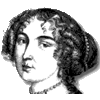
\includegraphics[scale=.25]{iamges/logo.png}}


%----------------------------------------------------------------------------------------------------------------------
% CUSTOM COMMANDS, ENVIRONMENTS AND COLORS

\newcommand{\pedbullet}[1]{\begin{itemize}\item #1 \end{itemize}}
\newcommand{\pedref}[1]{\hfill \cite{#1}}

\newenvironment{tip}[1]{\begin{block}{Tip}#1\end{block}}

\definecolor{lightblue}{cmyk}{.35, .10, 0, 0}

% customize the framezoom border color.
%\hypersetup{linkbordercolor={1 0 0}}

%----------------------------------------------------------------------------------------------------------------------
% DOCUMENT START, PREFIXES TITLE PAGE

\begin{document}
\frame{\titlepage}


%----------------------------------------------------------------------------------------------------------------------
% DOCUMENT OUTLINE

\section{Outline}
\subsection{Background}
\frame{
    \frametitle{Outline}
    \tableofcontents[hideallsubsections,part=1]
}
\subsection{Basic Analysis}
\frame{
    \frametitle{Outline}
    \tableofcontents[hideallsubsections,part=2]
}
\subsection{Advanced Analysis}
\frame{
    \frametitle{Outline}
    \tableofcontents[hideallsubsections,part=3]
}
\subsection{Custom Development}
\frame{
    \frametitle{Outline}
    \tableofcontents[hideallsubsections,part=4]
}


%----------------------------------------------------------------------------------------------------------------------
% INCLUDED SECTIONS

% included by ../header.tex

\part{Background Information}

\section{Introduction}
\subsection{Introduction}
\begin{frame}
    \frametitle{Instructors}
    \begin{block}{Pedram Amini}
        \begin{itemize}
            \item Manages the TippingPoint DVLabs Security Research Team
                \pedbullet{http://dvlabs.tippingpoint.com}
            \item Wrote PaiMei RE framework and Sulley fuzzing framework
            \item Founded OpenRCE.org
            \item Authored "Fuzzing: Brute Force Vulnerability Discovery"
        \end{itemize}
    \end{block}
    \begin{block}{Ero Carrera}
        \begin{itemize}
            \item Employed by Zynamics GmbH and Chief Research Officer at VirusTotal
            \item Reverse engineering, malware analysis and automation research
            \item Developer of \emph{pefile}, \emph{pydot}, \emph{pydasm}, \emph{ida2sql} and \emph{Pythonika}
        \end{itemize}
    \end{block}
\end{frame}

\begin{frame}
    \frametitle{What is Reverse Engineering?}
    \begin{definition}
        As it applies to software, reverse engineering is the process of unraveling the inner workings of a given system in the absence of source code.
    \end{definition}

    \begin{itemize}
        \item Also known as \alert{RE} or \alert{RCE}
        \item As simple as monitoring behavior from a high level
        \item As complex as reviewing individual instructions within an application
        \item Example questions reverse engineers seek to answer:
            \begin{itemize}
                \item What \alert{exactly} does this software do?
                \item Which lines of code are responsible for handling user input?
                \item How long can this parameter be before I corrupt the targets memory?
            \end{itemize}
    \end{itemize}
\end{frame}

\begin{frame}
    \frametitle{Who Hires Reverse Engineers?}
    \begin{itemize}
        \item Computer security firms, for discovering new software vulnerabilities
        \item AV companies, for analyzing new viruses and worms
        \item IPS vendors, for patch analysis
        \item Tuning shops, for dissecting ECUs
        \item Competitors, for unveiling your secret sauce
        \item Data recovery shops, for rebuilding specifications when source code is lost
    \end{itemize}
\end{frame}

\begin{frame}
    \frametitle{Questions for the Class}
    \begin{itemize}
        \item Who has past experience with IDA / disassembling?
        \item Who has past experience with OllyDbg / debugging?
        \item Who has past experience with Python?
        \item Who is a member of OpenRCE?
        \item Who has taken BH training before?
        \item Any professional reversers in the class?
    \end{itemize}
    \begin{block}{Introductions}
    Please introduce yourselves the first time you interact with one of us or the class. Name, country, company, favorite color, etc...
    \end{block}
\end{frame}

\begin{frame}
    \frametitle{Course Objectives}
    \begin{itemize}
        \item Learn the key concepts of Portable Executable files
        \item Create a functional and customized RCE environment
        \item Familiarize with industry standard tools and practices
        \item Gain real-world, hands on experience
        \item Wield the power of RCE to deal with common trickery
        \item Understand and subvert executable protections
        \item Apply cutting edge technologies to save analysis time
        \item Learn how to do all of the above quickly
            \pedbullet{You will be forced to put your mouse to rest ;-)}
        \item The class focus is on malware analysis, which is a vast field
            \pedbullet{We've selected subjects that we feel have real-world application}
    \end{itemize}
\end{frame}


\subsection{Malware Analysis}
\begin{frame}
    \frametitle{What is Malware Analysis?}
    \begin{definition}
        \emph{Malware Analysis} is the study of unknown code to discover it's purpose and functionality.
    \end{definition}
    \begin{itemize}
        \item Main goal
            \pedbullet{Glean relevant information in a timely manner}
            \pedbullet{Can not stress this point enough}
        \item Unfolding of a story
            \pedbullet{Each analysis technique may add another chapter to the story}
    \end{itemize}
\end{frame}

\begin{frame}
    \frametitle{Malware Classifications}
    \begin{itemize}
        \item Virus
            \pedbullet{Software which infects other applications and uses them as a spreading medium}
        \item Trojan
            \pedbullet{A malicious application which presents itself as something else}
        \item Worm
            \pedbullet{Code with the ability to spread from computer to computer by means of different network protocols}
        \item Spyware
            \pedbullet{Applications aiming to harvest personal information}
        \item Rootkit
            \pedbullet{Hidden tool/s providing stealth services to its writer}
    \end{itemize}
\end{frame}

\begin{frame}
    \frametitle{Malware Components}
    \begin{itemize}
        \item Infection
            \pedbullet{Exploit}
            \pedbullet{Social engineering}
        \item Payload
            \pedbullet{Destruction}
            \pedbullet{Theft}
            \pedbullet{Stealth}
            \pedbullet{Agent}
        \item Propagation
    \end{itemize}
\end{frame}

\begin{frame}
    \frametitle{A Look at Propagation}
    \begin{itemize}
        \item Low level attack vectors
            \pedbullet{Stack overflows}
            \pedbullet{Heap overflows}
            \pedbullet{Format string vulnerabilities}
        \item Higher level attack vectors
            \pedbullet{Browser exploitation}
        \item Highest level attack vectors
            \pedbullet{Social engineering}
            \pedbullet{Mass e-mails}
    \end{itemize}
\end{frame}


\subsection{Questions to Consider}
\begin{frame}
    \frametitle{How is it Spreading?}
    \begin{itemize}
        \item If over IP, how fast?
        \item Is the prand() biased?
        \item Does it contain a mass mailer?
        \item Does it spread over network shares?
        \item Does it spread over P2P or other file transfer mediums?
        \item Does it spread over an exploit?
    \end{itemize}
\end{frame}

\begin{frame}
    \frametitle{Does it Contain a Backdoor?}
    \begin{itemize}
        \item Does it connect to an IRC server?
        \item Does it bind to any ports?
        \item Does it retrieve data from the web?
        \item Does it retrieve data from news groups?
    \end{itemize}
\end{frame}

\begin{frame}
    \frametitle{What Modifications Are Made?}
    \begin{itemize}
        \item Does it create/modify/edit/delete any registry keys?
        \item Does it create/modify/edit/delete any files?
        \item Does it modify any running processes?
        \item Does it modify itself?
    \end{itemize}
\end{frame}

\begin{frame}
    \frametitle{Why Was it Written?}
    \begin{itemize}
        \item Depending on your goal this question could be the most important of all
        \item Targeted attack?
        \item Information theft?
        \item DDoS network?
    \end{itemize}
\end{frame}

\begin{frame}
    \frametitle{Who Wrote it?}
    \begin{itemize}
        \item What compiler was used?
        \item What date was it created on?
        \item What stylistic characteristics stand out?
    \end{itemize}
\end{frame}

\begin{frame}
    \frametitle{The Logical Three}
    \begin{itemize}
        \item We classify code into one of three logical categories:
        \item Constant code
            \begin{itemize}
                \item Code that is continuously running during execution
                \item Ex: IP Scanning loops, e-mail harvesting loops
            \end{itemize}
        \item Reactive code
            \begin{itemize}
                \item Code that is executed in reaction to an event
                \item Ex: An exploitable system was discovered
            \end{itemize}
        \item Dormant code
            \begin{itemize}
                \item Code that is designed to execute at a certain date
                \item Ex: coordinated DDoS attack
            \end{itemize}
    \end{itemize}
\end{frame}


\section{VM's and Live Analysis}
\subsection{Virtual Machines}
\begin{frame}
    \frametitle{Virtualization vs. Physical}
    \begin{itemize}
        \item Benefits of virtual machine (VM) technology
            \pedbullet{Fast and economical solution for lab environment deployment}
            \pedbullet{Network segregation can be virtualized}
            \pedbullet{Pre-infection system restore is painless}
        \item Pitfalls of virtual machine (VM) technology
            \pedbullet{Malware can detect the VM and alter behaviour}
            \pedbullet{Virtualization \emph{may} have bugs in replication of physical system}
        \item Should have at least one physical system in a malware lab
    \end{itemize}
    \begin{columns}
    \column{.7\textwidth}
        \begin{itemize}
            \item CoreRESTORE (www.coreprotect.com)
            \item Provides hardware level reboot-to-restore functionality
        \end{itemize}
    \column{.3\textwidth}
        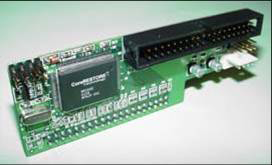
\includegraphics[scale=.40]{images/vms_and_live_analysis/corerestore.png} \\
    \end{columns}
\end{frame}

\begin{frame}
    \frametitle{x86 Virtual Machine Capabilities}
    \begin{itemize}
        \item x86 architecture does not meet Popek and Goldberg virtualization requirements
        \item Virtualization is accomplished via dynamic recompilation (like Java)
        \item This isn't all that important to know, just know that dynamic recompilation is slower than true self-virtualization
        \item AMD "Pacifica" and Intel "Vanderpool" have architecture level support for virtualization
    \end{itemize}
    \pedref{ACM-17-7}
\end{frame}

\begin{frame}
    \frametitle{Virtualization vs. Emulation}
    \begin{itemize}
        \item VM technologies such as VMware trap all hardware access and simulate the entire motherboard minus the processor
        \item Emulation technologies such as Bochs completely emulate the processor, hardware devices and memory
        \item Emulation is slower but provides greater flexibility of control and "safety" in terms of malware "breaking out" of the controlled environment
        \item Partial emulation can be very helpful in static analysis
    \end{itemize}
\end{frame}

\begin{frame}
    \frametitle{Virtual Machine Technologies}
    \begin{itemize}
        \item \alert{VMware}
            \pedbullet{VMWare server is now free}
        \item Microsoft Virtual PC (Connectix)
            \pedbullet{This is also free}
        \item Microsoft Virtual Server
        \item Plex86
        \item Xen
        \item Parallels
    \end{itemize}
\end{frame}

\begin{frame}
    \frametitle{Emulation Technologies}
    \begin{itemize}
        \item Bochs
            \pedbullet{The Bochs instrumentation library is badass, as Ero will show later}
        \item Qemu
        \item Chris Eagle's IDA x86-emu plug-in (partial emulation)
    \end{itemize}
\end{frame}


\begin{frame}
    \frametitle{VMWare Tips}
    \tip{Use a USB/Firewire disk for increased performance}
    \tip{Save snapshot disk space by installing new software from the network or CD}
\end{frame}


\subsection{Live Analysis}
\begin{frame}
    \frametitle{What and Why?}
    \begin{definition}
        Simply put, live analysis constitutes of running suspect code in a "sacrificial" environment while monitoring its activities at a high level
    \end{definition}

    \begin{itemize}
        \item Live analysis falls well short of reverse engineering
        \item However, it is still the most frequently used analysis technique
        \item A good starting point for "unfolding" the story
    \end{itemize}
\end{frame}

\begin{frame}
    \frametitle{SysInternals}
    \begin{itemize}
        \item SysInternals is home of Marc Russinovich
        \item Offers a number of excellent freeware and commercial utilities
        \item You know Marc from the Sony rootkit debacle
        \item More recently you may have heard of them due to the Best Buy Geek Squad scandal
        \item Most recently you may have heard of them because they sold to Microsoft
    \end{itemize}
\end{frame}

\begin{frame}
    \frametitle{SysInternals RegMon}
    \begin{itemize}
        \item Monitor all registry access in real time
        \item Supports filtering
    \end{itemize}
    \begin{center}
        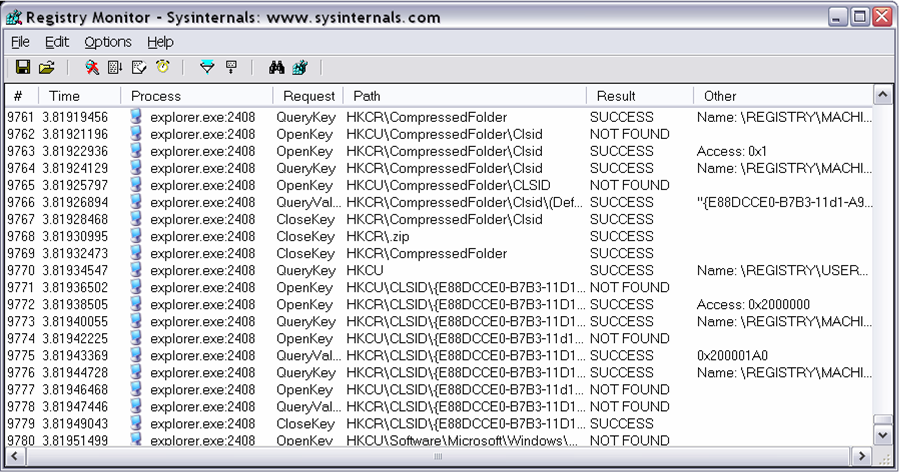
\includegraphics[scale=.35]{images/vms_and_live_analysis/regmon.png}
    \end{center}
\end{frame}

\begin{frame}
    \frametitle{SysInternals FileMon}
    \begin{itemize}
        \item Monitor all file access in real time
        \item Supports filtering
    \end{itemize}
    \begin{center}
        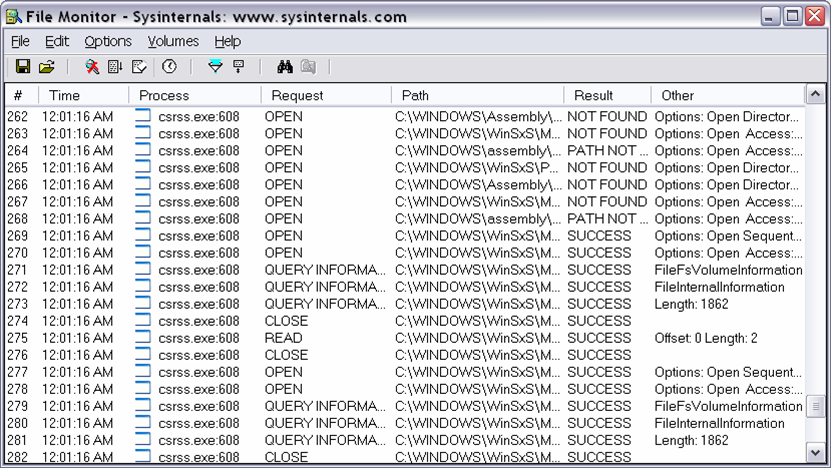
\includegraphics[scale=.35]{images/vms_and_live_analysis/filemon.png}
    \end{center}
\end{frame}

\begin{frame}
    \frametitle{SysInternals TCPView}
    \begin{itemize}
        \item Monitor all per-process socket endpoints in real time
            \pedbullet{ie: Determine what ports a specific process is bound to}
        \item Supports filtering
    \end{itemize}
    \begin{center}
        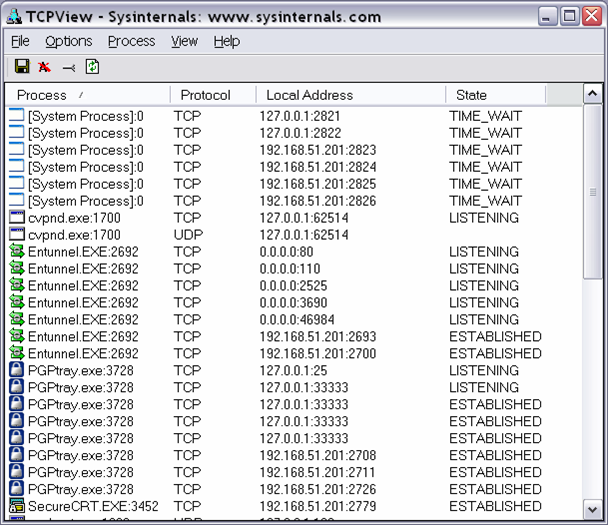
\includegraphics[scale=.30]{images/vms_and_live_analysis/tcpview.png}
    \end{center}
\end{frame}

\begin{frame}
    \frametitle{SysInternals Process Explorer}
    \begin{itemize}
        \item Task manager on steroids
        \item Exposes a plethora of useful information
    \end{itemize}
    \begin{center}
        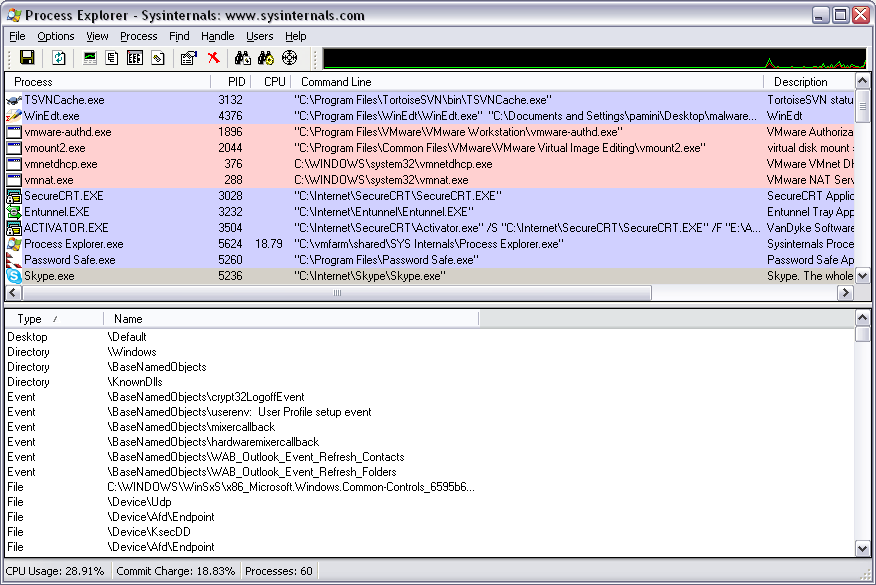
\includegraphics[scale=.30]{images/vms_and_live_analysis/process_explorer.png}
    \end{center}
\end{frame}

\begin{frame}
    \frametitle{InCtrl}
    \begin{columns}
    \column{.5\textwidth}
        \begin{itemize}
            \item Originally designed to monitor changes made by installers
            \item Applies well to malware
            \item Takes system "snapshots" pre/post execution
            \item Generates HTML report of monitors changes
        \end{itemize}
    \column{.5\textwidth}
        \begin{center}
            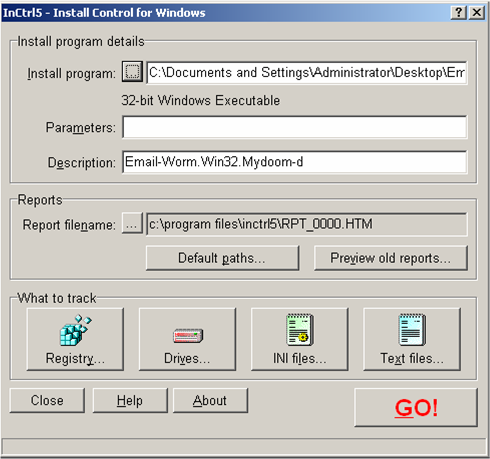
\includegraphics[scale=.5]{images/vms_and_live_analysis/inctrl.png} \\
        \end{center}
    \end{columns}
\end{frame}

\begin{frame}
    \frametitle{Wire Shark / Ethereal}
    \begin{columns}
    \column{.5\textwidth}
        \begin{itemize}
            \item Formerly known as Ethereal
            \item Wonderful and free network sniffer
            \item Can decipher a number of protocols
            \item Also vulnerable, very vulnerable
        \end{itemize}
    \column{.5\textwidth}
        \begin{center}
            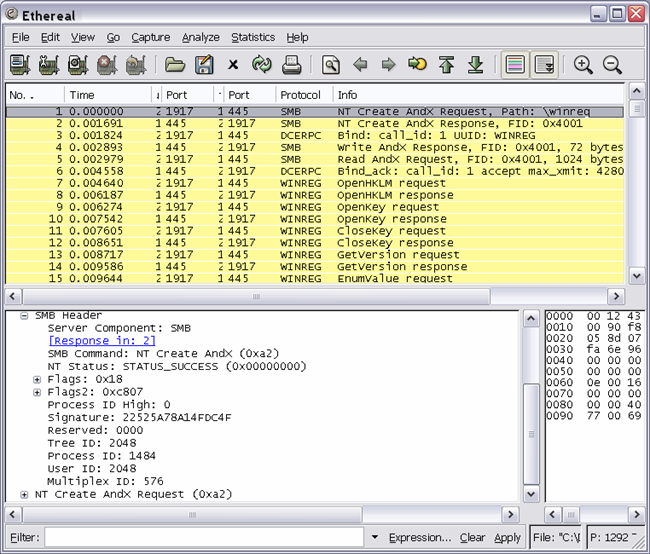
\includegraphics[scale=.30]{images/vms_and_live_analysis/ethereal.png} \\
        \end{center}
    \end{columns}
\end{frame}

\begin{frame}
    \frametitle{Dave Zimmer's Tools}
    \begin{itemize}
        \item Who is Dave Zimmer?
            \pedbullet{A VB coding machine}
            \pedbullet{His tools are currently available from http://labs.idefense.com}
        \item Malcode Analyst Pack
            \pedbullet{FakeDNS, IDCDumpFix, Mailpot, SCLog, ShellExt, Sniffhit, SocketTool}
        \item Multipot
            \pedbullet{Emulation based honeypot}
        \item SysAnalyzer
            \pedbullet{Like InCtrl, but specifically designed for malware}
    \end{itemize}
\end{frame}

\section{Architecture and OS}
\subsection{x86 Architecture}
\begin{frame}
    \frametitle{A 50,000ft View of the x86 Architecture}
    \begin{block}{}
        The main components of the x86 include the CPU, memory, disk and registers. The CPU operates on a fetch, decode and execute cycle.
    \end{block}
    \begin{itemize}
        \item Applications are implemented with individual \alert{assembly} instructions
        \item Individual instructions can:
            \pedbullet{Reference / manipulate memory}
            \pedbullet{Perform calculations}
            \pedbullet{Determine the \alert{next} instruction to execute}
        \item A \textit{single} line of high level code usually translates to \textit{multiple} instructions
        \item The x86 platform is considered \alert{CISC} vs RISC
    \end{itemize}
\end{frame}

\begin{frame}
    \frametitle{Introduction to Registers}
    \begin{itemize}
        \item There are 8 general purpose registers on 32-bit x86 platforms
        \item Each register is 32 bits long
        \item Register access is lowest latency (vs. memory or disk)
        \item As registers are valuable, compilers try to be intelligent with their usage
            \pedbullet{This factor comes into play during reversing}
    \end{itemize}
\end{frame}

\begin{frame}
    \frametitle{x86 General Purpose Registers}
    \begin{itemize}
        \item EAX
            \pedbullet{Volatile, accumulator, return value of functions}
        \item EBX
            \pedbullet{Non-volatile, base (indirect addressing)}
        \item ECX
            \pedbullet{Volatile, Counter, loop instructions}
        \item EDX
            \pedbullet{Volatile}
    \end{itemize}
    \begin{center}
        \begin{tabular}{|c|c|c|c|c|c|c|c|}                                     \hline
            8bits & 8bits & 8bits & 8bits & 8bits & 8bits & 8bits & 8bits   \\ \hline
            \multicolumn{8}{|c|}{\cellcolor{lightblue}RAX}                  \\ \hline
            & & & & \multicolumn{4}{|c|}{\cellcolor{red}EAX}                \\ \hline
            & & & & & & \multicolumn{2}{|c|}{\cellcolor{green}AX}           \\ \hline
            & & & & & & \cellcolor{orange}AH & \cellcolor{yellow}AL         \\ \hline
        \end{tabular}
    \end{center}
\end{frame}

\begin{frame}
    \frametitle{General Purpose Registers Continued}
    \begin{itemize}
        \item ESI
            \pedbullet{Non-volatile, string source}
        \item EDI
            \pedbullet{Non-volatile, string destination}
        \item ESP / EBP
            \pedbullet{Stack pointer (volatile) / frame pointer (non-volatile)}
        \item EIP
            \pedbullet{Instruction pointer}
    \end{itemize}
\end{frame}

\begin{frame}
    \frametitle{The Stack}
        \begin{definition}
            The stack is an abstract data structure supported by a combination of hardware and software features.
        \end{definition}
        \begin{itemize}
            \item Stack operations are \alert{L}ast \alert{I}n \alert{F}irst \alert{O}ut (\alert{LIFO})
            \item Think of it as a stack of dishes
            \item The \alert{\texttt{PUSH}} instruction places a 32-bit value on the stack
            \item The \alert{\texttt{POP}} instruction removes a 32-bit value from the stack
            \item The stack is used to pass parameters to functions
            \item The stack is used to maintain call chain state
            \item In Windows, the stack is used to store the \alert{S}tructured \alert{E}xception \alert{H}andling (\alert{SEH}) chain
        \end{itemize}
\end{frame}

\begin{frame}[fragile, label=debug]
    \frametitle{The Stack: Illustrated}
    \begin{columns}[T]
        \column{.5\textwidth}
            \begin{tiny}
            \begin{semiverbatim}
                0x43ce83b8: "pedram"
                0x43ce83bf: "amini"

                main:
                    \alert<2>{0x01 push 0xdeadbeef}
                    \alert<3>{0x02 pop eax}
                    \alert<4>{0x03 push 27}
                    \alert<5>{0x04 push 0x43ce83b8}
                    \alert<6>{0x05 push 0x43ce83bf}
                    \alert<7>{0x06 call copy_name}
                    \alert<17>{0x07 add esp, 0xc}
                    ...

                copy_name:
                    \alert<8>{0x20 push ebp}
                    \alert<9>{0x21 mov ebp, esp}
                    \alert<10>{0x22 sub esp, 0x100}
                    \alert<11>{0x23 lea eax, [ebp+0xc]}
                    \alert<12>{0x24 push eax}
                    \alert<13>{0x25 lea eax, [ebp-0x20]}
                    \alert<14>{0x26 push eax}
                    \alert<15>{0x27 call strcpy}
                    ...
                    \alert<16>{ret}
            \end{semiverbatim}
            \end{tiny}
        \column{.5\textwidth}
            \begin{tiny}
            \texttt{
            \begin{tabular}{r|c|l}
                              0x12FFFFFC & \cellcolor{gray}                                 0x00000000 & top of stack                       \\
                              0x12FFFF00 & \cellcolor{gray}                                 0x00000000 & end of SEH chain                   \\
                              0x12FFFF04 & \cellcolor{gray}                                 0x12345678 & SEH handler                        \\
                \only<2>     {0x12FFEFF8 & \cellcolor{yellow}                               0xDEADBEEF &                                    \\}
                \only<4-16>  {0x12FFEFF8 & \cellcolor{yellow}                               0x00000019 & 27                                 \\}
                \only<5-16>  {0x12FFEFF0 & \cellcolor{yellow}                               0x43CE83B8 & \emph{pedram}                      \\}
                \only<6-16>  {0x12FFEFEC & \cellcolor{yellow}                               0x43CE83BF & \emph{amini}                       \\}
                \only<7-15>  {0x12FFEFE8 & \cellcolor{red}                                  0x00000007 & return addr.                       \\}
                \only<8-15>  {0x12FFEFE4 & \cellcolor{orange}                               0x12FFEFF8 & saved frame                        \\}
                \only<10-15> {0x12FFEFE0 & \cellcolor{lightblue}\only<10-14>{ ....}\only<15-16>{ ..MA} & local vars                         \\}
                \only<10-15> {0x12FFEFC0 & \cellcolor{lightblue}\only<10-14>{ ....}\only<15-16>{ RDEP} & \only<14-15>{\alert{$\leftarrow$}} \\}
                \only<10-15> {0x12FFEEE0 & \cellcolor{lightblue}                                  .... &                                    \\}
                \only<12-15> {0x12FFEEDC & \cellcolor{yellow}                               0x43CE83B8 & \emph{pedram}                      \\}
                \only<14-15> {0x12FFEED8 & \cellcolor{yellow}                               0x12FFEFC0 & dst buff                           \\}
            \end{tabular}
            }
            \end{tiny}
    \end{columns}
\end{frame}


\subsection{Microsoft Windows OS}
\begin{frame}
    \frametitle{Microsoft Windows Memory Layout}
    \begin{columns}[T]
        \column{.5\textwidth}
            \begin{block}{Memory Space}
                \pause
                \uncover<+->{$2^{32}$}
                \uncover<+->{$= 4,294,967,296$ bytes} \\
                \uncover<+->{$ / 1024^3$}
                \uncover<+->{$= \alert<+->{4}$ \alert<.->{gigabytes}}
            \end{block}
        \column{.5\textwidth}
            \uncover<.->{\begin{block}{Memory Separation}
                The NT based platforms typically split the available 4 gigabytes of addressable memory into two halves; kernel and user.
            \end{block}}
    \end{columns}
    \uncover<+->{
        \begin{itemize}
            \item Each process "sees" it's own 2 gigabytes of virtual memory
                \pedbullet{This is possible thanks to \alert{memory paging}}
                \pedbullet{Processes can not "break out" of their memory space}
            \item The virtual address space is broken in \alert{pages}
                \pedbullet{Pages are typically \alert{4,096} bytes in size}
                \pedbullet{Memory permissions are applied at the page level}
        \end{itemize}
    }
\end{frame}

\begin{frame}
    \frametitle{Typical Memory Layout Diagram}
    \begin{columns}[T]
    \column{.5\textwidth}
        \begin{center}
        \begin{tiny}
        \texttt{
            \begin{tabular}{r|c|}
                             0x00000000 & \cellcolor{gray}USER SPACE                  \\
                             &                                                        \\
                \uncover<5->{0x00010000 & \cellcolor{yellow}Environment Variables     \\}
                             &                                                        \\
                \uncover<6->{0x00030000 & \cellcolor{orange}Heap                      \\}
                             &                                                        \\
                \uncover<7->{0x0012f000 & \cellcolor{red}Stack of Main Thread         \\}
                \uncover<6->{0x00150000 & \cellcolor{orange}Heap                      \\}
                             &                                                        \\
                \uncover<2->{0x00400000 & \cellcolor{green}Main Executable            \\}
                \uncover<2->{& \cellcolor{green}                                      \\}
                             &                                                        \\
                \uncover<8->{0x00d8d000 & \cellcolor{red}Stack of Thread 2            \\}
                             &                                                        \\
                \uncover<4->{0x71ab0000 & \cellcolor{green}WS2\_32.DLL                \\}
                             &                                                        \\
                \uncover<3->{0x7c800000 & \cellcolor{green}KERNEL32.DLL               \\}
                             &                                                        \\
                \uncover<3->{0x7c900000 & \cellcolor{green}NTDLL.DLL                  \\}
                             &                                                        \\
                \uncover<1->{0x7f000000 &
                \\}
                             0x80000000 & \cellcolor{gray}KERNEL SPACE                \\
            \end{tabular}
        }
        \end{tiny}
        \end{center}
    \column{.5\textwidth}
        \begin{block}{On Process Launch}
            \begin{itemize}
                \item<2-> Main image loaded into memory
                \item<3-> Required DLLs loaded into memory
                \item<5-> Environment variables mapped into memory
                \item<6-> Process heaps initialized
                \item<7-> Process stacks initialized
            \end{itemize}
        \end{block}
    \end{columns}
\end{frame}

\begin{frame}
  \frametitle{The Memory Layout Diagram}
  \begin{center}
    \pgfimage[height=7cm]{images/architecture_and_os/memory_layout}
  \end{center}
\end{frame}

\begin{frame}
    \frametitle{The Heap}
    \begin{itemize}
        \item Static allocations mostly originate from the stack
        \item The heap is the source of dynamic memory allocation
        \item There are multiple heap implementations
        \item Memory for the heap is allocated from user space
        \item The heap is essentially a number of doubly linked lists, organized by size
        \item Allocated blocks are removed from the free lists
        \item De-allocated blocks are placed back into the free lists
    \end{itemize}
\end{frame}

\begin{frame}
    \frametitle{SEH: Structured Exception Handling}
    \begin{itemize}
        \item Exception handlers are simply a registered function to refer to when "something bad happens"
        \item You can for example register an exception handler to handle attempts to divide by zero
        \item You can register more then one exception handler
        \item The \alert{chain} of exception handlers are stored on the stack
        \item When an exception occurs, the chain is walked to find an appropriate handler
        \item There is a catch-all handler, that's what generates the "Windows has detected a general protection fault" dialog
    \end{itemize}
\end{frame}

\begin{frame}
    \frametitle{Exercise}
    \begin{itemize}
        \item OllyDbg
            \pedbullet{Attach to or load calc.exe or notepad.exe}
            \pedbullet{Hit 'M' and verify memory layout}
        \item LordPE
            \pedbullet{Load calc.exe or notepad.exe}
            \pedbullet{Explore the various PE fields and directories}
            \pedbullet{We'll walk through the PE file format in depth in a minute}
    \end{itemize}
\end{frame}


\section{PE File Format}
\subsection{Overview and Headers}
\begin{frame}
    \frametitle{Portable Executable File Format}
    \begin{block}{History}
        Microsoft based the PE file format on the Unix COFF file format. As such it is sometimes referred to as PE/COFF.
    \end{block}
    \begin{itemize}
        \item \textit{Portable} in PE means
            \pedbullet{Supports both 32-bit and 64-bit}
            \pedbullet{Supports MIPS, DEC Alpha, PowerPC and ARM}
        \item Files with .exe extensions are PE
        \item Dynamic Link Libraries (DLLs) are PE
    \end{itemize}
\end{frame}

\begin{frame}
  \frametitle{PE Format Layout}
  \begin{center}
    \includegraphics<1>[height=7cm]{images/pe_format/PE_Format.pdf}%
  \end{center}
\end{frame}


\begin{frame}
  \frametitle{DOS and NT Headers Overview}
      \begin{itemize}
        \item These headers contain the very basic information to process \emph{PE} files
        \item A \emph{PE} file begins with the \emph{DOS} stub, usually responsible for the \emph{
�This program cannot be run in DOS mode�} message as well as location the \emph{PE} headers
        \item The PE headers contain the bulk of the information about the PE file
        \item Different sets of headers will be present depending on the type of data the PE file represents (an executable, a DLL, an object file)
      \end{itemize}
\end{frame}


\begin{frame}[t]
  \frametitle{DOS and NT Headers View}
  \begin{columns}[T]
    \begin{column}{6cm}
      \begin{itemize}
        \item PE files start with the DOS Header.
          \begin{itemize} \item e\_magic = \emph{4D5Ah} \alert{MZ} \end{itemize}
        \item NT headers comprise the FILE and the OPTIONAL headers.
          \begin{itemize} \item Signature = \emph{5045h} \alert{PE} \end{itemize}
      \end{itemize}
    \end{column}
    \begin{column}{7cm}
      \includegraphics<1>[width=6cm]{images/pe_format/PE-DOS_Header.pdf}%
    \end{column}
  \end{columns}
\end{frame}

\begin{frame}
  \frametitle{NT Headers: File Header View}
  \begin{center}
    \pgfimage[width=11cm]{images/pe_format/PE-FILE_Header}
  \end{center}
\end{frame}

\begin{frame}
  \frametitle{NT Headers: File Header}
  \begin{itemize}
    \item It's the first of the \emph{NT Headers} and \emph{File Header} follows immediately after the \emph{PE Signature}
    \item Contains some interesting fields
      \begin{itemize}
        \item \emph{Machine} indicates the target architecure for this file
        \item \emph{NumberOfSections}, the number of sections in the \emph{PE file}. This value is needed when exploring the section headers
        \item \emph{TimeDateStamp} is not of a critical importance, but some malware actually seems not to zero it so it might give some insight on the approximate release time... can be easily faked too
        \item \emph{SizeOfOptionalHeader} is an important element. Provides the exact size of the \emph{Optional Header} which is needed in order to properly parse the \emph{PE} file
      \end{itemize}
  \end{itemize}
\end{frame}




\begin{frame}
    \frametitle{NT Headers: Optional Header View}
    \begin{center}
        \pgfimage[height=7cm]{images/pe_format/PE-OPTIONAL_Header}
    \end{center}
\end{frame}


\begin{frame}
  \frametitle{NT Headers: Optional Header (1)}
  
  \begin{itemize}
    \item \emph{Magic} = \emph{10Bh} (PE32+ \emph{0x20b})
    \item \emph{AddressOfEntryPoint} is where execution of the executable code will begin (\alert{it's possible for other code within the executable to gain control before the entry point})
    \item \emph{ImageBase}. All relative address are based on this one. It's also usually possible to find the \emph{PE} header of the executable at this address in memory (unless it has been intentionally deleted)
    \item \emph{SectionAlignment} is the alignment of the sections in memory
    \item \emph{FileAlignment} is the alignment on disk
  \end{itemize}
\end{frame}


\begin{frame}
  \frametitle{NT Headers: Optional Header (2)}
  
  \begin{itemize}
    \item \emph{Operating system related fields} containing version specific information
    \item \emph{NumberOfRvaAndSizes} is the number of directory entries in the following array. Depending on how many there are the size of the \emph{Optional Header} will vary, something that some tools sometimes forget (assuming a constant default size)
    \item \emph{DataDirectory} is an array of structures pointing to additional information such as the \emph{Imports} and \emph{Exports} tables.
  \end{itemize}
\end{frame}



\begin{frame}
  \frametitle{Section Header View}
  \begin{center}
    \pgfimage[width=10cm]{images/pe_format/PE-SECTION_Header}
  \end{center}
\end{frame}

\begin{frame}
  \frametitle{Section Header}
  \begin{itemize}
        \item \emph{VirtualSize} is the size of the section once loaded in memory (can be bigger than \emph{SizeOfRawData}, in that case it's zero padded)
        \item \emph{VirtualAddress} is the address of the section in memory, relative to the \emph{ImageBase}
        \item \emph{SizeOfRawData} is the size of the section on disk (can be bigger than \emph{VirtualSize} due that its size is rounded at a \emph{FileAlignment} multiple)
        \item \emph{PointerToRawData} is the offset within the file to the contents to be loaded in memory (\emph{should} be a multiple of \emph{VirtualSize})
        \item \emph{Characteristics} contains flags with information such as whether the section can be executed, read, written into, etc.
  \end{itemize}
\end{frame}



\subsection{Interactive Walkthrough}
\begin{frame}
  \frametitle{DOS Header (1)}
  \begin{center}
    \pgfimage[height=8cm]{images/pe_file_inspection/slide_01}
  \end{center}
\end{frame}


\begin{frame}
  \frametitle{DOS Header (2)}
  \framezoom<1><2>[border=5](2.6cm,0cm)(7cm,3cm)
  \begin{center}
    \pgfimage[height=8cm]{images/pe_file_inspection/slide_01A}
  \end{center}
\end{frame}

\begin{frame}
  \frametitle{NT Headers (1)}
  \framezoom<1><2>[border=5](2.45cm,.5cm)(6.8cm,3cm)
  \begin{center}
    \pgfimage[height=8cm]{images/pe_file_inspection/slide_02}
  \end{center}
\end{frame}

\begin{frame}
  \frametitle{NT Headers (2)}
  \framezoom<1><2>[border=5](2.45cm,0.4cm)(7.3cm,3cm)
  \begin{center}
    \pgfimage[height=8cm]{images/pe_file_inspection/slide_03}
  \end{center}
\end{frame}

\begin{frame}
  \frametitle{NT Headers (3)}
  \framezoom<1><2>[border=5](2.28cm,.6cm)(8cm,3cm)
  \begin{center}
    \pgfimage[height=8cm]{images/pe_file_inspection/slide_03A}
  \end{center}
\end{frame}

\begin{frame}
  \frametitle{Optional Header (1)}
  \begin{center}
    \pgfimage[height=8cm]{images/pe_file_inspection/slide_04}
  \end{center}
\end{frame}

\begin{frame}
  \frametitle{Optional Header (2)}
  \framezoom<1><2>[border=5](1.3cm,2.67cm)(7cm,3cm)
  \begin{center}
    \pgfimage[height=8cm]{images/pe_file_inspection/slide_05}
  \end{center}
\end{frame}

\begin{frame}
  \frametitle{Directories (1)}
  \begin{center}
    \pgfimage[height=8cm]{images/pe_file_inspection/slide_06}
  \end{center}
\end{frame}

\begin{frame}
  \frametitle{Directories (2)}
  \framezoom<1><2>[border=5](1.33cm,2.5cm)(7.9cm,4.6cm)
  \framezoom<1><3>[border=5](1cm,2.88cm)(2.7cm,3.5cm)
  \framezoom<1><4>[border=5](4.1cm,2.7cm)(2.5cm,3.2cm)
  \begin{center}
    \pgfimage[height=7cm]{images/pe_file_inspection/slide_07}
  \end{center}%
\end{frame}

\begin{frame}
  \frametitle{Section Headers (1)}
  \begin{center}
    \pgfimage[height=7cm]{images/pe_file_inspection/slide_08}
  \end{center}
\end{frame}

\begin{frame}
  \frametitle{Section Headers (2)}
  \begin{center}
    \pgfimage[height=7cm]{images/pe_file_inspection/slide_09}
  \end{center}
\end{frame}

\begin{frame}
  \frametitle{Section Headers (3)}
  \framezoom<1><2>[border=5](2.67cm,3.76cm)(5.6cm,3.3cm)
  \begin{center}
    \pgfimage[height=7cm]{images/pe_file_inspection/slide_10}
  \end{center}
\end{frame}





\subsection{Import/Export Address Tables}

\begin{frame}
  \frametitle{Overview of the Import Address Table}
  \begin{itemize}
    \item The primary function of the \emph{Import Table} is to provide enough information to the loader to locate the API functions and other symbols needed by the executable
    \item It also provides us with a summary of the range of actions used by the executable
    \item Therefore hiding/obfuscating the \emph{Import Address Table} (\emph{IAT}) is a common technique in order to deprive analysts of a quick outlook
    \item The \emph{IAT} can be rebuilt by different packers/obfucators with varying degrees of complexity
  \end{itemize}
\end{frame}


\begin{frame}
  \frametitle{The Import Address Table Structures View}
  \begin{center}
    \includegraphics<1>[width=11cm]{images/pe_format/PE-Imports.pdf}
  \end{center}
\end{frame}


\begin{frame}
  \frametitle{The Import Address Table Structures Commented}
  \begin{block}{}
  The \emph{Import Address Table} information is distributed among three different structures. Repeated as necessary to describe the composing elements
  \end{block}
  \begin{itemize}
    \item The \emph{IMAGE\_IMPORT\_DESCRIPTOR} contains information about the \emph{DLL} containing the symbols to import
    \item The \emph{IMAGE\_THUNK\_DATA} contains information about the specific symbol imported
    \emph And finally, \emph{IMAGE\_IMPORT\_BY\_NAME} contains the name of the imported symbol if it's imported by name and not by ordinal alone
  \end{itemize}   
\end{frame}



\begin{frame}
  \frametitle{The IMAGE\_IMPORT\_DESCRIPTOR Structure}
  \begin{center}
    \includegraphics<1>[width=11cm]{images/pe_format/PE-Image_Import_Descriptor.pdf}
  \end{center}
\end{frame}


\begin{frame}
  \frametitle{The IMAGE\_IMPORT\_DESCRIPTOR Structure Commented}
  \begin{block}{}
    The \emph{IMAGE\_IMPORT\_DESCRIPTOR} contains information about the \emph{DLL} containing the symbols to import
  \end{block}
    \begin{itemize}
        \item \emph{OriginalFirstThunk} contains the relative address of the import table (a \emph{NULL} terminated array of \emph{IMAGE\_THUNK\_DATA} structures) containing the symbols to be imported
        \item \emph{Name} is the relative address of the name of the \emph{DLL} from which to import the symbols
        \item \emph{FirstThunk} is normally identical to \emph{OriginalFirstThunk} except after the imports have been resolved, when it will contain the addressses of the symbols
        \item If the imports are bound the \emph{TimeDateStamp} field will contain the timestamp of the referred DLL
    \end{itemize}
\end{frame}


\begin{frame}
  \frametitle{The IMAGE\_THUNK\_DATA Structure}
  \begin{center}
    \includegraphics<1>[width=11cm]{images/pe_format/PE-Image_Thunk_Data.pdf}
  \end{center}
\end{frame}

\begin{frame}
  \frametitle{The IMAGE\_THUNK\_DATA Structure Commented}  
  \begin{block}{}
    The \emph{IMAGE\_THUNK\_DATA} contains information about the specific symbol imported
  \end{block}
  \begin{itemize}
    \item \emph{ForwarderString} is not really used, \emph{Microsoft}'s docs no longer even mention this field
    \item \emph{Function} points to the data for the imported symbol when the image is bound or it has been resolved
    \item \emph{Ordinal} of the symbol to import
    \item \emph{AddressOfData} points to a \emph{IMAGE\_IMPORT\_BY\_NAME} structure with the name of the symbol to import
    \item The symbol is either imported by ordinal or name, this is indicated by the most significant bit, if set indicates the entry should be imported by ordinal and by name otherwise
  \end{itemize}
\end{frame}


\begin{frame}
  \frametitle{The IMAGE\_IMPORT\_BY\_NAME Structure Commented}
  \begin{block}{}
    \emph{IMAGE\_IMPORT\_BY\_NAME} contains the name of the symbol to import
  \end{block}
  \begin{itemize}
    \item \emph{Hint} is an index into the exported symbols table of the imported \emph{DLL}. Its purpose is to speed up load, if the symbol at that index matches the name then a sequential lookup can be skipped 
  \end{itemize} 
\end{frame}



\begin{frame}
  \frametitle{The Import Address Table}
  \begin{block}{}
  Executables wanting to hide imported symbols can resort to a large number of tricks. Usually they will resolve the imported symbols themselves and thus the \emph{IAT} will appear nearly empty. Some of the most popular ways of building the \emph{IAT} are
  \end{block}
  \begin{itemize}
    \item Manually going through the \emph{LoadLibrary}, \emph{GetProcAddress} sequence for all symbols
    \item Looking them up through hashes of their names
    \item Looking them up through signatures of their code
  \end{itemize}
  Once mapped, they can be integrated into the binary through
  \begin{itemize}
    \item Peculiar jump tables
    \item Skipping the \emph{DLL} function's entry point. It confuses import rebuilding techniques \emph{searching for} or \emph{hooking at} known \emph{DLL} function entry points
  \end{itemize}
\end{frame}


\begin{frame}
  \frametitle{The Export Table}
  \begin{block}{}
  Executable files such as applications and \emph{DLL}s can export symbols for other components to import
  \end{block}
  \begin{itemize}
    \item Both EXEs and DLLs can export symbols although EXEs rarely do so
    \item DLLs need to export symbols in order for other executables to import them
  \end{itemize}
\end{frame}

\begin{frame}
  \frametitle{The Export Table Structures}
  \begin{center}
    \includegraphics<1>[width=11cm]{images/pe_format/PE-Exports.pdf}%
  \end{center}
\end{frame}

\begin{frame}
  \frametitle{The IMAGE\_EXPORT\_DIRECTORY Structure Commented}
  \begin{block}{}
  The \emph{IMAGE\_EXPORT\_DIRECTORY} contains the information and pointers to code, the name and the ordinal for all exported symbols in the executable
  \end{block}
  \begin{itemize}
    \item \emph{Characteristics}, this field should always be 0 according to the specification
    \item \emph{TimeDateStamp}, \emph{MajorVersion} and \emph{MinorVersion} are self explanatory
    \item \emph{Name} points to a relative address containing the name of the \emph{DLL}
    \item \emph{NumberOfFunctions} is the number of pointers in the \emph{AddressOfFunctions} table
    \item \emph{NumberOfNames} is the number of entries in the \emph{AddresOfNames} table
  \end{itemize}
\end{frame}

\begin{frame}
  \frametitle{The IMAGE\_EXPORT\_DIRECTORY Structure Commented}
  \begin{block}{}
  \emph{AddressOfNames} and \emph{AddressOfNameOrdinals} run parallel, having an entry for each exported symbol, the name can be \emph{NULL}, the ordinal in \emph{AddressOfNameOrdinals} is used to find the symbol's data by indexing with it \emph{AddressOfFunctions}
  \end{block}
  \begin{itemize}
    \item \emph{AddressOfFunctions} points to an array of pointers containing the exported entries, it's indexed by an ordinal
    \item \emph{AddressOfNames} points to an array of pointers containing the names of the exported entries
    \item \emph{AddressOfNameOrdinals} points to an array of ordinals used to find the address of the exported data
  \end{itemize}
\end{frame}



\subsection{Updated PE32+ and Usage Examples}
\begin{frame}
  \frametitle{The Updated PE32+}
  \begin{itemize}
    \item The PE format has been expanded by Microsoft to accomodate for 64-bit architectures
    \item While on some other aspects the executables have changed, most of the PE headers remain largely untouched
    \item As a rule of thumb fields involving absolute addresses have been expanded to 8 bytes to accomodate for the 64-bit wide address space
    \item Fields containing RVAs remain as 4 bytes as the maximum image size is limited to 2GB and only 31-bits are necessary to address it all with relative addresses
  \end{itemize}
\end{frame}

\begin{frame}
  \frametitle{Updated Fields in the Optional Header}
  \begin{itemize}
    \item Optional header's \emph{Magic} number is in PE32+ \emph{0x20b}
    \item \emph{BaseOfData} has been removed from the Optional Header
    \item The following are now 64-bit wide \emph{ImageBase, SizeOfStackReserve, SizeOfStackCommit, SizeOfHeapReserve, SizeOfHeapCommit}
  \end{itemize}
\end{frame}

\begin{frame}
  \frametitle{Other Updated Fields}
  \begin{itemize}
    \item The following items have been updated in the IMAGE\_TLS\_DIRECTORY structure: \emph{StartAddressOfRawData, EndAddressOfRawData, AddressOfIndex, AddressOfCallBacks}
    \item And the following in the IMAGE\_LOAD\_CONFIG\_DIRECTORY: \emph{SecurityCookie, SEHandlerTable, SEHandlerCount}
  \end{itemize}
\end{frame}

\begin{frame}
  \frametitle{Curiosities of PE32+}
  \begin{itemize}
    \item Due to the new way of handling exceptions, the Exception Directory is supposed to contain most of the functions of the binary, more specifically, the "non-leaf" ones
    \item This enables tools to readily know most of the functions within a binary without having to rely on discovery through disassembly
  \end{itemize}
\end{frame}


\begin{frame}
    \frametitle{The Tiny PE challenge}
    Solareclipse took on the \emph{Tiny PE} challenge set by Gil Dabah about creating the smallest valid PE file. The result was:
    \begin{itemize}
        \item The smallest possible PE file: 97 bytes
        \item The smallest possible PE file on Windows 2000: 133 bytes
        \item The smallest possible PE file that downloads and executes a file over WebDAV: 133 bytes
    \end{itemize}
    \pedref{tinype}
\end{frame}


\begin{frame}
    \frametitle{The Tiny PE challenge}
    In order to achieve such small sizes the following steps were taken:
    \begin{itemize}
        \item Decreasing file alignment
        \item Removing the DOS stub
        \item Removing data directories
        \item Merging the section header within the Optional Header
        \item Merging the import table within the Optional Header
        \item Merging the IAT and DLL name
        \item Reusing the storage provided by non-used fields, only two matter in the DOS header
        \item Reducing the Optional Header size by truncating it at the minimum necessary length
    \end{itemize}
\end{frame}


\begin{frame}
  \frametitle{Additional Resources}
    \begin{block}<1->{Microsoft Portable Executable and Common Object File Format Specification}
        \pedref{MSPECOFF}
    \end{block}
    \begin{block}<1->{Portable Executable File Format � A Reverse Engineer View}
        \pedref{CBJ-PE}
    \end{block}
\end{frame}

% included by ../header.tex

\part{Basic Analysis}

\section{Overview of Analysis Tools}
\subsection{Debuggers}
\begin{frame}
    \frametitle{What is a Debugger?}
    \begin{definition}
        A debugger is a run-time analysis tool that allows you to instrument software at the assembly level.
    \end{definition}
    \begin{itemize}
        \item Common features include:
            \begin{itemize}
                \item CPU state information
                \item Single stepping
                \item Breakpoints
                \item Memory exploration and modification
                \item Thread enumeration
                \item PE file parsing
            \end{itemize}
    \end{itemize}
\end{frame}

\begin{frame}
    \frametitle{Unix Debuggers}
    \begin{itemize}
        \item GDB: The GNU Debugger
            \pedbullet{DDD: GUI front end}
        \item ADB
        \item Fenris, \alert{http://lcamtuf.coredump.cx/fenris}
        \item RR0D, \alert{http://rr0d.droids-corp.org}
            \pedbullet{This is actually an OS independent debugger, but there is no space on the next slide ;-)}
    \end{itemize}
\end{frame}

\begin{frame}
    \frametitle{Microsoft Windows Debuggers}
    \begin{itemize}
        \item Microsoft WinDbg
            \pedbullet{Powerful, freeware GUI debugging tool. Excellent for kernel development / abuse and security research}
        \item SoftICE
            \pedbullet{Powerful, expensive kernel debugger}
            \pedbullet{ICE = \alert{I}n \alert{C}ircuit \alert{E}mulator}
        \item OllyDbg
            \pedbullet{Powerful, freeware GUI debugging tool. Excellent for malware analysis and security research}
        \item IDA Pro
            \pedbullet{Clunky interface and difficult to use}
        \item PyDbg
            \pedbullet{Scripted debugger, sub-component of PaiMei}
    \end{itemize}
\end{frame}


\subsection{Disassemblers / Decompilers}
\begin{frame}
    \frametitle{What is a Disassembler?}
    \begin{definition}
        A disassembler is a static-analysis tool that translates raw bytes into assembly language, essentially the inverse of an assembler.
    \end{definition}
    \begin{itemize}
        \item There are many x86 disassembler libraries
        \item All debuggers have disassembling capabilities
        \item The hardest aspect of disassembly is differentiating between code vs. data
        \item There are less options for a solid pure disassembler ...
    \end{itemize}
\end{frame}

\begin{frame}
    \frametitle{DataRescue IDA Pro}
    \begin{itemize}
        \item The defacto standard in static analysis technology
        \item Supports multiple architectures
        \item Cross-platform, GUI and console
        \item Scriptable and pluggable
            \pedbullet{Lots of custom software written on this platform}
    \end{itemize}
\end{frame}

\begin{frame}[fragile]
    \frametitle{What is a Decompiler?}
    \begin{definition}
        A decompiler attempts to translate raw binary data into a higher level language than assembly. They generally fail miserably.
    \end{definition}
    \begin{itemize}
        \item \emph{"You can't get the toothpaste back in the tube"}
            \pedbullet{ie: \alert{True} decompilation is impossible}
        \item Some tools exist, for the most part they provide you with a more readable disassembly
    \end{itemize}
    \begin{uncoverenv}
        \begin{block}{}
            \begin{tiny}
            \begin{semiverbatim}
                if(*(ebp + 12) == -1)
                    eax = *( *(ebp + 8) * 4 + 0x422cc4);
                else
                    if((*(ebp + 12) & -8) != 0)
                        eax = eax | -1;
                    else
                        *(ebp - 4) = *(*(ebp + 8) * 4 + 0x422cc4);
                        ecx = *(ebp + 8);
            \end{semiverbatim}
            \end{tiny}
        \end{block}
    \end{uncoverenv}
\end{frame}

\begin{frame}
    \frametitle{Tools}
    \begin{itemize}
        \item REC
            \pedbullet{Useful (but unstable) command line tool}
            \pedbullet{We will give you a private IDA plug-in that can import REC output}
        \item REC Studio
            \pedbullet{GUI verson of REC}
            \pedbullet{Even more unstable}
        \item Desquirr
            \pedbullet{IDA plug-in}
            \pedbullet{Generates decent results but only does so in the messages window}
        \item Boomerang
            \pedbullet{Open source, worth keeping an eye on}
        \item Hex-Rays
            \pedbullet{Most recent of the tools}
            \pedbullet{IDA extension written by Ilfak of DataRescue}
    \end{itemize}
\end{frame}


\subsection{Other}
\begin{frame}
    \frametitle{Web Services}
    \begin{itemize}
        \item Virus Total (virustotal.com)
            \pedbullet{Online AV multi-scanner}
        \item Offensive Computing (offensivecomputing.net)
            \pedbullet{Malware zoo}
            \pedbullet{Over 600,000 samples}
        \item CWSandbox (cwsandbox.org)
            \pedbullet{COM, File, Mutex, Registry, Process information}
            \pedbullet{Network activity overview}
            \pedbullet{Human readable and machine parseable outputs (XML)}
        \item Anubis (anubis.iseclab.org)
            \pedbullet{Same as CW, adds PCAPs}
    \end{itemize}
\end{frame}


\subsection{Python}
\begin{frame}
    \frametitle{Syntax and Data Types}
    \begin{block}{}
        Whitespace matters. Use \emph{tabs} or \emph{spaces}, don't mix. No block delimiters.
    \end{block}
    \begin{itemize}
        \item This is an \textbf{int} (signed, 32bits) : 100
        \item This is a \textbf{long} (signed, infinite): 100L
        \item This is a \textbf{str}: "meow$\backslash$x00$\backslash$n" or 'meow$\backslash$x00$\backslash$n' (" $=$ ')
        \item This is a \textbf{tuple} (immutable): (10, 20, "25")
        \item This is a \textbf{list} (mutable): [10, 20, "25"]
        \item This is a \textbf{dict} (mutable): \{"one":1 , "two":2\}
        \item This is a \textbf{set} (mutable): set([1, 2, 3, 4])
    \end{itemize}
\end{frame}


\begin{frame}
    \frametitle{Keywords}
    \begin{block}{}
        29 keywords to rule them all
    \end{block}
    \begin{center}
    \begin{tabular}{|l|l|l|l|}
\hline
        \uncover{and & assert & break & class}
\\ \hline
        \uncover{continue & def & del & elif}
\\ \hline
        \uncover{else & except & exec & finally}
\\ \hline
        \uncover{for & from & global & if}
\\ \hline
        \uncover{import & in & is & lambda}
\\ \hline
        \uncover{not & or & pass & print}
\\ \hline
        \uncover{raise & return & try & while}
\\ \hline
        \uncover{yield & & &}
\\ \hline
    \end{tabular}
    \end{center}
\end{frame}


\begin{frame}[fragile, t]
    \frametitle{Conditionals, Loops and Exceptions}
    \begin{columns}[T]
        \column{.5\textwidth}
            \begin{block}{}
                \begin{tiny}
                \begin{semiverbatim}
if \emph{conditional}:
    \emph{instruction}
    \emph{instruction}
elif \emph{conditional}:
    \emph{instruction}
else:
    \emph{instruction}
    \emph{instruction}
                \end{semiverbatim}
                \end{tiny}
            \end{block}
        \column{.5\textwidth}
            \begin{block}{}
                \begin{tiny}
                \begin{semiverbatim}
for \emph{x} in \emph{set}:
    \emph{instruction}

for \emph{x} in xrange(\emph{100}):
    \emph{instruction}

while \emph{conditional}:
    \emph{instruction}
                \end{semiverbatim}
                \end{tiny}
            \end{block}
    \end{columns}
    \begin{block}{}
        \begin{tiny}
        \begin{semiverbatim}
try:
    \emph{instruction}
except:
    \emph{instruction}
else:
    \emph{instruction}
        \end{semiverbatim}
        \end{tiny}
    \end{block}
    \begin{itemize}
        \item Python essentially reads like pseudo code
        \item Pencil + napkin + 10 minutes $=$ Python code
    \end{itemize}
\end{frame}

\begin{frame}[fragile, t]
    \frametitle{Functions and Classes}
    \begin{columns}[T]
        \column{.5\textwidth}
            \begin{block}{Functions}
                \begin{tiny}
                \begin{semiverbatim}
def do\_something (\emph{arg}):
    \emph{instruction}
    return \emph{something}

def do\_something (\emph{arg1}, \emph{arg2}=10, \emph{arg3}=20):
    \emph{instruction}

do\_something(1, 5)
do\_something(1, arg3=50)
                \end{semiverbatim}
                \end{tiny}
            \end{block}
        \column{.5\textwidth}
            \begin{block}{Classes}
                \begin{tiny}
                \begin{semiverbatim}
class my\_class:
    def \_\_init\_\_ (self, \emph{arg}):
        \emph{instruction}

    def member\_routine(self, \emph{arg}):
        \emph{instruction}
        return \emph{something}

class inherit (my\_class):
                \end{semiverbatim}
                \end{tiny}
            \end{block}
    \end{columns}
    \begin{itemize}
        \item Functions can take a variable number of arguments
        \item You can specify some or all of the optional arguments
        \item Use classes to define structures
    \end{itemize}
\end{frame}


\section{(Dis)Assembly}
\subsection{Crash Course}
\begin{frame}
    \frametitle{The Very Basics}
    \begin{itemize}
        \item We look at \alert{Intel} (vs. AT\&T) style assembler
            \pedbullet{ex: MOV destination, source}
        \item Brackets are like a pointer dereference
            \pedbullet{ex: *EAX = [EAX] = dword ptr [EAX]}
        \item LEA is \alert{L}oad \alert{E}ffective \alert{A}ddress
        \begin{itemize}
            \item Transfers offset address of source to destination register
            \item It's actually faster to use the MOV instruction
                \pedbullet{ex: LEA EAX, [EBX] vs. MOV EAX, EBX}
            \item You'll see LEA frequently used for basic math operations
                \pedbullet{ex: LEA EAX, [EAX*EAX] is equivalent to $EAX^2$}
        \end{itemize}
    \end{itemize}
\end{frame}

\begin{frame}
    \frametitle{The Very Basics Continued}
    \begin{itemize}
        \item XOR-ing a register with itself zeroes it
            \pedbullet{ex: XOR EAX, EAX $\rightarrow$ EAX = 0}
        \item Numbers, signed vs. unsigned
        \begin{itemize}
            \item Unsigned positives range from \alert{0} through \alert{0xFFFFFFFF}
            \item Signed representation splits the range in half
                \pedbullet{Positives range from \alert{0x00000000} through \alert{0x7FFFFFFF}}
                \pedbullet{Negatives range from \alert{0x80000000} through \alert{0xFFFFFFFF} (-1)}
        \end{itemize}
    \end{itemize}
\end{frame}

\begin{frame}
    \frametitle{Even More Basics}
    \begin{itemize}
        \item PUSHA(D) / POPA(D)
            \pedbullet{Save / restore all registers}
        \item PUSHF(D) / POPF(D)
            \pedbullet{Save / restore all CPU flags}
        \item The 'D' instructions are 32bit, otherwise 16bit
    \end{itemize}
\end{frame}

\begin{frame}
    \frametitle{Memory Addressing Modes}
    \begin{itemize}
        \item Immediate addressing mode
            \pedbullet{\texttt{int big\_num = 0xDEADBEEF;}}
            \pedbullet{\texttt{MOV EAX, \alert{0xDEADBEEF}}}
        \item Direct addressing mode
            \pedbullet{\texttt{int big\_num = 0xDEADBEEF; b;}}
            \pedbullet{\texttt{b = *( \&big\_num );}}
            \pedbullet{\texttt{MOV EAX, \alert{[0x40508c]}}}
        \item Indirect addressing mode
            \pedbullet{\texttt{char first\_initial = *name;}}
            \pedbullet{\texttt{MOV AL, \alert{[EBX]}}}
        \item Indexed addressing mode
            \pedbullet{\texttt{int chosen = char\_array[0xC01a];}}
            \pedbullet{\texttt{MOV EAX, \alert{[EBX+0xC01A]}}}
        \item Scaled indexed addressing mode
            \pedbullet{\texttt{some\_struct *mystruct = struct\_array[20];}}
            \pedbullet{\texttt{MOV EAX, \alert{[EBX+ECX*20]}}}
    \end{itemize}
\end{frame}

\begin{frame}
    \frametitle{Instructions You Need to Know About}
    \begin{itemize}
        \item INC, DEC, ADD, SUB, MUL, DIV
            \pedbullet{Basic math instructions}
        \item MOV, LEA
            \pedbullet{Manipulate memory and registers}
        \item CALL / RET, ENTER / LEAVE
            \pedbullet{Transfer control to / back from another function}
        \item CMP, TEST
            \pedbullet{Compare values}
        \item JMP, JZ, JNZ, JG, JL, JGE, etc...
            \pedbullet{Transfer control flow to another instruction}
        \item PUSH, POP
            \pedbullet{Put items on / take items off of the stack}
        \item AND, OR, XOR, SHL, SHR
            \pedbullet{Bitwise operations}
    \end{itemize}
\end{frame}

\begin{frame}
    \frametitle{CPU Flags You Need to Know About}
    \begin{itemize}
        \item CPU flags stored in a 32-bit EFLAGS register
        \item \alert{ZF}, Zero Flag
            \pedbullet{Updated when the result of an operation is zero}
            \pedbullet{Used for JZ, JNZ etc..}
        \item \alert{SF}, Sign Flag
            \pedbullet{1 denotes negative number}
            \pedbullet{0 denotes positive number}
        \item \alert{OF}, Overflow Flag
            \pedbullet{Used in combination with ZF/SF for JG, JGE etc ...}
        \item \alert{CF}, Carry Flag (also an overflow indicator)
            \pedbullet{Used in combination with ZF for JA, JAE etc ...}
    \end{itemize}
\end{frame}


\subsection{Assembly Patterns}
\begin{frame}
    \frametitle{Calling Conventions}
    \begin{itemize}
        \item cdecl
            \pedbullet{Caller cleans up the stack}
        \item stdcall
            \pedbullet{Callee cleans up the stack}
        \item fastcall
            \pedbullet{Arguments can be passed in registers}
            \pedbullet{Microsoft: ECX and EDX (stdcall stack handling)}
            \pedbullet{Borland: EAX, ECX and EDX (also stdcall)}
        \item thiscall
            \pedbullet{C++ code, object pointer is passed in a register}
            \pedbullet{Microsoft: ECX}
            \pedbullet{Borland / Watcom: EAX}
        \item naked
    \end{itemize}
\end{frame}

\begin{frame}[fragile]
    \frametitle{Function Calls}
    \begin{columns}[T]
        \column{.5\textwidth}
            \begin{block}{stdcall}
                \begin{tiny}
                \begin{semiverbatim}
                    \alert{some_function(arg1, arg2);}

                    push arg2
                    push arg1
                    call some_function
                    mov [ebp-0xc], eax

                \end{semiverbatim}
                \end{tiny}
            \end{block}
        \column{.5\textwidth}
            \begin{block}{cdecl}
                \begin{tiny}
                \begin{semiverbatim}
                    \alert{some_function(arg1, arg2);}

                    push arg2
                    push arg1
                    call some_function
                    add esp, 8
                    mov [ebp-0xc], eax
                \end{semiverbatim}
                \end{tiny}
            \end{block}
    \end{columns}
    \begin{itemize}
        \item Function arguments are pushed in inverse order
        \item The above-left snippet demonstrates \alert{stdcall} calling convention.
            \pedbullet{The \emph{callee} cleans up the stack}
            \pedbullet{Recall that with \alert{cdecl} the \emph{caller} cleans up the stack}
        \item Can anyone guess why there is a need for stdcall vs cdecl?
    \end{itemize}
\end{frame}

\begin{frame}[fragile]
    \frametitle{EBP-Based Framing}
    \begin{columns}[T]
        \column{.5\textwidth}
            \begin{block}{Traditional}
            \begin{tiny}
            \begin{semiverbatim}
                push ebp
                mov ebp, esp
                sub esp, 0x100
            \end{semiverbatim}
            \end{tiny}
            \end{block}
        \column{.5\textwidth}
            \begin{block}{Recent OS DLLs}
            \begin{tiny}
            \begin{semiverbatim}
                mov edi, edi
                push ebp
                mov ebp, esp
            \end{semiverbatim}
            \end{tiny}
            \end{block}
    \end{columns}
    \begin{itemize}
        \item Optimized compiles may omit the frame pointer
            \pedbullet{In which case, local variables are referenced from ESP}
        \item \texttt{mov edi, edi}
            \pedbullet{Effectively a 2-byte NOP}
            \pedbullet{Why didn't they just use NOP, NOP?}
    \end{itemize}
\end{frame}

\begin{frame}
    \frametitle{Return Values}
    \begin{itemize}
        \item Saving the return value from a call
    \end{itemize}
    \begin{center}
        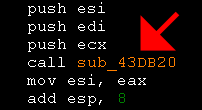
\includegraphics[scale=.75]{images/disassembly/return_value.png} \\
    \end{center}
\end{frame}

\begin{frame}[label=current]
    \frametitle{'\alert{P}' - \alert{P}arameters are \alert{P}ositive}
    \begin{itemize}
        \item \alert{P}arameters passed to a function are referenced \alert{P}ositive from EBP
            \pedbullet{\texttt{[EBP $+$ values]} are typically arguments on the stack}
            \pedbullet{\texttt{[EBP - values]} are typically local variables}
    \end{itemize}
\end{frame}

\begin{frame}[fragile]
    \frametitle{Branching}
    \begin{center}
        When reading a CMP statement, remember that the left side operand is the one being compared against.  The trick is to think \alert{"is..."}:
    \end{center}
    \begin{block}{}
        \begin{tiny}
        \begin{semiverbatim}
            ebx       = 0
            [eax+14h] = 1

            cmp     ebx, [eax+14h]  // think: \alert{is ebx...}
            ja      T1              // above? , 0 > 1 no jump
            jb      T2              // below? , 0 < 1 jumps
            je      T1              // equal? , 0 = 0 no jump
            cmp    [eax+14h], ebx   // think: \alert{is [eax+14h]...}
            ja      T2              // above? , 1 > 0 jumps
            jb      T1              // below? , 1 < 0 no jump
            je      T2              // equal? , 1 = 0 no jump
        \end{semiverbatim}
        \end{tiny}
    \end{block}
\end{frame}

\begin{frame}[fragile]
    \frametitle{Conditional Blocks}
    \begin{block}{}
        \begin{tiny}
        \begin{semiverbatim}
            \alert{if (length > 128)}
                \alert{length = 128;}

                mov eax, [ebp+8]
                cmp eax, 0x80
                jbe skip
                mov eax, 0x80
            skip:
                ...
        \end{semiverbatim}
        \end{tiny}
    \end{block}
    \begin{itemize}
        \item JBE (\alert{J}ump \alert{B}elow or \alert{E}qual) is an unsigned comparison
        \item vs. JLE (\alert{J}ump if \alert{L}ess than or \alert{E}qual) is a signed comparison
        \item While we're on the subject of signedness
            \pedbullet{MOVSX vs. MOVZX}
    \end{itemize}
\end{frame}

\begin{frame}[fragile]
    \frametitle{Loops}
    \begin{block}{}
        \begin{tiny}
        \begin{semiverbatim}
            \alert{for (i = 0; i < 100; i++)}
                \alert{do_something();}

                xor ecx, ecx
            start:
                cmp ecx, 0x64
                jge exit
                call do_something
                inc ecx
                jmp start
            exit:
        \end{semiverbatim}
        \end{tiny}
    \end{block}
    \begin{itemize}
        \item Loops are easier to spot in graphs
            \pedbullet{We'll talk more about this later}
            \pedbullet{IDA Plug-ins exist for automating loop detection}
    \end{itemize}
\end{frame}

\begin{frame}[fragile]
    \frametitle{Switch Statements}
    \begin{block}{}
        \begin{tiny}
        \begin{semiverbatim}
            \alert{switch (var) \{}
                \alert{case 0: var = 100; break;}
                \alert{case 1: var = 200; break;}
                \alert{...}

                jmp switch_table[eax*4]
            case_0:
                mov [ebp-4], 100
                jmp end
            case_1:
                mov [ebp-4], 200
                jmp end
                ...
            end:
        \end{semiverbatim}
        \end{tiny}
    \end{block}
    \begin{itemize}
        \item Both IDA and OllyDbg have excellent switch/case detection
    \end{itemize}
\end{frame}

\begin{frame}[fragile]
    \frametitle{Inline memcpy() / strcpy()}
    \begin{block}{}
        \begin{tiny}
        \begin{semiverbatim}
            mov esi, source
            mov edi, [ebp-64]
            mov ebx, ecx
            shr ecx, 2
            \alert{rep movsd}
            mov ecx, ebx
            and ecx, 3
            \alert{rep movsb}
        \end{semiverbatim}
        \end{tiny}
    \end{block}
    \begin{itemize}
        \item The \alert{rep movsd} copies ECX dwords from ESI to EDI
        \item The \alert{rep movsb} copies the remainder of the bytes
    \end{itemize}
\end{frame}

\begin{frame}[fragile]
    \frametitle{Inline strlen()}
    \begin{block}{}
        \begin{tiny}
        \begin{semiverbatim}
            mov edi, string
            or ecx, 0xFFFFFFFF
            xor eax, eax
            \alert{repne scasb}
            \alert{not ecx}
            \alert{dec ecx}
        \end{semiverbatim}
        \end{tiny}
    \end{block}
    \begin{itemize}
        \item The \alert{repne scasb} The repne scasb instruction scans the string in EDI for the character stored in AL (NULL in this case)
        \item For each scanned character ECX is decremented and EDI is incremented
        \item At the end of the REPNE sequence
            \begin{itemize}
                \item EDI = found char + 1
                \item ECX = negative string length minus two
                    \pedbullet{Logical not, minus one = string length}
            \end{itemize}
    \end{itemize}
\end{frame}

\begin{frame}[fragile]
    \frametitle{Structure Access}
    \begin{block}{}
        \begin{tiny}
        \begin{semiverbatim}
            push ebp
            mov ebp, esp
            mov \alert{eax}, off_deadbeef
            push ebx
            mov ebx, [ebp+arg_0]
            push esi
            cmp ebx, [\alert{eax}+14h]
            push edi
            ja short loc_12345678
            cmp [\alert{eax}+8], ebx
            sbb esi, esi
        \end{semiverbatim}
        \end{tiny}
    \end{block}
    \begin{itemize}
        \item EAX is loaded from a global variable
        \item Also, [] is used with EAX, which means this global variable is a pointer
    \end{itemize}
\end{frame}

\begin{frame}[fragile]
    \frametitle{Division}
    \begin{itemize}
        \item The 'div' instruction is \textbf{incredibly} slow. Compilers don't use it, unless they need the remainder
        \item Instead, divides are typically seen as a combination of shift instructions
        \item The following instruction divides EAX by 4:
            \pedbullet{\texttt{SHR EAX, 2}}
    \end{itemize}
\end{frame}

\begin{frame}[fragile]
    \frametitle{Pseudo Random Numbers}
    \begin{block}{Slammer MSSQL Worm PRND Engine}
        \begin{tiny}
        \begin{semiverbatim}
            MOV    0XFFFFFFB4(%EBP),%EAX ; eax = GetTickCount()
            LEA    (%EAX,%EAX,2),%ECX    ; ecx = eax + eax * 2
            LEA    (%EAX,%ECX,4),%EDX    ; edx = eax + ecx * 4
            SHL    $0X4,%EDX             ; edx = edx << 4 (edx *= 2^4 (16))
            ADD    %EAX,%EDX             ; edx += eax
            SHL    $0X8,%EDX             ; edx = edx << 8 (edx *= 2^8 (256))
            SUB    %EAX,%EDX             ; edx -= eax
            LEA    (%EAX,%EDX,4),%EAX    ; eax = eax + edx * 4
            ADD    %EBX,%EAX             ; eax += ebx
            MOV    %EAX,0XFFFFFFB4(%EBP) ; store target address
        \end{semiverbatim}
        \end{tiny}
    \end{block}
    \begin{itemize}
        \item Sorry, this is a different flavor of assembly (old excerpt)
        \item "Random" numbers are frequently generated via large multiplications that rely on integer wrapping
        \item The above excerpt is equivalent to multiplying by 214,013
    \end{itemize}
\end{frame}

\begin{frame}
    \frametitle{Type Recovery}
    \begin{itemize}
        \item There is no type representation at the assembly level
        \item We need to differentiate...
            \pedbullet{Strings from raw data}
            \pedbullet{UNICODE strings from ASCII strings}
            \pedbullet{Integers from pointers}
            \pedbullet{Integers from booleans}
        \item Sometimes type recovery requires examination across function boundaries
        \item Type recovery is simple for documented API calls
    \end{itemize}
\end{frame}

\begin{frame}
    \frametitle{Type Recovery: Integers vs. Pointers}
    \begin{itemize}
        \item Integers are \alert{never} dereferenced
        \item Integers are frequently compared, pointers are not
        \item Pointers are compared against zero or other pointers
        \item Arithmetic on pointers is simple, potentially complex for integers
    \end{itemize}
\end{frame}

\begin{frame}
    \frametitle{Type Recovery: Strings vs. Raw Data}
    \begin{itemize}
        \item String copying is generally prefixed with a strlen() (or inline equivalent)
            \pedbullet{Raw data copies will not have a prefixed strlen()}
        \item Strings are often compared against readable characters and other strings
            \pedbullet{Raw data may not be}
        \item Trace string parameters down to API calls!
    \end{itemize}
\end{frame}

\begin{frame}[fragile]
    \frametitle{C++ (Object Oriented) Code}
    \begin{itemize}
        \item As mentioned before, the \alert{this} pointer is typically passed to function through ECX
    \end{itemize}
    \begin{block}{}
        \begin{tiny}
        \begin{semiverbatim}
            lea ecx, [esp+16]
            call member_routine
        \end{semiverbatim}
        \end{tiny}
    \end{block}{}
    \begin{itemize}
        \item Virtual Tables or VTables, are commonly seen in C++. Example:
    \end{itemize}
    \begin{block}{}
        \begin{tiny}
        \begin{semiverbatim}
            mov eax, esi
            push 0x100
            call dword ptr [eax+50]
        \end{semiverbatim}
        \end{tiny}
    \end{block}{}
    \begin{itemize}
        \item When reversing arbitrary objects or structures locating initialization routines such as constructors / destructors can prove helpful
    \end{itemize}
\end{frame}

\begin{frame}
    \frametitle{Branchless Logic}
    \begin{itemize}
        \item Compilers will avoid branching if possible
        \item Many simple compare / branch pairs can be converted into a sequence of arithmetical operations
        \item The usage of the \alert{\texttt{sbb}} instruction is a typical indicator
        \item The resulting code runs faster, but is not as readable for human analysis
    \end{itemize}
\end{frame}

\begin{frame}[fragile]
    \frametitle{Branchless Logic: Example}
        \begin{block}{}
            \begin{semiverbatim}
                cmp     eax, 1
                sbb     eax, eax
                inc     eax
                pop     esi
                pop     ebx
                retn
            \end{semiverbatim}
        \end{block}
        \begin{itemize}
            \item<+-> \alert{cmp eax, 1} will set the carry flag (\alert{CF}) if \alert{eax} is 0
            \item<+-> \alert{sbb eax, eax} does \alert{eax = eax - (eax+CF)}
            \item<+-> Therefore if \alert{eax} was 0 we have \alert{eax = 0 - (0+1) = -1}
            \item<+-> Otherwise if \alert{eax} is greater than 0 we have \alert{eax = eax - eax+0 = 0}
            \item<+-> The increment will set the possible \alert{eax} values to 1 or 0
        \end{itemize}
\end{frame}

\begin{frame}[fragile]
    \frametitle{Mastering These Concepts}
    \begin{itemize}
        \item Reverse engineering isn't as much a matter of difficulty as it is a matter of familiarization and practice
        \item The best way to learn is hands on experience
            \begin{itemize}
                \item Keep a quick reference handy (see opcodes.hlp)
                \item Single step with a debugger
                \item Use an emulator
                \item Disassemble familiar code
                    \pedbullet{Compile and disassemble small snippets of code}
            \end{itemize}
    \end{itemize}
\end{frame}


\section{IDA Pro}
\subsection{Overview}
\begin{frame}
    \frametitle{Introduction to IDA Pro}
    \begin{itemize}
        \item IDA is \alert{the} tool for reverse engineering
        \item IDA is commercial, costs roughly \$450 US
        \item Scriptable through IDC / IDAPython
        \item Pluggable through a multitude of languages
        \item \alert{Interactive} Disassembler Pro
            \begin{itemize}
                \item It's named interactive for a reason. IDA makes mistakes and won't recognize everything correctly
                \item However, you can interact with the database and correct the errors
            \end{itemize}
        \item FLIRT
            \begin{itemize}
                \item \alert{F}ast \alert{L}ibrary \alert{I}dentification and \alert{R}ecognition \alert{T}echnology
                \item Allows IDA to recognize standard library calls
            \end{itemize}
    \end{itemize}
\end{frame}

\begin{frame}
    \frametitle{Executable Files}
    \mode<article>
    {
        \begin{itemize}
            \item idag.exe: Microsoft Windows GUI
            \item idaw.exe: Microsoft Windows text interface
            \item idau.exe: Microsoft Windows / MSDOS generic text interface
            \item win32\_remote.exe: Remote Windows debugger client
            \item linux\_server / linux\_server64: Remote Linux debugger client
        \end{itemize}
    }
    \mode<presentation>
    {
        idag.exe \dotfill Microsoft Windows GUI                                 \\
        idaw.exe \dotfill Microsoft Windows text interface                      \\
        idau.exe \dotfill Microsoft Windows / MSDOS generic text interface      \\
        win32\_remote.exe \dotfill Remote Windows debugger client               \\
        linux\_server / linux\_server64 \dotfill Remote Linux debugger client
    }
\end{frame}

\begin{frame}
    \frametitle{File Types}
    \mode<article>
    {
        \begin{itemize}
            \item .CFG: Configuration file
            \item .IDC: IDA Script
            \item .IDB: IDA Database
        \end{itemize}
    }
    \mode<presentation>
    {
        .CFG \dotfill Configuration file \\
        .IDC \dotfill IDA Script         \\
        .IDB \dotfill IDA Database       \\
    }
    \begin{itemize}
        \item Processor modules
            \pedbullet{Windows: .W64, .W32, .D32, .DLL}
            \pedbullet{Linux: .IL64, .ILX}
        \item Loader modules
            \pedbullet{Windows: .L64, .LDW, .LDX, .LDO}
            \pedbullet{Linux: .LLX64, .LLX}
        \item Plug-in modules
            \pedbullet{Windows: .P64, .PLW, .PLD, .PL2}
            \pedbullet{Linux: .PLX64, .PLX}
    \end{itemize}
\end{frame}

\begin{frame}
    \frametitle{IDA Autoanalysis Algorithm}
    \begin{block}{}
        The autoanalysis algorithm is not documented, but it can be roughly described as follows (this was verified by Ilfak):
    \end{block}
    \begin{enumerate}
        \item Load the file in the database and create segments
        \item Add the entry point and all DLL exports to the analysis queue
        \item Find all typical code sequences and mark them as code. Add their addresses to the analysis queue
        \item Get an address from the queue and disassemble the code at that address, adding all code references to the queue
        \item While the queue is not empty, go to 4
        \item Make a final analysis pass, converting all unexplored bytes in the text section to code or data
    \end{enumerate}
    \pedref{csw06-sotirov}
\end{frame}

\begin{frame}
    \frametitle{Call Graphs}
    \begin{itemize}
        \item Disassembled binaries can be visualized as graphs
            \pedbullet{Functions represented as nodes}
            \pedbullet{Calls represented as edges}
        \item Useful for viewing the relationships between functions
    \end{itemize}
    \begin{center}
        \uncover{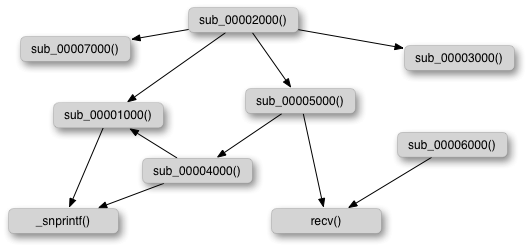
\includegraphics[scale=.40]{images/ida/cfg_call_graph.png}}
    \end{center}
\end{frame}

\begin{frame}[t]
    \frametitle{Control Flow Graphs}
    \begin{columns}
        \column{.6\textwidth}
            \begin{itemize}
                \item Functions can be visualized as graphs
                    \begin{itemize}
                        \item Basic blocks represented as nodes
                        \item Branches represented as edges
                    \end{itemize}
            \end{itemize}
            \begin{center}
                \uncover{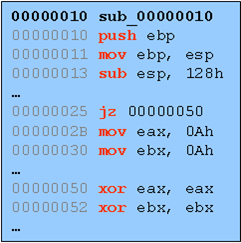
\includegraphics[scale=.30]{images/ida/cfg_deadlisting.png}}
            \end{center}
            \begin{itemize}
                \item Useful for viewing of execution paths
            \end{itemize}
        \column{.4\textwidth}
            \begin{uncoverenv}
                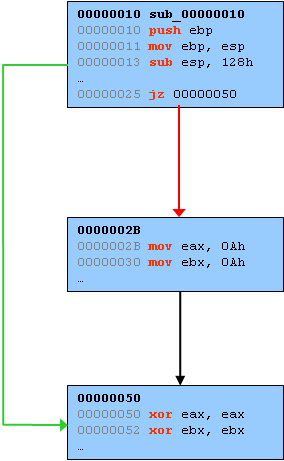
\includegraphics[scale=.40]{images/ida/cfg_graph.png}
            \end{uncoverenv}
    \end{columns}
\end{frame}


\subsection{Overview of Views}
\begin{frame}
    \frametitle{Disassembly View}
    \begin{itemize}
        \item View disassembly, stack offsets, cross refs, strings refs...
        \item Set breakpoints, change names, apply structures edit functions...
    \end{itemize}
    \begin{center}
        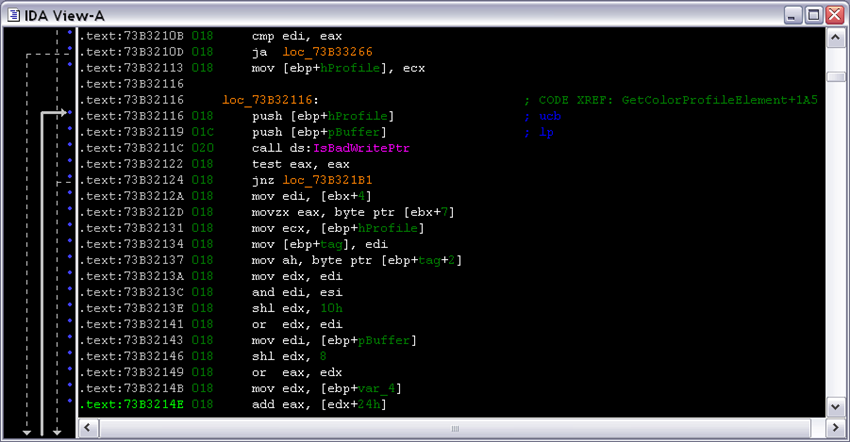
\includegraphics[scale=.75]{images/ida/disasm_view.png}
    \end{center}
\end{frame}

\begin{frame}
    \frametitle{Navigator Band}
    \begin{itemize}
        \item Colorized view of the loaded binary
    \end{itemize}
    \begin{center}
        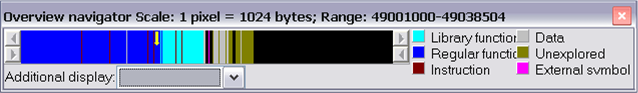
\includegraphics[scale=.50]{images/ida/navigator_band.png} \\
    \end{center}
    \tip{Bands of code that lie interlaced within library functions are probably unrecognized library routines.}
\end{frame}

\begin{frame}
    \frametitle{Messages Window}
    \begin{itemize}
        \item Contains informational messages from IDA
        \item Output from plug-ins
        \item Output from command bar
    \end{itemize}
    \begin{center}
        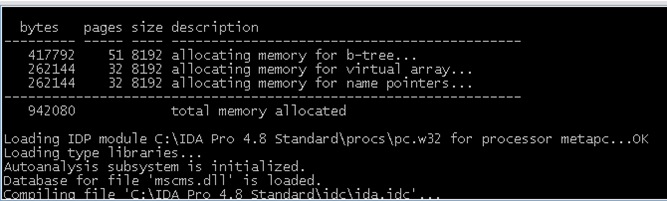
\includegraphics[scale=.50]{images/ida/messages_window.png}
    \end{center}
\end{frame}

\begin{frame}
    \frametitle{Hex View}
    \begin{itemize}
        \item Hex dump of binary
        \item Can be synchronized with disassembly view
    \end{itemize}
    \begin{center}
        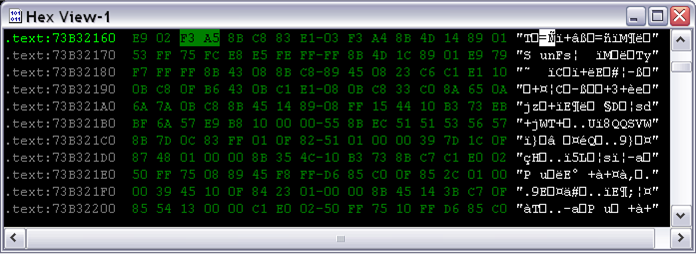
\includegraphics[scale=.60]{images/ida/hex_view.png}
    \end{center}
\end{frame}

\begin{frame}
    \frametitle{Function List}
    List of all functions defined in the current binary
    \begin{center}
        \begin{scriptsize}
        \begin{tabular}{|l|l|}                                                             \hline
            \cellcolor{lightblue}R &  Function returns to caller                           \\ \hline
            \cellcolor{lightblue}F &  Far function                                         \\ \hline
            \cellcolor{lightblue}L &  Library function                                     \\ \hline
            \cellcolor{lightblue}S &  Static Function                                      \\ \hline
            \cellcolor{lightblue}B &  EBP based frame                                      \\ \hline
            \cellcolor{lightblue}T &  Function has type information                        \\ \hline
            \cellcolor{lightblue}= &  Frame pointer is equal to the initial stack pointer  \\ \hline
        \end{tabular}
        \end{scriptsize}
    \end{center}
    \begin{center}
        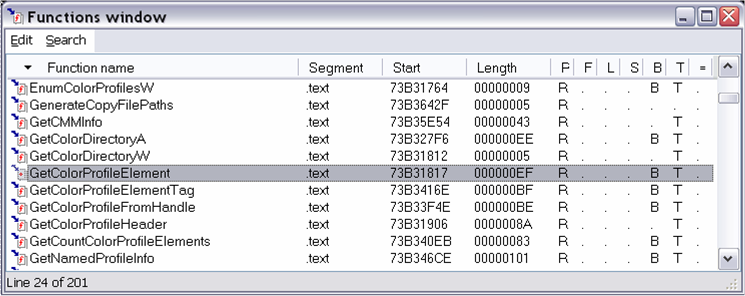
\includegraphics[scale=.50]{images/ida/function_list.png}
    \end{center}
\end{frame}

\begin{frame}
    \frametitle{Names / Symbols List}
    \begin{center}
        \begin{scriptsize}
        \begin{tabular}{|l|l|}                             \hline
            \cellcolor{lightblue}L &  Library function  \\ \hline
            \cellcolor{lightblue}F &  Regular function  \\ \hline
            \cellcolor{lightblue}C &  Instruction       \\ \hline
            \cellcolor{lightblue}A &  ASCII string      \\ \hline
            \cellcolor{lightblue}D &  Data              \\ \hline
            \cellcolor{lightblue}E &  Imported name     \\ \hline
        \end{tabular}
        \end{scriptsize}
    \end{center}
    \begin{center}
        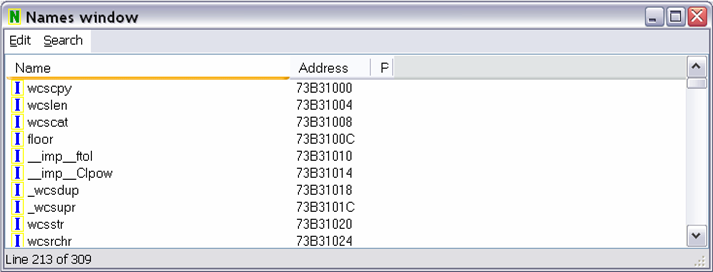
\includegraphics[scale=.50]{images/ida/names_list.png}
    \end{center}
\end{frame}

\begin{frame}
    \frametitle{Imports List}
    \begin{columns}[t]
        \column{.5\textwidth}
            \begin{itemize}
                \item View imported libraries
                \item View imported API
                \item Search
                \item You can make an educated guess of the capabilities and functionality simply by analyzing the import table
            \end{itemize}
        \column{.5\textwidth}
            \begin{center}
                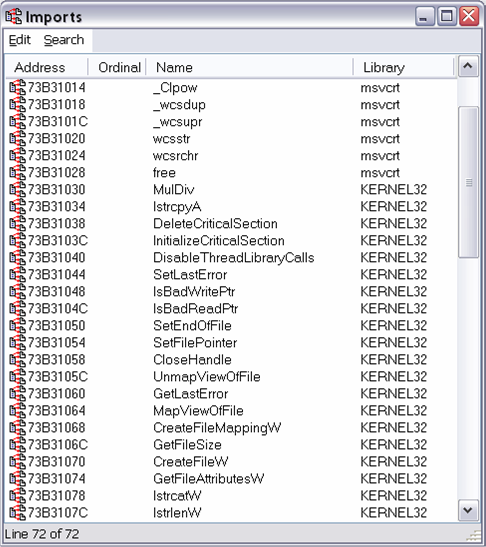
\includegraphics[scale=.50]{images/ida/imports_list.png}
            \end{center}
    \end{columns}
\end{frame}

\begin{frame}
    \frametitle{Strings List}
    \begin{itemize}
        \item View and search the complete list of discovered strings
        \item Take a look at the string list from below. Is it obvious to anyone that some strings are encoded?
    \end{itemize}
    \begin{center}
        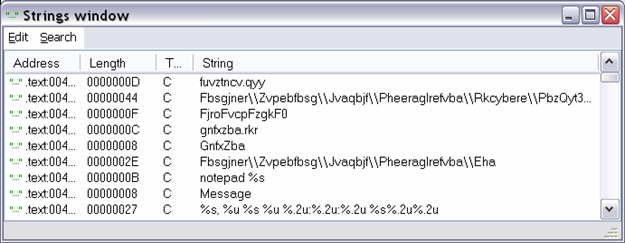
\includegraphics[scale=.85]{images/ida/strings_list.png}
    \end{center}
\end{frame}

\begin{frame}
    \frametitle{Notepad}
    \begin{itemize}
        \item Useful for jotting down notes / comments
        \item Saved in your IDB
    \end{itemize}
    \begin{center}
        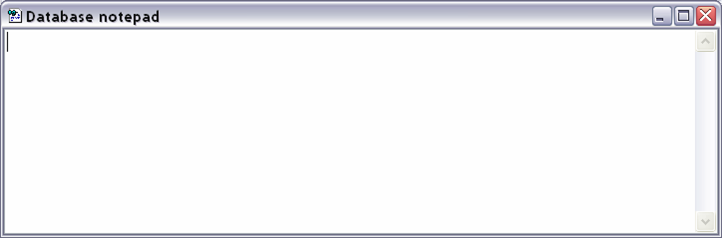
\includegraphics[scale=.50]{images/ida/notepad.png}
    \end{center}
\end{frame}

\begin{frame}
    \frametitle{Debugger}
    \begin{itemize}
        \item Worth mentioning
        \item Personally, I think it's hideous
        \item Key benefits
            \begin{itemize}
                \item Can utilize the power of IDC on breakpoints
                \item Powerful plug-in API
                \item Excellent disassembly base of course
            \end{itemize}
        \item On another note, it is good for ARM (Pocket PC) debugging
            \pedbullet{Pedram's new hobby}
    \end{itemize}
\end{frame}


\subsection{Driving IDA}
\begin{frame}
    \frametitle{Renaming Variables}
    Use the \alert{N} key to rename the argument \\
    \begin{center}
        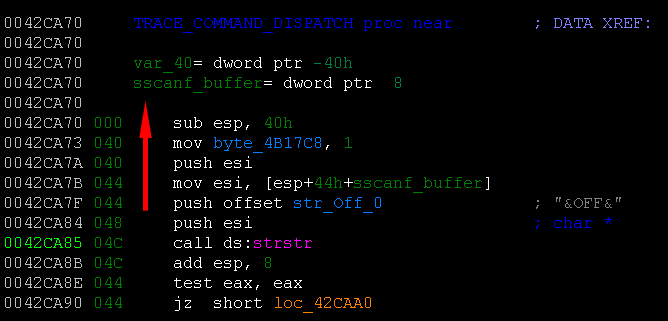
\includegraphics[scale=.50]{images/ida/renaming_variables.png} \\
    \end{center}
\end{frame}

\begin{frame}
    \frametitle{Navigating the Dead Listing}
    \begin{itemize}
        \item CTRL+UP/DOWN to scroll without losing highlight
        \item CTRL+LEFT/RIGHT to jump between items
        \item SHIFT+ENTER to highlight the current item
        \item ALT+UP/DOWN to find the last/next occurrence of the current item
    \end{itemize}
\end{frame}

\begin{frame}
    \frametitle{Marking Positions}
    \begin{itemize}
        \item ALT-M mark position
        \item CTRL-M jump to marked position
        \item To clear marks:
            \pedbullet{Jump $\rightarrow$ Clear mark, then select the mark to erase}
    \end{itemize}
\end{frame}

\begin{frame}
    \frametitle{Cross References}
    \begin{itemize}
        \item Using the Names Window, double click on an API call that you want to find in the target program.  This will highlight the call in the jump table within the disassembly window
        \item Now click on the cross-references button.  This will bring up a cross-references window
        \item By double clicking on the XREF, you will bring focus to the line of code that is making the call
        \item Shortcuts
            \pedbullet{X show all XREFs to operand}
            \pedbullet{CTRL+X show all XREFs to current EA}
    \end{itemize}
\end{frame}

\begin{frame}
    \frametitle{Forward and Backward Navigation}
    \begin{itemize}
        \item By double clicking or highlighting and pressing return, you can follow a XREF directly.
        \item Sometimes multiple XREFs will be shown in the deadlisting
        \item If you have followed multiple XREFs you can navigate back through your XREF history by pressing ESC.
        \item You can navigate forward through your XREF history by pressing CTRL+Enter
        \item Using the arrow keys, the ENTER key, and the ESC key, you can navigate the disassembly view quickly.
    \end{itemize}
\end{frame}


\subsection{Customizations}
\begin{frame}
    \frametitle{Overview}
    \begin{itemize}
        \item Toolbars
        \item Custom desktops
        \item Color palette
            \pedbullet{IDA Pro$\backslash$Customizations$\backslash$IDA Color Palette.reg}
        \item Others (next couple of slides)
            \pedbullet{IDA.CFG}
            \pedbullet{IDAGUI.CFG}
            \pedbullet{IDC scripts and hotkeys (IDA.IDC)}
    \end{itemize}
\end{frame}

\begin{frame}[fragile]
    \frametitle{IDA.CFG}
    \begin{semiverbatim}
        ASCII_PREFIX      = "str."
        MAX_NAMES_LENGTH  = 128
        NameChars         = "$?@>"
        SHOW_XREFS        = 200
        SHOW_BASIC_BLOCKS = YES
        SHOW_SP           = YES
        MangleChars       = "$:?([.)] "
    \end{semiverbatim}
\end{frame}

\begin{frame}[fragile]
    \frametitle{IDAGUI.CFG}
    \begin{semiverbatim}
        HELPFILE              = "c:\\OPS.HLP"
        DISPLAY_PATCH_SUBMENU = YES
        DISPLAY_COMMAND_LINE  = YES
        "ChartXrefsTo"        = "Ctrl-Shift-T"
        "ChartXrefsFrom"      = "Ctrl-Shift-F"
    \end{semiverbatim}
\end{frame}

\begin{frame}[fragile]
    \frametitle{IDA.IDC}
    \begin{semiverbatim}
#include <pedram_function_tagger.idc>
#include <pedram_jump_to_func_top.idc>
#include <pedram_export_disassembly.idc>
#include <pedram_assign_color.idc>

AddHotkey("Ctrl-Shift-X",    "export_disassembly");
AddHotkey("Ctrl-Shift-J",    "jump_to_func_top");
AddHotkey("Ctrl-Shift-Enter","track_follow");
AddHotkey("Ctrl-Shift-N",    "track_name");
AddHotkey("Ctrl-Shift-A",    "hotkey_assign_color");
AddHotkey("Ctrl-Alt-A",      "hotkey_deassign_color");
AddHotkey("Ctrl-Shift-B",    "hotkey_assign_block_color");
AddHotkey("Ctrl-Shift-D",    "hotkey_deassign_block_color");
    \end{semiverbatim}
\end{frame}

\begin{frame}
    \frametitle{Plugins}
    \begin{itemize}
        \item There are a number of plug-ins available
        \item For starters, install pGRAPH.plw
            \pedbullet{Copy it to \%IDA\%$\backslash$plugins}
        \item Use ALT+3 to launch the plug-in
        \item For those of you who are interested, see the next slides for instructions on installing IDA Sync
    \end{itemize}
\end{frame}

\begin{frame}
    \frametitle{Exercise}
    \begin{itemize}
        \item Customize your IDA environment
        \item Install IDA Python and other plug-ins of choice
        \item Use shortcuts!
            \pedbullet{See CD$\backslash$IDA Pro$\backslash$IDA Pro Shortcut Keys Quick Reference.pdf}
    \end{itemize}
\end{frame}


\section{OllyDbg}
\subsection{Overview}
\begin{frame}
    \frametitle{Introduction to OllyDbg}
    \begin{itemize}
        \item Freeware
        \item Contains a lot of \emph{cracker friendly} features
        \item Pluggable through a multitude of languages
        \item Scriptable through OllyScript
        \item Contains a powerful disassembler
            \pedbullet{Also available as a library}
    \end{itemize}
\end{frame}

\begin{frame}
    \frametitle{Learning Curve}
    \begin{itemize}
        \item Very daunting on first launch
        \item There are tons of \emph{hidden} features
            \pedbullet{I am still finding new ones}
        \item Fortunately there is excellent documentation
        \item The best way to learn however ...
            \begin{itemize}
                \item Open something in OllyDbg
                \item Play around with the various features
                \item Explore the various windows
                \item Customize your environment with the features you will be using
            \end{itemize}
    \end{itemize}
\end{frame}

\subsection{Overview of Views}
\begin{frame}
    \frametitle{CPU Main Window}
    \begin{center}
        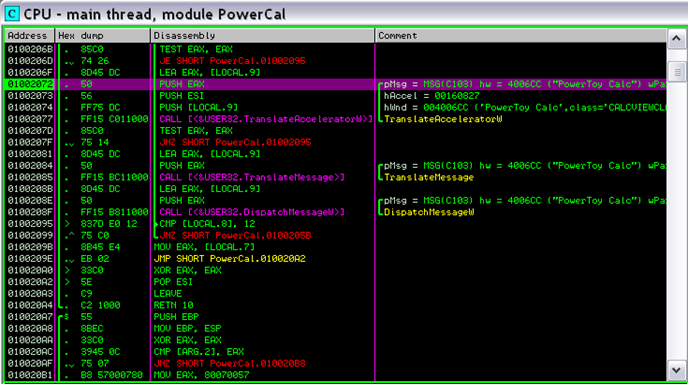
\includegraphics[scale=.75]{images/olly/cpu.png} \\
    \end{center}
    \begin{itemize}
        \item Comment-able disassembly
        \item Argument enumeration
        \item Smart de-referencing
    \end{itemize}
\end{frame}

\begin{frame}
    \frametitle{CPU Registers}
    \begin{columns}[T]
        \column{.5\textwidth}
            \begin{itemize}
                \item Editable register values
                \item CPU flags
                \item Smart de-referencing
                \item Floating point, MMX, 3DNow! Support
                \item Follow in stack/dump shortcuts
            \end{itemize}
        \column{.5\textwidth}
            \begin{center}
                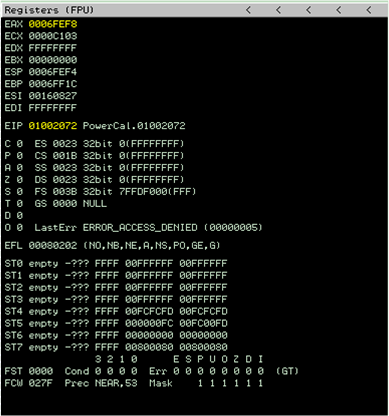
\includegraphics[scale=.45]{images/olly/cpu_registers.png}
            \end{center}
    \end{columns}
\end{frame}

\begin{frame}
    \frametitle{CPU Stack}
    \begin{columns}[T]
        \column{.5\textwidth}
            \begin{itemize}
                \item Editable
                \item Lockable
                \item View relative to ESP/EBP
                \item Smart de-referencing
                \item SEH chain
                \item Saved frames
                \item ASCII/Unicode dump
            \end{itemize}
        \column{.5\textwidth}
            \begin{center}
                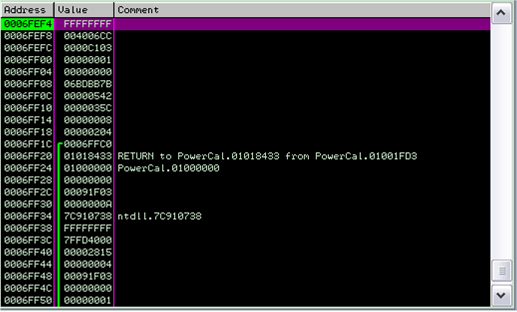
\includegraphics[scale=.60]{images/olly/cpu_stack.png}
            \end{center}
    \end{columns}
\end{frame}

\begin{frame}
    \frametitle{CPU Dump}
    \begin{columns}[T]
        \column{.5\textwidth}
            \begin{itemize}
                \item Unique and handy OllyDbg feature
                \item Multiple view types: hex, text, disassembly, long pointers, PE header and it's extensible with plug-ins (see SPECFUNC)
            \end{itemize}
        \column{.5\textwidth}
            \begin{center}
                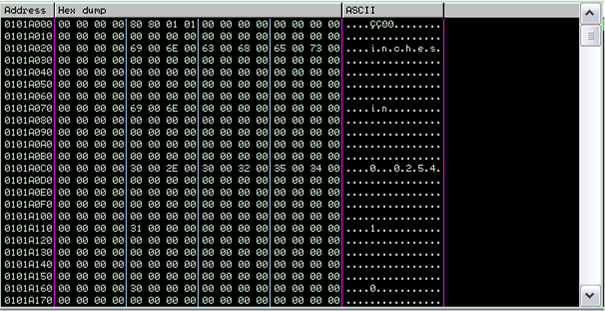
\includegraphics[scale=.60]{images/olly/cpu_dump.png}
            \end{center}
    \end{columns}
\end{frame}

\begin{frame}
    \frametitle{Log Window}
    \begin{center}
        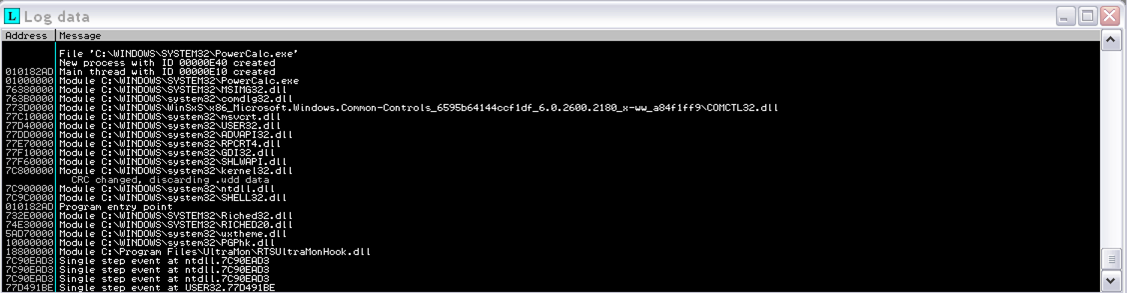
\includegraphics[scale=.60]{images/olly/log.png} \\
    \end{center}
    \begin{itemize}
        \item Debugger / plug-in output messages
            \pedbullet{Breakpoint / log breakpoint output}
            \pedbullet{Access violations}
            \pedbullet{Etc...}
        \item Debuggee messages through OutputDebugString() API
    \end{itemize}
\end{frame}

\begin{frame}
    \frametitle{Call Stack}
    \begin{center}
        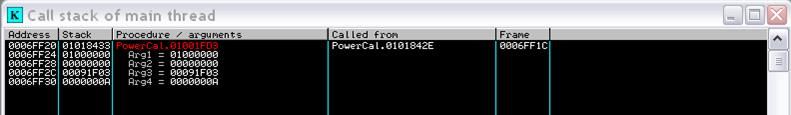
\includegraphics[scale=.50]{images/olly/call_stack.png} \\
    \end{center}
    \begin{itemize}
        \item Collapsible with arguments
        \item Stack walking is not an exact science, especially when standard EBP based frames are not used.
        \item Olly is pretty smart about it
    \end{itemize}
\end{frame}

\begin{frame}
    \frametitle{Threads}
    \begin{center}
        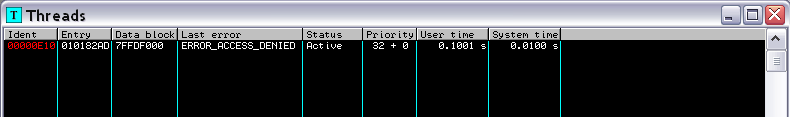
\includegraphics[scale=.75]{images/olly/threads.png} \\
    \end{center}
    \begin{itemize}
        \item List of threads in current process
    \end{itemize}
    \begin{uncoverenv}
        \tip{When attempting to determine which thread processes an input, say for example network packets, fire off some packets forcing the process to work and watch the User/System time columns.}
    \end{uncoverenv}
\end{frame}

\begin{frame}
    \frametitle{Executable Modules}
    \begin{center}
        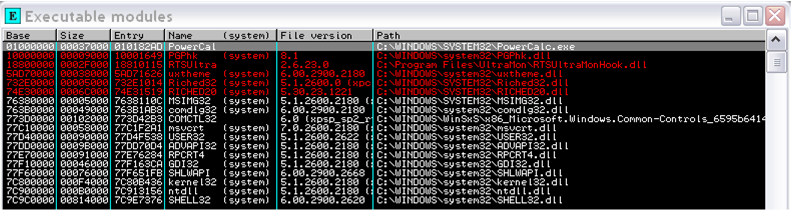
\includegraphics[scale=.60]{images/olly/executable_modules.png} \\
    \end{center}
    \begin{itemize}
        \item List of modules currently loaded in the debuggee's process space
        \item The Name column contains the �hidden� system tag (run traces)
        \item Ctrl+N to view exported names
        \item Breakpoints / log breakpoints can be set
        \item Olly knows the argument types for a lot of standard API calls
    \end{itemize}
\end{frame}

\begin{frame}
    \frametitle{Memory Map}
    \begin{columns}[T]
        \column{.5\textwidth}
            \begin{itemize}
                \item Searchable full-range memory map
                \item Stack is tagged, heaps are not
                \item OllyDbg Heap Vis plug-in allows you to list, search and visualize the heap
            \end{itemize}
        \column{.5\textwidth}
            \begin{center}
                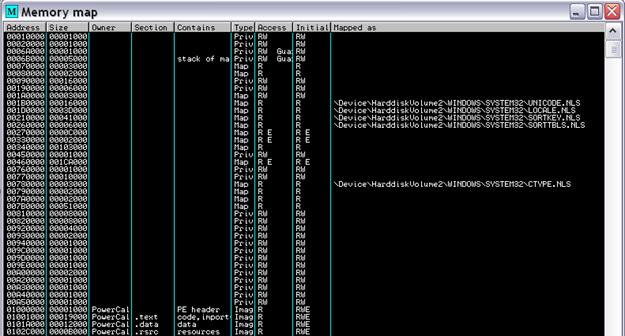
\includegraphics[scale=.60]{images/olly/memory_map.png}
            \end{center}
    \end{columns}
\end{frame}

\begin{frame}
    \frametitle{Breakpoints}
    \begin{center}
        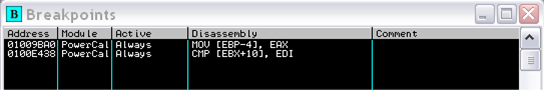
\includegraphics[scale=.50]{images/olly/breakpoints.png} \\
    \end{center}
    \begin{itemize}
        \item OllyDbg supports regular breakpoints, conditional breakpoints and conditional log breakpoints
        \item Breakpoints set in the main module are persistent across debugger sessions.
        \item OllyDbg BP Manager plug-in allows you to import/export breakpoints lists
        \item You can use the BP Manager to automatically load breakpoints on module load
    \end{itemize}
\end{frame}

\begin{frame}
    \frametitle{Bookmarks}
    \begin{center}
        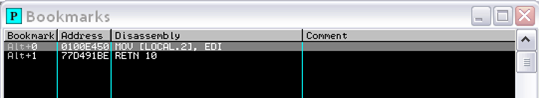
\includegraphics[scale=.50]{images/olly/bookmarks.png} \\
    \end{center}
    \begin{itemize}
        \item Bookmarking is provided by a plug-in bundled with OllyDbg
        \item Simply set and quick jump to various locations
        \item Identical to "marks" in IDA
    \end{itemize}
\end{frame}

\begin{frame}
    \frametitle{SEH Chain}
    \begin{columns}[T]
        \column{.5\textwidth}
            \begin{itemize}
                \item Unique OllyDbg feature
                \item Does not show the vector based exception handling chain
            \end{itemize}
        \column{.5\textwidth}
            \begin{center}
                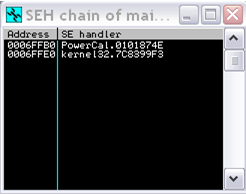
\includegraphics[scale=.50]{images/olly/seh_chain.png}
            \end{center}
    \end{columns}
\end{frame}

\begin{frame}
    \frametitle{Watch Expressions}
    \begin{columns}[T]
        \column{.5\textwidth}
            \begin{itemize}
                \item OllyDbg supports an expression language allowing the user to create real-time watches
                \item Useful when tracking changes to complex data types
            \end{itemize}
        \column{.5\textwidth}
            \begin{center}
                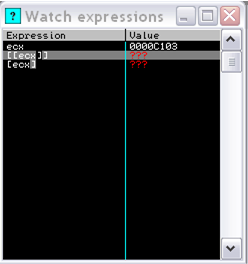
\includegraphics[scale=.50]{images/olly/watch_expressions.png}
            \end{center}
    \end{columns}
\end{frame}

\begin{frame}
    \frametitle{Handles}
    \begin{center}
        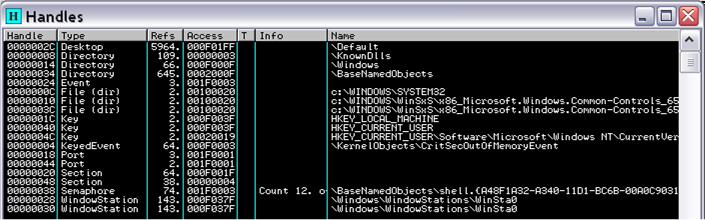
\includegraphics[scale=.50]{images/olly/handles.png} \\
    \end{center}
    \begin{itemize}
        \item List of open handles
        \item Tag / untag
            \pedbullet{Not sure entirely what this is for.}
    \end{itemize}
\end{frame}

\begin{frame}
    \frametitle{Plug-ins}
    \begin{block}{Fact}
    OllyDbg has excellent plug-in support and great API documentation. Much better than IDA.
    \end{block}
    \begin{itemize}
        \item GODUP
            \pedbullet{Load labels and comments from IDA}
        \item OllyDump
            \pedbullet{Dump the running process to disk, IAT rebuilding (malware purposes)}
        \item Heap Vis
            \pedbullet{Enumerate and search process heap}
        \item Breakpoint Manager
            \pedbullet{Import / export breakpoint sets}
        \item De-Attach Helper
            \pedbullet{Adds detach support and WinDbg similar "attach to last" functionality}
    \end{itemize}
\end{frame}


\subsection{Driving OllyDbg}
\begin{frame}
    \frametitle{Hot Keys}
    \begin{center}
        \begin{tabular}{l l}
            \uncover{\cellcolor{lightblue} F9         & \cellcolor{lightblue}Execute debuggee         \\}
            \uncover{                      CTRL + F9  & Execute until return                          \\}
            \uncover{\cellcolor{lightblue} ALT + F9   & \cellcolor{lightblue}Execute until user code  \\}
            \uncover{                      F12        & Pause                                         \\}
            \uncover{\cellcolor{lightblue} F7         & \cellcolor{lightblue}Step into                \\}
            \uncover{                      F8         & Step over                                     \\}
            \uncover{\cellcolor{lightblue} F2         & \cellcolor{lightblue}Set / clear breakpoint   \\}
            \uncover{                      CTRL + G   & Follow expression                             \\}
            \uncover{\cellcolor{lightblue} any key    & \cellcolor{lightblue}Add comment              \\}
            \uncover{                      :          & Add label                                     \\}
        \end{tabular}
    \end{center}
\end{frame}

\begin{frame}
    \frametitle{Following Expressions}
    \begin{center}
        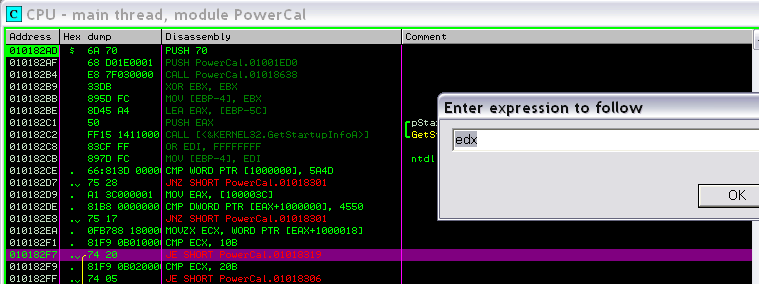
\includegraphics[scale=.25]{images/olly/follow_expression.png} \\
    \end{center}
    \begin{itemize}
        \item Use CTRL+G to open the \emph{follow expression} window
        \item You can specify an address, register, or the label of a function, such as recv or sprintf
    \end{itemize}
    \begin{uncoverenv}
        \tip{Sometimes you have to CTRL+G \alert{twice} in order to get it to resolve to the actual location. This appears to be a bug.}
    \end{uncoverenv}
\end{frame}

\begin{frame}
    \frametitle{Software Breakpoints}
    \begin{center}
        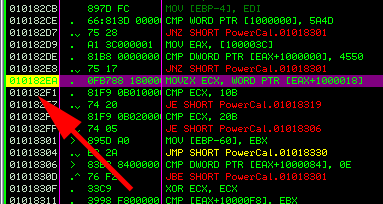
\includegraphics[scale=.50]{images/olly/set_breakpoint.png} \\
    \end{center}
    \begin{itemize}
        \item Set focus on the target instruction
        \item Hit F2 to set / unset the breakpoint
    \end{itemize}
\end{frame}

\begin{frame}
    \frametitle{Hardware Breakpoints}
    \begin{center}
        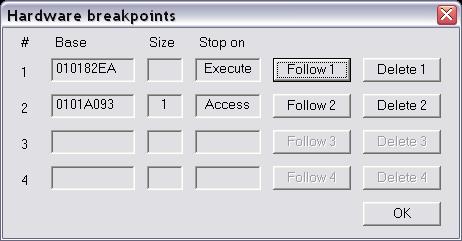
\includegraphics[scale=.30]{images/olly/hardware_breakpoints.png} \\
    \end{center}
    \begin{itemize}
        \item You get 4 hardware breakpoints
        \item CPU supported, so transparent to software
        \item Set focus on the target instruction or memory address
        \item Right click $\rightarrow$ breakpoint $\rightarrow$ hardware
        \item Three classes: access, write and execute
        \item Three sizes: byte (1), word (2), dword (4)
    \end{itemize}
\end{frame}

\begin{frame}
    \frametitle{Memory Breakpoints}
    \begin{itemize}
        \item Actually it's just memory \alert{breakpoint}, you get one
        \item OllyDbg accomplishes this task by changing the permissions of the page that contains your target address
        \item You should opt to use hardware breakpoints over this feature
        \item In case you really need a 5th on-access type breakpoint, it's there for you
    \end{itemize}
\end{frame}

\begin{frame}
    \frametitle{Enumerating Functions}
    \begin{center}
        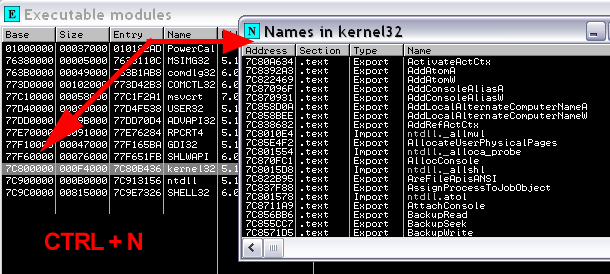
\includegraphics[scale=.40]{images/olly/enumerate_functions.png} \\
    \end{center}
    \begin{itemize}
        \item Go to the \emph{executable modules} window
        \item Highlight the DLL you are interested in
        \item Hit \alert{CTRL + N} to pull up a list of imports/exports
        \item You can hit F2 directly on this list to set breakpoints
    \end{itemize}
\end{frame}

\begin{frame}
    \frametitle{Searching}
    \begin{columns}[T]
        \column{.6\textwidth}
            \begin{itemize}
                \item One of the best OllyDbg features
                \item You can search modules, memory, stack
                \item Search for strings or commands
                \item Search for variable register commands
                \item Search for all string references
            \end{itemize}
        \column{.4\textwidth}
            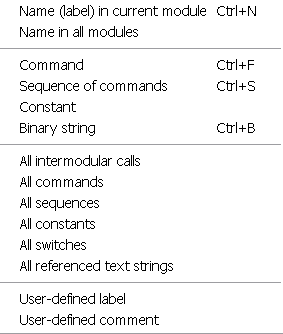
\includegraphics[scale=.40]{images/olly/search.png}
    \end{columns}
\end{frame}

\begin{frame}
    \frametitle{Run Trace and Animate}
    \begin{itemize}
        \item These features are unique to OllyDbg
        \item Animate is useful for watching loop or recursion activity
        \item Run trace is useful for all sorts of tasks
        \begin{itemize}
            \item Unfortunately run trace is extremely slow
            \item Speed was a major motivating factor in my development of alternative code coverage techniques
            \item Pedram can show you demo's of Process Stalker and PaiMei if we have time
        \end{itemize}
    \end{itemize}
\end{frame}

% included by ../header.tex

\part{Advanced Analysis}

\section{Executable (Un)Packing}
\subsection{Executable Packing}
\begin{frame}
    \frametitle{Binary Protection}
    \begin{itemize}
        \item Malware authors use both packers and crypters to reduce file size and increase analysis time
        \item Packers confuse disassembly by making code look like data
        \item A packer may contain anti-debugger/disassembler tricks such as SEH trickery and jumping into the middle of instructions
        \item A number of packers exist
            \pedbullet{PE: UPX, ASPack, tElock, yodacrypt, FSG, etc...}
            \pedbullet{ELF: UPX, BurnEye, etc...}
        \item We will create a basic packer to gain a better understanding of unpacking
    \end{itemize}
\end{frame}

\begin{frame}
    \frametitle{Packer Components}
    \begin{itemize}
        \item The original executable code of the target application must be obfuscated or encrypted
        \item When the application is launched the packer decoder routine must be executed first (entry point modification)
        \item The decoder routine must restore the original executable code
        \item The decoder routine must transfer control to the original executable code
        \item To get a better understanding of this subject we're going to manually construct a packer
    \end{itemize}
\end{frame}

\begin{frame}
    \frametitle{What Packing is Not}
    \begin{itemize}
        \item We don't consider run-time instrumented protection "packing"
            \pedbullet{Shiva}
        \item Such protection schemes do exist, but are rarely used in malware
            \pedbullet{Probably because they require compile time modifications}
    \end{itemize}
\end{frame}

\begin{frame}
    \frametitle{The Target Application}
    \begin{itemize}
        \item original\_hello.exe
            \pedbullet{Simple application written in C}
            \pedbullet{Prints "Hello World" and waits for keypress}
        \item Examine the PE structure information of the original executable:
    \end{itemize}
    \begin{center}
        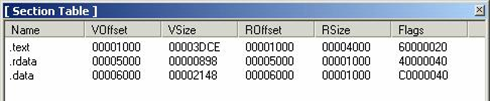
\includegraphics[scale=.50]{images/executable_packing/the_target_application.png} \\
    \end{center}
    \begin{itemize}
        \item Notice the virtual size of 0x3DCE and the raw size of 0x4000 indicating that there should be 562 bytes of slack space at the end of the .TEXT section
        \item Verify this fact with a hex editor (offset 0x4DCE)
    \end{itemize}
\end{frame}

\begin{frame}
    \frametitle{Abusing Slack Space}
    \begin{itemize}
        \item We are going to take advantage of the identified slack space by inserting our decoder stub into it
        \item PE modifications must be made
            \pedbullet{The .TEXT section must be made writable so our decoder stub can modify it}
            \pedbullet{The VSize must be increased so our decoder stub gets mapped into memory}
    \end{itemize}
    \begin{center}
        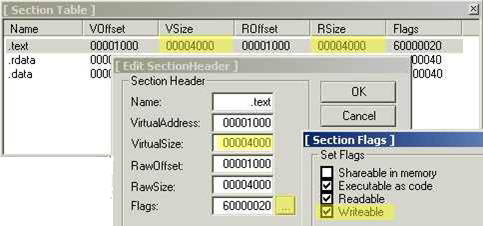
\includegraphics[scale=.40]{images/executable_packing/abusing_slack_space.png} \\
    \end{center}
\end{frame}

\begin{frame}
    \frametitle{Abusing Slack Space}
    \begin{itemize}
        \item Next, we must modify the Entry Point (EP) to point to our decoder stub. Lets set it to 0x4E00
        \item Alternative strategies for storing a decoder stub include
            \pedbullet{New sections}
            \pedbullet{Instruction gap abuse}
            \pedbullet{Entirely new PE file}
    \end{itemize}
\end{frame}

\begin{frame}[fragile]
    \frametitle{Encoding the Executable Code}
    \begin{itemize}
        \item For the purposes of this exercise we will manually encode the original executable code
        \item Simple XOR routine (VB):
    \end{itemize}
    \begin{tiny}
    \begin{semiverbatim}
        StartAt = &H1048   'Original EP
        length  = &H2D86   '3DCE - 1048 (Original VSize � Original EP)

        Open filename For Binary As file

        For i = 1 To length
            offset = StartAt + i
            Get file, offset, byte
            byte = byte Xor &HF
            Put file, offset, byte
        Next

        Close file
    \end{semiverbatim}
    \end{tiny}
    \begin{itemize}
        \item Compiled helper app: do\_opcode\_crypt.exe
    \end{itemize}
\end{frame}

\begin{frame}[fragile]
    \frametitle{Writing the Decoder Stub}
    \begin{itemize}
        \item Our binary is now ready to accept a decoder
        \item We'll write the decoder in C, compile it and then extract the byte code
    \end{itemize}
    \begin{tiny}
    \begin{semiverbatim}
        void main (void)
        \{
            int i;
            char b;

            char *buffer = 0x400000;   // imagebase
            long length  = 0xBEEF;     // length of code (placeholder)

            buffer += 0xDEAD;          // OEP offset (placeholder)

            for(i = 0; i < length; i++)
            \{
                b = buffer[i];
                b = b ^ 0xF;
                buffer[i] = b;
            \}

            _asm jmp buffer
        \}
    \end{semiverbatim}
    \end{tiny}
\end{frame}

\begin{frame}[fragile]
    \frametitle{Converting the Decoder Stub}
    \begin{itemize}
        \item Compile the decoder stub in Visual C
        \item Set a breakpoint at the top of the code
        \item Enter the debugger with F5 and choose �goto disassembly�
        \item Disassembly excerpt:
    \end{itemize}
    \begin{tiny}
    \begin{semiverbatim}
        \alert{EB 09      }   jmp   main+43h
        \alert{8B 4D FC   }   mov   ecx, dword ptr [ebp-4]
        \alert{83 C1 01   }   add   ecx, 1
        \alert{89 4D FC   }   mov   dword ptr [ebp-4], ecx
        \alert{8B 55 FC   }   mov   edx, dword ptr [ebp-4]
        \alert{3B 55 F0   }   cmp   edx, dword ptr [ebp-10h]
        \alert{7D 22      }   jge   main+6Dh
        \alert{8B 45 F4   }   mov   eax, dword ptr [ebp-0Ch]
        \alert{03 45 FC   }   add   eax, dword ptr [ebp-4]
        \alert{8A 08      }   mov   cl, byte ptr [eax]
        \alert{88 4D F8   }   mov   byte ptr [ebp-8], cl
        \alert{0F BE 55 F8}   movsx edx, byte ptr [ebp-8]
    \end{semiverbatim}
    \end{tiny}
\end{frame}

\begin{frame}[fragile]
    \frametitle{Inserting the Decoder Stub}
    \begin{itemize}
        \item Copy out the hex bytes (\alert{remove newlines}):
    \end{itemize}
    \begin{tiny}
    \begin{semiverbatim}
        C745F400004000C745F0EFBE00008B45F405ADDE00008945F4C745FC
        00000000EB098B4DFC83C101894DFC8B55FC3B55F07D228B45F40345
        FC8A08884DF80FBE55F883F20F8855F88B45F40345FC8A4DF88808EB
        CDFF65F4
    \end{semiverbatim}
    \end{tiny}
    \begin{itemize}
        \item Open the target application in WinHex
        \item Highlight offset 0x4E00, hit Ctrl+B (write clipboard) and select �ASCII Hex�
        \item The final step is to modify the placeholders with real values. Remember, little endian
    \end{itemize}
    \begin{tiny}
    \begin{semiverbatim}
        Offset      0  1  2  3
        00004E10   .. .. AD DE    (DEAD)
        00004E10   .. .. 48 10    (1048)

        Offset      0  1  2  3  4  5  6  7  8  9  A  B
        00004E00   .. .. .. .. .. .. .. .. .. .. EF BE  (BEEF)
        00004E00   .. .. .. .. .. .. .. .. .. .. 86 2D  (2D86)
    \end{semiverbatim}
    \end{tiny}
\end{frame}

\begin{frame}[fragile]
    \frametitle{Watch it in Action}
    \begin{itemize}
        \item Load the modified file in OllyDbg
        \item Look at the original EP and verify that it's not recognized as executable code
        \item Set a breakpoint at the end of the decoder stub
    \end{itemize}
    \begin{tiny}
    \begin{semiverbatim}
        00404E53  EB CD    JMP SHORT final.00404E22
        00404E55  FF65 F4  \alert{JMP [EBP-C]}               ; final.00401048
    \end{semiverbatim}
    \end{tiny}
    \begin{itemize}
        \item Hit F9 to run through the decoder
        \item Look at the original EP again
            \pedbullet{Right click "Analysis$\rightarrow$Analyze code" (Ctrl-A)}
    \end{itemize}
\end{frame}

\begin{frame}
    \frametitle{Exercise}
    \begin{itemize}
        \item Create your own packer
        \item Follow these high-level steps:
            \pedbullet{Copy original\_hello.exe to pe\_modified\_hello.exe}
            \pedbullet{Modify pe\_modified\_hello.exe with LordPE}
            \pedbullet{Run do\_opcode\_crypt.exe to create crypted.exe}
            \pedbullet{Insert the decoder stub into crypted.exe}
            \pedbullet{Verify crypted.exe works}
            \pedbullet{Verify crypted.exe is indeed "crypted"}
        \item Some shortcuts were made for you
    \end{itemize}
\end{frame}


\subsection{Executable Unpacking}
\begin{frame}[fragile]
    \frametitle{Detecting Packed Executables}
    \begin{itemize}
        \item Entry Point (EP) lies outside of .TEXT section
        \item .TEXT section is writable
        \item Sections with 0 size
        \item Limited imports
        \item No strings
        \item Entropy (compressibility of bytes)
            \pedbullet{Ghetto check: compression}
    \end{itemize}
    \begin{tiny}
    \begin{semiverbatim}
        \$ cat calc.exe | gzip -v > /dev/null
         55.8%

        \$ cat calc-upx.exe | gzip -v > /dev/null
         24.9%

        \$ cat calc-aspack.exe | gzip -v > /dev/null
         25.2%
    \end{semiverbatim}
    \end{tiny}
\end{frame}

\begin{frame}
    \frametitle{The Easy Way: PEiD}
    \begin{itemize}
        \item Has a multitude of signatures (somewhat outdated)
        \item You can add your own (many publicly exist)
        \item Entropy detection
        \item Generic detection
        \item Generic unpacking with intelligent OEP detection
    \end{itemize}
    \begin{center}
        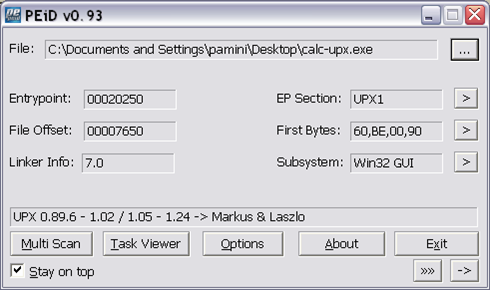
\includegraphics[scale=.50]{images/executable_packing/peid.png} \\
    \end{center}
\end{frame}

\begin{frame}
    \frametitle{Methodologies}
    \begin{itemize}
        \item There are three basic methodologies to unpacking
        \item Post execution analysis
            \pedbullet{An easy and generic approach}
            \pedbullet{Most dangerous}
        \item Controlled run-time analysis
            \pedbullet{More difficult to do}
            \pedbullet{More control / less dangerous}
            \pedbullet{PEiD attempts to automate this, but we don't trust anything automated}
        \item Static analysis / basic emulation
            \pedbullet{Most difficult to do}
            \pedbullet{Safe}
    \end{itemize}
\end{frame}

\begin{frame}
    \frametitle{Post Execution Analysis}
    \begin{itemize}
        \item Launch the packed binary in a controlled environment
        \item The decoder stub will run leaving an unpacked copy of the binary in memory
        \item Dump the running process to disk
            \pedbullet{OllyDbg +OllyDump}
            \pedbullet{ProcDump}
            \pedbullet{Etc...}
        \item Fix the Import Address Table (IAT) and analyze (more on this later)
    \end{itemize}
\end{frame}

\begin{frame}
    \frametitle{Controlled Run-Time Analysis}
    \begin{itemize}
        \item Load the packed binary in a debugger
        \item Single step through the decoder stub until a transfer is made to the Original Entry Point (OEP)
    \end{itemize}
    \begin{columns}
        \column{.5\textwidth}
            \begin{itemize}
                \item Dump the running process to disk
                    \pedbullet{OllyDbg +OllyDump}
                    \pedbullet{Etc...}
                \item Fix the Import Address Table (IAT) and analyze (more on this later)
            \end{itemize}
        \column{.5\textwidth}
            \begin{center}
                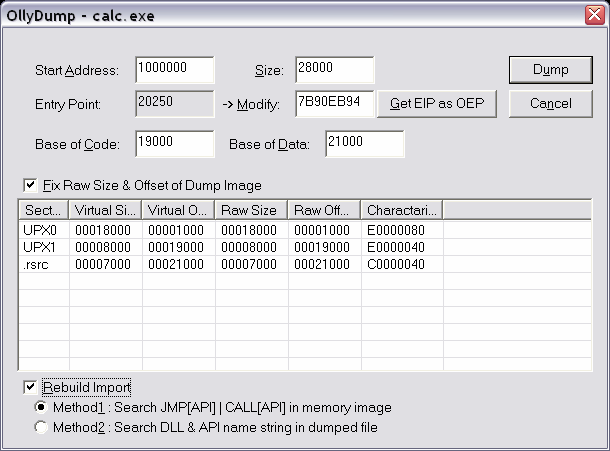
\includegraphics[scale=.50]{images/executable_packing/ollydump.png} \\
            \end{center}
    \end{columns}
\end{frame}

\begin{frame}
    \frametitle{IAT Reconstruction}
    \begin{itemize}
        \item Why do we want to rebuild the IAT?
            \pedbullet{Analyzing a malicious binary without symbols is burdensome}
        \item There are a number of approaches to IAT reconstruction
    \end{itemize}
    \begin{columns}
        \column{.5\textwidth}
            \begin{itemize}
                \item We will cover three approaches
                    \pedbullet{OllyDump}
                    \pedbullet{ImportRec}
                    \pedbullet{IDCDumpFix}
                \item Depending on the target, one approach may work better than another
            \end{itemize}
        \column{.5\textwidth}
            \begin{center}
                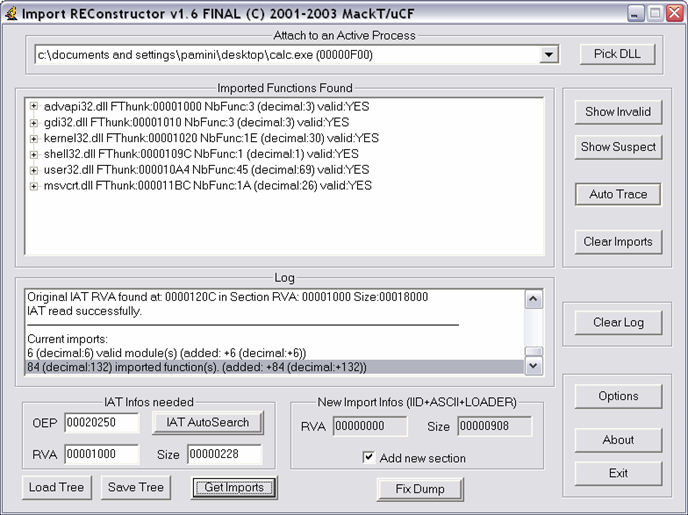
\includegraphics[scale=.50]{images/executable_packing/importrec.png} \\
            \end{center}
    \end{columns}
\end{frame}

\begin{frame}
    \frametitle{Static Analysis / Basic Emulation}
    \begin{columns}
        \column{.5\textwidth}
            \begin{itemize}
                \item If possible, such as with UPX, manually unpack the binary with the relevant unpacker
                \item Process the binary with an emulator such as Chris Eagle's x86-emu plug-in
                \item Single step through the decoder stub until the IDA database is completely decoded
            \end{itemize}
        \column{.5\textwidth}
            \begin{center}
                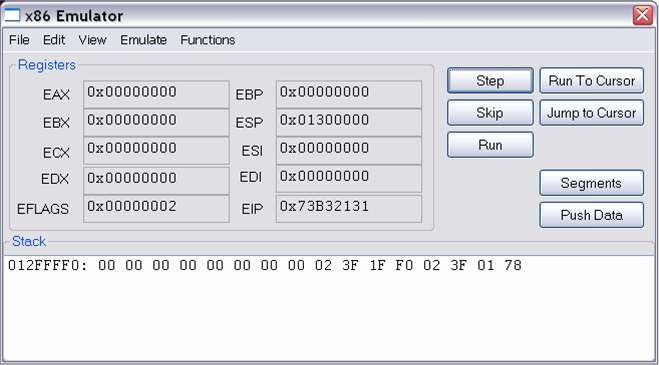
\includegraphics[scale=.50]{images/executable_packing/x86-emu.png} \\
            \end{center}
    \end{columns}
\end{frame}

\begin{frame}
    \frametitle{Exercises}
    \begin{itemize}
        \item Examine the PE structure of calc*.exe
        \item Unpack calc-aspack.exe using post execution analysis
        \item Unpack calc-upx.exe using controlled run-time analysis
        \item Unpack the custom packed file from the previous exercise using x86-emu
        \item For the daring, unpack calc-aspack.exe using controlled run-time analysis. Watch for the anti-disasm trickery at EP.
        \item Rebuild IATs using various techniques and compare.
        \item See the following files for hints ONLY if you get stuck
            \pedbullet{OpenRCE ASPack Notes.txt}
            \pedbullet{OpenRCE UPX Notes.txt}
    \end{itemize}
\end{frame}

\begin{frame}
    \frametitle{Automation Exercises}
    \begin{itemize}
        \item Automate the process of dumping and reconstruction with pydbg and pefile
        \item Attach to a running process
        \item Preprocess common system DLLs and harvest the default addresses of the exported symbols
        \item Scan and dump the address space while also looking for possible pointers to the DLL's exported symbols' addresses
        \item Generate IDAPython/IDC output that can be loaded directly into IDA to recover the symbols in the loaded dump
    \end{itemize}
\end{frame}


\begin{frame}
    \frametitle{Original Entry Point (OEP) Discovery Techniques}
    \begin{itemize}
        \item Graph analysis
        \item PUSH/POP trick
        \item Common APIs
        \item Markov chains on instruction patterns
        \item Taint analysis
    \end{itemize}
\end{frame}


\subsection{Packer Usage Statistics}
\begin{frame}
    \frametitle{The Corpus}
    \begin{itemize}
        \item Had just under 50.000 malware samples lying around
        \item Ran them through a beta of \emph{pefile} which employs \emph{PEiD}'s packer signature database
        \item In around 42\% of the files no packer could be found
        \item In the remaining (~58\%) of the files over 200 packers and compilers were identified
    \end{itemize}
\end{frame}

\begin{frame}
    \frametitle{Most Frequently Used}
    \begin{itemize}
        \item The most frequently occurring packer among the samples, \emph{UPX}, would probably not surprise anyone that has been looking at malware for a while.
        \item It appeared in around 13\% of the samples.
        \item \emph{Mew}, \emph{PeCompact}, \emph{ASPack}, \emph{FSG}, \emph{y0da's Crypter}, \emph{Armadillo} and other versions of UPX took the next places.
    \end{itemize}
\end{frame}

\begin{frame}
    \frametitle{Most Common Packers}
        \begin{center}
            \pgfimage[height=7cm]{images/executable_packing/packer_stats_pie_chart}
        \end{center}
\end{frame}


\begin{frame}
    \frametitle{The Long Tail}
    \begin{itemize}
        \item Reverse engineers and analysts have to confront a large variety of packers and their modified versions
        \item PEiD's largest databases have over 2000 entries
            \pedbullet{http://www.secretashell.com/BobSoft/}
        \item The most obscure packers tend to appear with a relatively low frequency
        \item Yet, it's usually those more exotic packers, the ones incorporating fancier techniques
        \item In the future we will see more technologies aimed at generically unpacking samples (like the old SCU, or PEiD's and Procdump's methods)
    \end{itemize}
\end{frame}

\begin{frame}
    \frametitle{The Long Tail}
        \begin{center}
            \pgfimage[width=11cm]{images/executable_packing/packer_stats_bar_chart}
        \end{center}
\end{frame}




\subsection{Unpacking Traces}
\begin{frame}
    \frametitle{The Concept}
    \begin{itemize}
        \item Thought it would be cool to be able to see how unpacking happens for different packers
        \item It's as "easy" as tracing all memory writes and EIP location as the unpacker goes on its way
        \item With help of a special tool that can be achieved without worrying about packer specifics
    \end{itemize}
\end{frame}

\begin{frame}
    \frametitle{Plotting the Data}
    \begin{itemize}
        \item A subset of all the data extracted was plotted with the help of Mathematica
        \item EIP = blue
        \item Memory writes = green
        \item The address space being displayed is the one of the unpacked process, therefore it'll be the same for all packers (all traces are of \emph{Notepad.exe} being unpacked)
        \item The horizontal axis represents time (instructions executed)
        \item The vertical axis represents the address being executed or written to (it has been limited roughly to the address range of the unpacked image)
    \end{itemize}
\end{frame}

\begin{frame}
  \frametitle{UPX-1.95}
  \begin{block}{}
  \emph{UPX-1.95} is one of the most frequently used packers, it does have a good compression ratio but has no features to attempt to prevent dumping or to obfuscate the unpacking process
  \end{block}
    \begin{itemize}
        \item The unpacking code runs in a very constrained area
        \item Just decompresses all the sections at once, the slope variations come from different data being faster to decompress than other
        \item In the final pass it just fixes the \emph{IAT} to point to the \emph{DLL} functions
    \end{itemize}
\end{frame}

\begin{frame}
  \frametitle{UPX-1.95 Visualization}
  \begin{center}
    \pgfimage[height=7cm]{images/unpacking_traces/UPX-1.95}%
  \end{center}
\end{frame}

\begin{frame}
  \frametitle{AsPack 2.12}
  \begin{block}{}
  \emph{AsPack} compresses all sections and goes through a lengthy unpacking algorithm until finally writing the unpacked data to the target sections
  \end{block}
    \begin{itemize}
        \item Does not compress padding or empty section areas
        \item The actual writing of the data happens in rather tight loops
    \end{itemize}
\end{frame}

\begin{frame}
  \frametitle{AsPack 2.12 Visualization}
  \begin{center}
    \pgfimage[height=7cm]{images/unpacking_traces/ASPack_2.12}%
  \end{center}
\end{frame}

\begin{frame}
  \frametitle{FSG v2.0}
  \begin{block}{}
  \emph{FSG} is extremely simple, it simply goes though a decompression loop writing the data straight to the final destination
  \end{block}
    \begin{itemize}
        \item Differences on the slope of the memory writes data indicate different compression ratios. Redundant data is faster to decompress
        \item The \emph{EIP} (blue) is lost for a while, the reason is that it's executing outside the visible range, within \emph{DLL}s
    \end{itemize}
\end{frame}

\begin{frame}
  \frametitle{FSG v2.0 Visualization}
  \begin{center}
    \pgfimage[height=7cm]{images/unpacking_traces/FSG_v2.0}%
  \end{center}
\end{frame}

\begin{frame}
  \frametitle{Petite 2.2}
  \begin{block}{}
  \emph{Petite 2.2} is an interesting case, here we can see an instance of a multi-stage packer
  \end{block}
    \begin{itemize}
        \item Data written to the \emph{.data} section is later run
        \item It does two passes over the code section
        \item There is, as with other packers, a final pass fixing the \emph{IAT}
    \end{itemize}
\end{frame}

\begin{frame}
  \frametitle{Petite 2.2 Visualization}
  \begin{center}
    \pgfimage[height=7cm]{images/unpacking_traces/Petite_2.2}%
  \end{center}
\end{frame}

\begin{frame}
  \frametitle{tElock V0.98}
  \begin{block}{}
  \emph{tElock V0.98} is a rather complex case. Again it's possible to see a multi-stage packer
  \end{block}
    \begin{itemize}
        \item The code section is written in three passes
        \item It does not compress the \emph{.rsrc} section but just the valid data in \emph{.data}
        \item As with the \emph{FSG} packer, the EIP escapes the shown address range to go execute \emph{DLL} code
        \item It does a quick final \emph{IAT} fix-up
    \end{itemize}
\end{frame}

\begin{frame}
  \frametitle{tElock V0.98 Visualization}
  \begin{center}
    \pgfimage[height=7cm]{images/unpacking_traces/tElock_v.098}%
  \end{center}
\end{frame}

\begin{frame}
  \frametitle{Yoda's Crypter v1.3}
  \begin{block}{}
  \emph{Yoda's Crypter v1.3} is fast and straightforward
  \end{block}
    \begin{itemize}
        \item Only compresses the \emph{.text} and \emph{.data} sections
        \item Runs within a small area of code after the last section of the original binary
        \item It's also multi-stage
    \end{itemize}
\end{frame}

\begin{frame}
  \frametitle{Yoda's Crypter v1.3 Visualization}
  \begin{center}
    \pgfimage[height=7cm]{images/unpacking_traces/Yodas_Crypter_v1.3}%
  \end{center}
\end{frame}

\begin{frame}
  \frametitle{Yoda's Protector v1.02}
  \begin{block}{}
  \emph{Yoda's Protector v1.02} is a fairly complex one
  \end{block}
    \begin{itemize}
        \item We can see a multi-stage packer in action once again
        \item Only packing the defined data in the \emph{.text} and \emph{.data} sections
        \item After some time executing in the \emph{DLL}'s range it comes back to the unpacker code to fix the \emph{IAT} and, like all other packers, passes control to the original application
    \end{itemize}
\end{frame}

\begin{frame}
  \frametitle{Yoda's Protector v1.02 Visualization}
  \begin{center}
    \pgfimage[height=7cm]{images/unpacking_traces/Yodas_Protector_v1.02}%
  \end{center}
\end{frame}

\begin{frame}
  \frametitle{Exercise: Create a Packer to Produce:}
  \begin{center}
    \pgfimage[height=7cm]{images/unpacking_traces/pedpack}%
  \end{center}
\end{frame} 

\section{Anti Reverse Engineering}
\subsection{Anti-Debugging}
\begin{frame}[fragile]
    \frametitle{Debugger Detection 1 of 4}
    \begin{itemize}
        \item Kernel32.IsDebuggerPresent()
            \pedbullet{Most easily discovered and defeatable}
        \item INT 3 (0xCC) scans and CRC checks (triggered by means of exceptions)
            \pedbullet{Easy to bypass with hardware breakpoints}
        \item Timers
            \pedbullet{Very basic but powerful}
            \pedbullet{Example:}
    \end{itemize}
    \begin{tiny}
        \begin{semiverbatim}
            start = GetTickCount();
            do_some\_stuff();
            if (GetTickCount() � start > threshold)
            debugger\_detected();
        \end{semiverbatim}
    \end{tiny}
    \begin{itemize}
        \item RDTSC � Read Time-Stamp Counter (EDX:EAX)
    \end{itemize}
\end{frame}


\begin{frame}[fragile]
    \frametitle{Debugger Detection 2 of 4}
    \begin{itemize}
        \item CheckRemoteDebuggerPresent()
            \pedbullet{Queries the debugger port by calling NtQueryInformationProcess()}
            \pedbullet{Harder to defeat but doable through hooks}
        \item Detecting hardware breakpoints
            \pedbullet{Install a SEH, trigger an exception and check the DR* registers in the process' context structure}
            \pedbullet{Can also set magic values and verify they are kept}
            \pedbullet{There are other ways of retrieving the process' context structure}
        \item INT 2Dh
            \pedbullet{Without a debugger running we can trigger an exception and catch it with a SEH}
            \pedbullet{With a debugger present, we won't normally get control after the exception}
            \pedbullet{Additionally execution will continue a byte ahead from the address immediately after the INT 2Dh}
    \end{itemize}
\end{frame}


\begin{frame}[fragile]
    \frametitle{Debugger Detection 3 of 4}
    \begin{itemize}
        \item PEB.BeingDebugged
            \pedbullet{We can get the value directly and compare it to what's returned by IsDebuggerPresent(), if it's different a debugger might be trying to trick us}
        \item NtGlobalFlag
            \pedbullet{PEB -$>$ NtGlobalFlag. If 70h == FLG\_HEAP\_ENABLE\_TAIL\_CHECK, FLG\_HEAP\_ENABLE\_FREE\_CHECK and FLG\_HEAP\_VALIDATE\_PARAMETERS, implies debugger is active}
        \item Query the debbuger port
            \pedbullet{NtQueryInformationProcess(-1, 7,\&dword\_var, 4, 0)}
            \pedbullet{Will return the debugger port is one is attached}
            \pedbullet{Tricky to work around, we can either hook ZwQueryInformationProcess or intercept the subsequent syscall with a driver}
    \end{itemize}
\end{frame}

\begin{frame}[fragile]
    \frametitle{Debugger Detection 4 of 4}
    \begin{itemize}
        \item PEB.ProcessHeap-$>$ForceFlags
            \pedbullet{If not equal to zero implies a debugger is active, but only if the process was started by the debugger}
        \item Memory tags
            \pedbullet{If a process is started for debugging, Windows will tag freed and reserved memory by filling it with 0xFEEEFEEE}
            \pedbullet{PEB.Ldr points to \_PEB\_LDR\_DATA, which is a good candidate where to scan for the pattern}
        \item Spotting Single-Stepping
            \pedbullet{Set SEH and set the Trap Flag:}
            \begin{tiny}
                \begin{semiverbatim}
                    PUSHFD
                    XOR DWORD PTR[ESP],154h
                    POPFD
                \end{semiverbatim}
            \end{tiny}
            \pedbullet{or execute INT1 (0xF1) which will generate a Single Step exception}
            \pedbullet{If the SEH is called, no debugger is attached}
    \end{itemize}
\end{frame}


%\begin{frame}[fragile]
%    \frametitle{Debugger Detection}
%    \begin{itemize}
%        \item item
%            \pedbullet{description}
%    \end{itemize}
%    \begin{tiny}
%        \begin{semiverbatim}
%            code
%        \end{semiverbatim}
%    \end{tiny}
%\end{frame}


\begin{frame}
    \frametitle{Debugger Pre-Interaction Execution}
    \begin{itemize}
        \item When loading a target malicious binary do not assume that malicious code can not execute prior to the initial break
        \item DLLMain() execution occurs pre-interaction (unless you hook DLL load events)
            \pedbullet{http://www.security-assessment.com/Whitepapers/PreDebug.pdf}
        \item This technique has been known by the �underground� for some time
        \item PE Thread Local Storage (TLS) initialization startup code
    \end{itemize}
\end{frame}


\begin{frame}
    \frametitle{A Look Into the TLS Trick}
    \begin{itemize}
        \item \emph{TLS} stands for \emph{Thread Local Storage} and it's meant to be used to allocate storage for thread-specific data
        \item The \emph{TLS} structure, \emph{IMAGE\_TLS\_DIRECTORY}, pointed to by the \emph{TLS} directory entry has a small number of fields
        \item The one of special interest is \emph{AddressOfCallBacks}, pointing to a list of callbacks 
        \item TLS callbacks have the following form:
            \pedbullet{typedef void (MODENTRY *PIMAGE\_TLS\_CALLBACK) ( PTR DllHandle, UINT32 Reason, PTR Reserved );}
    \end{itemize}
\end{frame}


\begin{frame}
    \frametitle{Finding the TLS Structure}
        \begin{center}
            \pgfimage[height=7cm]{images/anti_re/tls_construction_a}
        \end{center}
\end{frame}


\begin{frame}
    \frametitle{The TLS Structure}
        \begin{center}
            \pgfimage[width=11cm]{images/anti_re/tls_construction_b}
        \end{center}
\end{frame}


\begin{frame}
    \frametitle{TLS Trick Conclusions}
    \begin{itemize}
        \item Inserting code as a \emph{TLS} callback allows to run our code before the main entry point of the program is reached
        \item This could be used to decrypt or otherwise modify the image of the file in a way that confuses someone trying to debug it and is unaware of this functionality
        \item IDA is clever and knows this, it will find the TLS entry point and offer it as the starting point in the disassembly
        \item For more on this, check out the blog post at
            \pedbullet{http://blog.dkbza.org/2007/03/pe-trick-thread-local-storage.html}
    \end{itemize}
\end{frame}



\begin{frame}[fragile]
    \frametitle{OllyDbg Vulnerability}
    \begin{itemize}
        \item Format string vulnerability in OutputDebugString()
            \pedbullet{http://www.securiteam.com/windowsntfocus/5ZP0N00DFE.html}
            \pedbullet{To reproduce, attach to an instantiation of Python:}
    \end{itemize}
    \begin{tiny}
    \begin{semiverbatim}
            import win32api
            win32api.OutputDebugString("%s"    * 50)       # crash
            win32api.OutputDebugString("%8.8x" * 15)       # stack data
    \end{semiverbatim}
    \end{tiny}
    \begin{itemize}
        \item Format string vulnerability in INT 3 processing
            \pedbullet{Exploitable when module name contains format string token}
            \pedbullet{http://www.securiteam.com/windowsntfocus/5WP0B1FFPA.html}
        \item Latest version, v1.10d still vulnerable!
            \pedbullet{The former is easier to exploit than the latter}
    \end{itemize}
\end{frame}


\subsection{Anti-Disassembling}
\begin{frame}
    \frametitle{Disassembler Mucking}
    \begin{itemize}
        \item JMP-ing or CALL-ing into an instruction (ASPack)
            \pedbullet{Breaks disassembly}
        \item Executable packing, crypting or otherwise encoding
        \item PE header modifications
            \pedbullet{As shown before}
        \item Advanced compiler optimizations
        \item Vulnerabilities ;-)
    \end{itemize}
\end{frame}


\begin{frame}
    \frametitle{Advanced Compiler Optimizations}
    \begin{itemize}
        \item \emph{PGO} (\emph{Profiling Guided Optimization}) produces multi-chunked functions
        \item Problems arise when those chunks are shared by different functions (only the tail of the function)
        \item For more details refer to:
            \pedbullet{http://blog.dkbza.org/2006/12/simply-blocks-basically.html}
            \pedbullet{http://blog.dkbza.org/2007/01/binnavis-basic-block-handling.html}
    \end{itemize}
\end{frame}

\begin{frame}
    \frametitle{Basic Block Rearranging Illustrated. Unoptimized layout}
        \begin{center}
            \pgfimage[height=7cm]{images/anti_re/basic_block_sharing_optimizations_1a}
        \end{center}
\end{frame}

\begin{frame}
    \frametitle{Basic Block Rearranging Illustrated. Optimized layout}
        \begin{center}
            \pgfimage[height=6cm]{images/anti_re/basic_block_sharing_optimizations_1b}
        \end{center}
\end{frame}

\begin{frame}
    \frametitle{Basic Block Sharing Problem}
    \begin{itemize}
        \item Counter-intuitively, the same code can belong to two, otherwise logically different basic blocks.
        \item This is a side-effect of the basic-block sharing, caused when one of the functions has a branch targeting the shared code, while the other doesn't
    \end{itemize}
\end{frame}


\begin{frame}
    \frametitle{Basic Block Sharing Illustrated}
        \begin{center}
            \pgfimage[height=6cm]{images/anti_re/basic_block_sharing_optimizations_2}
        \end{center}
\end{frame}

\begin{frame}
    \frametitle{Basic Block Sharing Problem Illustrated}
        \begin{center}
            \pgfimage[height=7cm]{images/anti_re/basic_block_sharing_optimizations_3}
        \end{center}
\end{frame}

\begin{frame}
    \frametitle{Basic Block Sharing. Alternative View}
        \begin{center}
            \pgfimage[height=6cm]{images/anti_re/basic_block_sharing_optimizations_4}
        \end{center}
\end{frame}




\begin{frame}
    \frametitle{More Disassembler Mucking}
    \begin{itemize}
        \item Junk instructions
            \pedbullet{Used to waste analysis time}
        \item Frequently encapsulated in blocks bordered with PUSHAD / POPAD
        \item Consider writing a script to replace PUSHAD.*POPAD with NOP instructions
    \end{itemize}
\end{frame}

\begin{frame}
    \frametitle{IDA Pro Vulnerability}
    \begin{itemize}
        \item Buffer Overflow Vulnerability
            \pedbullet{Buffer overflow in PE import directory parsing}
            \pedbullet{Easy to create an exploit for, however it breaks the loader}
            \pedbullet{There is a way around this, we know because Pedram wrote it ;-)}
        \item Patched in 4.7
            \pedbullet{Affects PEiD as well, which was also patched}
        \item Full advisory
            \pedbullet{http://www.idefense.com/application/poi/display?id=189}
    \end{itemize}
\end{frame}


\subsection{Anti-PE Analysis}
\begin{frame}
  \frametitle{Overview of Tricks}
  \begin{itemize}
    \item Invalid/malformed values in the header
    \item Misaligned sections, few applications correctly load them
    \item Relocation tricks
    \item TLS, running before the Entry Point
  \end{itemize}
\end{frame}

\begin{frame}
  \frametitle{Invalid Values}
  Malware can use invalid values in order to cause trouble to tools and hence, the analyst
  \begin{itemize}
    \item Uncommon ImageBase values
    \item Invalid data in LoaderFlags and NumberOfRvaAndSizes
    \item Large SizeOfRawDataValues \pedref{SOTM-33}
  \end{itemize}
\end{frame}

\begin{frame}
  \frametitle{Misaligned Sections}
  \begin{itemize}
    \item The Optional Header contains members describing:
      \begin{itemize}
        \item The file aligment (FileAligment)
        \item The memory alignment of the sections (SectionAlignment)
      \end{itemize}
    \item The section\'{}s starting file offset (PointerToRawData) is usually aligned to FileAligment
    \item However, it\'{}s possible to specify an unaligned offset. Windows will round it down to the largest aligned value smaller than the given offset
  \end{itemize}
\end{frame}

\begin{frame}
  \frametitle{Misaligned Sections}
  \begin{center}
    \includegraphics<1>[height=7cm]{images/anti_re/PE-Misaligned_Sections.pdf}%
  \end{center}
\end{frame}


\begin{frame}
  \frametitle{Relocation Tricks}
  \begin{itemize}
    \item Relocations are meant to provide for a mechanism to rebase an image
    \item Relocations are meant to patch references in the code pointing to locations that change if the image is rebased
    \item It is possible to use this to actually patch any data \pedref{VB2001}
    \item Abusing this technique allows an attacker to modify the image during load
  \end{itemize}
  \emph{skape} has an excellent write-up on the topic in Uninformed 6 \pedref{locreate}
\end{frame}


\begin{frame}
    \frametitle{Relocation of a DLL}
        \begin{center}
            \pgfimage[height=7cm]{images/anti_re/relocation_01}
        \end{center}
\end{frame}


\begin{frame}
    \frametitle{Relocation of a DLL}
        \begin{center}
            \pgfimage[height=7cm]{images/anti_re/relocation_02}
        \end{center}
\end{frame}


\begin{frame}
    \frametitle{Relocation of a DLL}
        \begin{center}
            \pgfimage[height=7cm]{images/anti_re/relocation_03}
        \end{center}
\end{frame}


\begin{frame}
    \frametitle{Relocation of a DLL}
        \begin{center}
            \pgfimage[height=7cm]{images/anti_re/relocation_04}
        \end{center}
\end{frame}


\begin{frame}
    \frametitle{Relocation of a DLL}
        \begin{center}
            \pgfimage[height=7cm]{images/anti_re/relocation_05}
        \end{center}
\end{frame}


\begin{frame}
    \frametitle{Relocation of a DLL}
        \begin{center}
            \pgfimage[height=7cm]{images/anti_re/relocation_06}
        \end{center}
\end{frame}



\subsection{Anti-VM}
\begin{frame}
    \frametitle{Virtual Machine Detection}
    \begin{itemize}
        \item Some malware have routines for detecting VMWare
        \item Malicious code that becomes aware that it is being executed in a virtual machine environment may behave completely differently then otherwise expected
        \item Facts like these keep reverse engineers employed
    \end{itemize}
\end{frame}


\begin{frame}
    \frametitle{Generic Detection}
    \begin{itemize}
        \item Timing
            \pedbullet{RDTSC}
            \pedbullet{Inconsistencies in the MMU might alter access times as compared to a real machine}
            \pedbullet{TLBs might also produce different memory access times}
            \pedbullet{External timers, NTPD}
        \item SIDT, SGDT (Redpill) to retrieve the base address of the IDT and GDT.
            \pedbullet{IDT value (\alert{hosts}): 0x80FFFFFF Windows, 0xC0FFFFFF Linux}
            \pedbullet{IDT value (\alert{guests}): 0xFFXXXXXX VMWare, 0xE8XXXXXX VirtualPC}
            \pedbullet{GDT value (\alert{hosts}): 0xC0XXXXXX}
            \pedbullet{The IDT test might fail on SMP systems. There's an IDT per processor}
    \end{itemize}
\end{frame}


\begin{frame}
    \frametitle{VMWare Detection}
    \begin{itemize}
        \item Trivial checks
            \pedbullet{Checking for VMWare Tools}
            \pedbullet{Checking for the service VMTools}
            \pedbullet{Spot the files in the filesystem, there are more than 50 files and folders with VMWare/vmx in their name}
            \pedbullet{In a guest VM with VMWare Tools installed there will be more than 300 references in the Windows registry and more than 1500 text strings in memory containing VMware}
    \end{itemize}
\end{frame}


\begin{frame}
    \frametitle{VMWare Detection}
    \begin{itemize}
        \item Hardware
            \pedbullet{MAC address of the network adaptor: 00-05-69, 00-0C-29 or 00-50-56}
            \pedbullet{Identifier of the graphics adaptor}
        \item Communication channel
            \pedbullet{IN with EAX=0x564D5868 "VMXh", EBX=parameters, ECX=command, EDX=5658h ("VX", port number)}
            \pedbullet{If the command is 0xA (request VMWare's verion) EBX will contain 0x564D5868 "VMXh" if it's a guest system }
        \item There are ways of working around some of these
    \end{itemize}
\end{frame}


\begin{frame}
    \frametitle{VirtualPC Detection}
    \begin{itemize}
        \item Device detection
        \item Communication channel
            \pedbullet{VirtualPC uses invalid instructions to communicate}
            \pedbullet{0F 3F x1 x2}
            \pedbullet{0F C7 C8 y1 y2}
        \item Instructions longer than 15 bytes are invalid but VirtualPC does not raise the corresponding exception
        \item CPUID returns "ConnetixCPU"
    \end{itemize}
\end{frame}


\begin{frame}
    \frametitle{Other VMs}
    \begin{itemize}
        \item Peter Ferrie wrote a detailed paper on attacks to all major virtual machine applications
            \pedbullet{\pedref{VMDetection4}}
        \item Also of interest are
            \pedbullet{\pedref{VMDetection1}}
            \pedbullet{\pedref{VMDetection2}}
            \pedbullet{\pedref{VMDetection3}}
    \end{itemize}
\end{frame}



\begin{frame}
    \frametitle{Exercises}
    \begin{itemize}
        \item Defeat IsDebuggerPresent() check using inline patching
        \item Verify that VMWare detection works
            \pedbullet{Check VM/Settings/Options/Advanced/DisableAcceleration and try again}
        \item Help IDA disassemble the ASPack decode routine with x86-emu.
        \item Get 0x90.exe to load in IDA
        \item At your leisure review the rest of the ridiculous protection mechanisms presented and dissected in:
            \pedbullet{http://project.honeynet.org/scans/scan33/}
    \end{itemize}
\end{frame}

\begin{frame}
  \frametitle{Solution: PE Optional Header Trickery}
  \begin{itemize}
    \item Binary from \emph{Honeynet Project} Scan of The Month 33
    \item \emph{ImageBase} normally 0x00400000
    \item Modification is simply a nuisance
    \item \emph{NumberOfRvaAndSizes} normally 0x00000010
  \end{itemize}
  \begin{center}
    \pgfimage[width=11cm]{images/anti_re/bad_pe_header_values}
  \end{center}
\end{frame}

\begin{frame}
  \frametitle{Solution: PE Optional Header Trickery}
  \begin{itemize}
    \item \emph{LoaderFlags} normally \emph{NULL}
      \begin{center}
        \pgfimage[width=11cm]{images/anti_re/loaderflags}
      \end{center}
    \item Debugger vulnerabilities discovered by \emph{Nicolas Brulez}
      \begin{itemize}
        \item \emph{NumberOfRvaAndSizes} modification crashes \emph{SoftICE}
        \item \emph{LoaderFlags} + \emph{NumberOfRvaAndSizes} modifications crashes \emph{OllyDBG}
      \end{itemize}
    \item To fix
      \begin{itemize}
        \item Set \emph{NumberOfRvaAndSizes} to \emph{0x00000010}
        \item Optionally set \emph{LoadFlags} to \emph{0x00000000}
      \end{itemize}
  \end{itemize}
\end{frame}

\begin{frame}
  \frametitle{Solution: PE Section Header Trickery}
  \begin{itemize}
    \item Large \emph{SizeOfRawData}
    \item Causes many tools to crawl or crash
      \begin{itemize}
        \item Ex: \emph{IDA Pro} will attempt to allocate massive memory chunk
      \end{itemize}
      \begin{center}
        \pgfimage[width=11cm]{images/anti_re/nicolasb_section}
      \end{center}
    \item To fix
      \begin{itemize}
        \item Set NicolasB section raw size to \emph{0x00000000}
      \end{itemize}
    \item Note: virtual size == raw size, binary is not compressed
  \end{itemize}
\end{frame}


\section{Binary Diffing and Matching}
\subsection{Binary Diffing}
\begin{frame}
    \frametitle{What is it?}
    \begin{itemize}
        \item The science of comparing similar binaries to pinpoint changes
            \pedbullet{Ex: Comparing the vulnerable and patched versions of a DLL}
        \item Byte level comparisons fail for a number of reasons
            \pedbullet{Compiler optimizations}
            \pedbullet{Branch inversion}
            \pedbullet{A single added line of source code or structure variable can change register usage, instruction ordering, offsets etc}
    \end{itemize}
\end{frame}

\begin{frame}
    \frametitle{Approaches to Bin Diffing}
    \begin{itemize}
        \item Binary and function heuristics
        \item Graph isomorphism
        \item Graph heuristics
            \pedbullet{Halvar Flake's work is most notable in this field, has turned into a commercial product and is described in more detail in the coming slides}
    \end{itemize}
\end{frame}

\begin{frame}
    \frametitle{Zynamics High Level Algorithm}
    \begin{itemize}
        \item Function level heuristics
            \pedbullet{Node, edge and call count}
            \pedbullet{Small primes product}
        \item Node level heuristics
            \pedbullet{Number of blocks in the shortest path to the entry / exit point, call count}
            \pedbullet{Small primes product}
        \item Instruction level heuristics
            \pedbullet{Distance to node entry / exit point}
        \item Small primes product
            \pedbullet{Create a table of small prime numbers}
            \pedbullet{Use the instruction opcode as an index into the table}
            \pedbullet{Keep a running product}
            \pedbullet{Wrap at long long}
    \end{itemize}
\end{frame}

\begin{frame}
    \frametitle{Application in Malware Analysis}
    \begin{itemize}
        \item Bin Diffing can be used to align functions between variants of malcode and port both names and comments
        \item Consider the situation where you have spent hours analyzing a binary
            \pedbullet{Analysis time can be saved by porting symbols}
            \pedbullet{Analysis time can be saved by pinpointing the exact changes}
        \item Fortunately for the malcode analysts, Bin Diffing malware samples tends to be easier than patch analysis
    \end{itemize}
\end{frame}

\subsection{Example in Malware Analysis}

\begin{frame}
    \frametitle{Invoking BinDiff}
    \begin{itemize}
        \item \emph{BinDiff} presents the following dialog when the plug-in is invoked in \emph{IDA}
      \begin{center}
        \pgfimage<1>[height=5cm]{images/binary_diffing/bindiff_01_start}
      \end{center}
    \end{itemize}
\end{frame}

\begin{frame}
    \frametitle{BinDiff Primary Signature Cache}
    \begin{itemize}
        \item \emph{BinDiff} will first generate signatures out of the current \emph{IDB} and the one selected to diff against
      \begin{center}
        \pgfimage<1>[height=3cm]{images/binary_diffing/bindiff_02_building_signature}
      \end{center}
    \end{itemize}
\end{frame}

\begin{frame}
    \frametitle{BinDiff Fixed Points}
    \begin{itemize}
        \item \emph{BinDiff} will then generate points from which to start matching and will go through several rounds of processing until the set of functions to match is exhausted
      \begin{center}
        \pgfimage<1>[height=3cm]{images/binary_diffing/bindiff_03_working}
      \end{center}
    \end{itemize}
\end{frame}


\begin{frame}
    \frametitle{BinDiff Results}
    \begin{itemize}
        \item Once \emph{BinDiff} has completed the matching, it will present three windows, one with the functions that couldn't be matched in the current \emph{IDB}, another with the unmatched functions in the second \emph{IDB} and finally a window showing the matched functions
      \begin{center}
        \pgfimage<1>[height=4.5cm]{images/binary_diffing/bindiff_04_results}
      \end{center}
    \end{itemize}
\end{frame}

\begin{frame}
    \frametitle{Close Inspection}
    \begin{itemize}
        \item It's also possible to investigate basic block and instruction level changes in order to try to discover the specific changes
      \begin{center}
        \pgfimage<1>[height=5cm]{images/binary_diffing/bindiff_05_graph_results}
      \end{center}
    \end{itemize}
\end{frame}

\begin{frame}
    \frametitle{Close Inspection}
    \begin{itemize}
        \item BinDiff 2 also offers a line by line assembly view of the changes
      \begin{center}
        \pgfimage<1>[height=5cm]{images/binary_diffing/bindiff_06_asm_results}
      \end{center}
    \end{itemize}
\end{frame}


\subsection{Binary Matching}
\begin{frame}
    \frametitle{Phylogenetic Classification}
    \begin{itemize}
        \item Binary comparison via graph similarities
            \pedbullet{Same heuristics as binary diffing}
        \item Application of clustering analysis to create taxonomy
        \item Define a similarity function that yields: 0 $<$= value $<$= 1
            \pedbullet{Near 0 indicates a low degree of resemblance}
            \pedbullet{Near 1 indicates a high degree of resemblance}
    \end{itemize}
    \begin{center}
        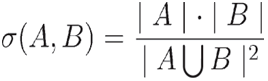
\includegraphics[scale=.33]{images/binary_diffing/similarity_function.png} \\
    \end{center}
    \begin{itemize}
        \item By maintaining large trees of malware, new and unidentified malware can  be immediately assigned into a family for classification and porting
    \end{itemize}
\end{frame}

\begin{frame}
    \frametitle{Phylogenetic Classification}
    \begin{itemize}
        \item Using the previously defined equation, distance matrices can be generated:
    \end{itemize}
    \begin{center}
    \begin{tiny}
    \begin{tabular}{l|rrrrrr}
                 & mimail.a & mimail.b & mimail.c & mimail.d & mimail.e & mimail.f \\ \hline
        mimail.a & 0        & 90.8     & 85.4     & 87.4     & 75.0     & 75.0     \\
        mimail.b & 90.8     & 0        & 84.7     & 88.0     & 74.3     & 74.3     \\
        mimail.c & 85.4     & 84.7     & 0        & 81.5     & 81.3     & 81.3     \\
        mimail.d & 87.4     & 88.0     & 81.5     & 0        & 72.3     & 72.3     \\
        mimail.e & 75.0     & 74.3     & 81.3     & 72.3     & 0        & 95.4     \\
        mimail.f & 75.0     & 74.3     & 81.3     & 72.3     & 95.4     & 0        \\
    \end{tabular}
    \end{tiny}
    \end{center}
\end{frame}

\begin{frame}
    \frametitle{Phylogenetic Classification}
    \begin{itemize}
        \item X-tree clustering algorithm can be applied to distance matrices
    \end{itemize}
    \begin{center}
        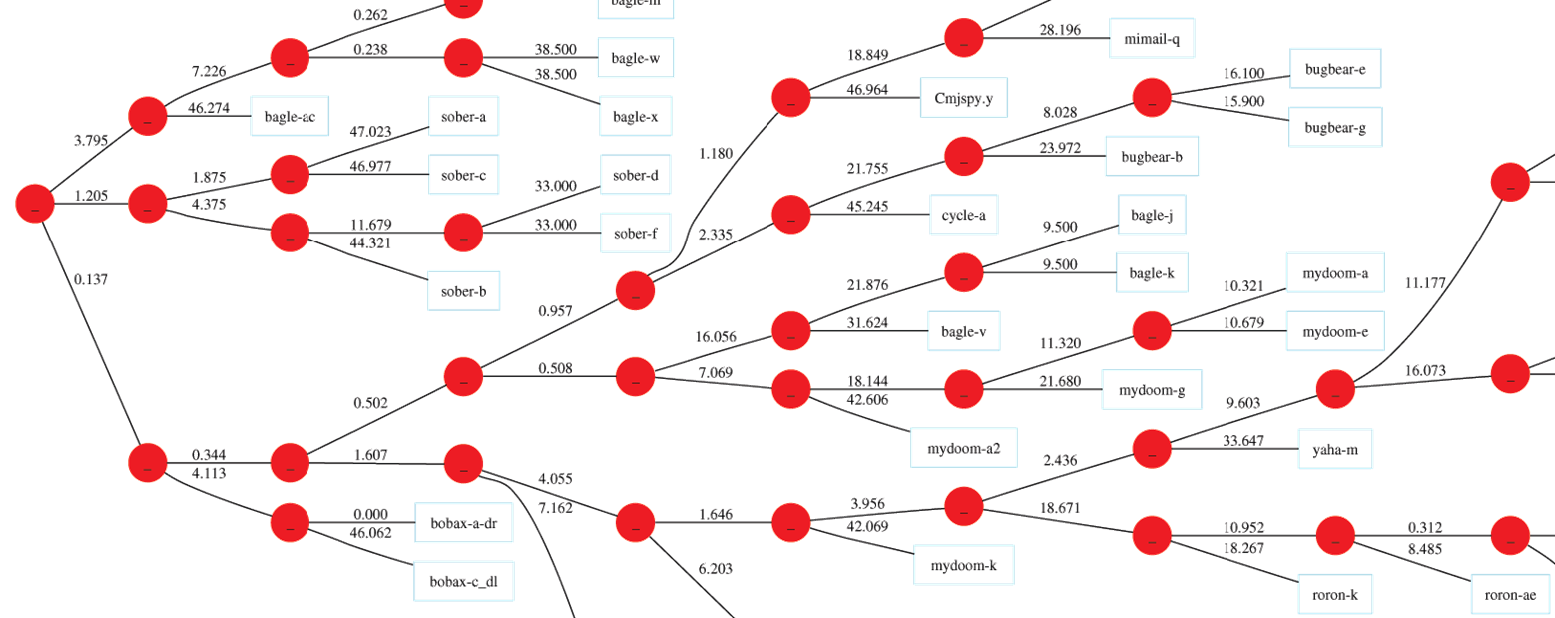
\includegraphics[scale=.50]{images/binary_diffing/xtree.png} \\
    \end{center}
\end{frame}


\subsection{Exercises}
\begin{frame}
    \frametitle{Exercise}
    \begin{itemize}
        \item Port work from Mydoom.D to Mydoom.M
        \item Any notable changes?
        \item Examine the differences between the dropped backdoors
    \end{itemize}
\end{frame}

\section{Advanced Malware Techniques}
\subsection{Advanced Malware Techniques}


\subsection{Anti-Detection/Obfuscation Measures}

\begin{frame}
    \frametitle{Detection Techniques and Counter-Measures}
    \begin{block}{}
        In order to detect malicious malware samples most of the antivirus industry relies on signature matching for detecting malware
    \end{block}
    \begin{itemize}
        \item A set of techniques will aim at making the signature based matching useless against identifying malware: polymorphism, server side polymorphism, metamorphism
        \item Others just aim at making analysis difficult or painful: code obfuscation, virtual machines, entry point obfuscation
    \end{itemize}
\end{frame}



\begin{frame}
    \frametitle{Polymorphism}
    \begin{itemize}
        \item Polymorphic malware generates different binaries as it spreads
        \item Performs relatively simple instruction substitutions or scrambling
        \item Changes key/algorithm in every iteration
        \item Code keeps some similar patterns across generations
        \item Not truly problematic, live analysis is usually an effective measure. High-level behavior seldom changes
    \end{itemize}
\end{frame}

\begin{frame}
    \frametitle{A View of Polymorphism}
    \begin{center}
        \pgfimage[height=7cm]{images/advanced_malware_techniques/polymorphic}
    \end{center}
\end{frame}


\begin{frame}
    \frametitle{Metamorphism}
    \begin{itemize}
        \item Metamorphic malware doesn't just scramble the code but actually generates new code
        \item Disassembles and reassembles itself, performing the same actions using different code
        \item Goes beyond simple instruction substitution
        \item Signature based detection has a tough time
    \end{itemize}
\end{frame}

\begin{frame}
    \frametitle{A View of Metamorphism}
    \begin{center}
        \pgfimage[height=7cm]{images/advanced_malware_techniques/metamorphic}
    \end{center}
\end{frame}


\begin{frame}
    \frametitle{Examples of Metamorphism}
    \begin{block}<1->{}
        \pedref{PFerrie-zmist}
    \end{block}
    \begin{block}<1->{}
        \pedref{evol}
    \end{block}
    \begin{block}<1->{}
        \pedref{PEferrie-simile} (Metamorphic Permutating High-Obfuscating Reassembler)
    \end{block}
\end{frame}


\begin{frame}
    \frametitle{Entry Point Obfuscation}
    \begin{itemize}
        \item Used by file infectors
        \item Hides the entry point to the malicious code
        \item Finds some functionality of the host application that it's always executed
        \item Then it diverts the execution flow to its own code, eventually returning to the original code
        \item The Polip family is a good example
        \begin{block}{}
            \begin{center}
                Try writing a small IDAPython script to automatically find the entrypoints to the malicious code
            \end{center}
        \end{block}        
    \end{itemize}
\end{frame}


\begin{frame}
    \frametitle{Virtual Machines}
    \begin{itemize}
        \item Aims at making analysis difficult 
        \item Removes the logic of the code by implementing a virtual architecture on which the final code is developed
        \item An analyst must first unfold this machine's architecture in order to understand the higher level code
    \end{itemize}
\end{frame}

\begin{frame}
    \frametitle{Examples of Virtual Machine Technology}
    \begin{itemize}
        \item Themida
            \begin{block}{}
                \begin{center}
                    http://www.oreans.com/themida.php
                \end{center}
            \end{block}        
        \item VMProtect
            \begin{block}{Source Code}
                \begin{center}
                    http://www.polytech.ural.ru/ (in Russian)
                \end{center}
            \end{block}
        \item StarForce
            \begin{block}{}
                \begin{center}
                    http://www.star-force.com/
                \end{center}
            \end{block}        
        \item T2 Conference Challenge and a few other "crackmes"
    \end{itemize}
\end{frame}



\subsection{Runtime Hiding Techniques}

\begin{frame}
    \frametitle{Rootkit Technology}
    
    \begin{block}{Overview}
    Rootkits aim at making themselves and other executables undetectable to the underlying system. For malware, the main purpose of rootkit technology is to remain on the infected host as long as possible without being detected and therefore disinfected
    \end{block}
    \begin{itemize}
        \item Rootkits normally run in kernel mode
        \item Commonly they hook \emph{API} functionality and filter those events that would expose them
        \item \emph{DKOM} (\emph{Direct Kernel Object Manipulation}) is a more advanced technique by which rootkits alter executive objects in order to remove any traces of them running
    \end{itemize}
\end{frame}


\begin{frame}
    \frametitle{Hypervisor Technology}
    \begin{block}{\emph{From Wikipedia}}
        A hypervisor in computing is a scheme which allows multiple operating systems to run, unmodified, on a host computer at the same time. The term is an extension of the earlier term supervisor, which was commonly applied to operating system kernels in that era.
    \end{block}

\end{frame}

\begin{frame}
    \frametitle{Hypervisor Technology}
    
    \begin{itemize}
        \item Both \emph{Intel} and \emph{AMD} have their own hardware virtualization extensions
        \item \emph{AMD}'s is currenly codenamed \emph{Pacifica}
        \item \emph{Intel}'s is known as \emph{VT} or \emph{Vanderpool}
        \item Both technologies are already available on consumer products.
        \item \emph{Microsoft's} \emph{Virtual PC} and \emph{Virtual Server}, \emph{Parallels Workstation}, \emph{TRANGO}, \emph{VMware} and \emph{Xem} already employ the virtualization extensions if available
        \item \emph{Blue Pill} uses undocumented features in \emph{Pacifica} to take over the system
    \begin{block}{}
        \begin{center}
            http://theinvisiblethings.blogspot.com/2006/06/introducing-blue-pill.html
        \end{center}
    \end{block}
    \end{itemize}
\end{frame}


\subsection{Counter-Measures}
\begin{frame}
    \frametitle{Poly/Meta morphism}
    \begin{itemize}
        \item Polymorphism can be fought with emulation and live analysis techniques
        \item Metamorphism and VM techniques are trickier
        \item Behavioral analysis is effective as long as the malware in question performs distinctive actions using common APIs
    \end{itemize}
\end{frame}

\begin{frame}
    \frametitle{Rootkits}
    \begin{itemize}
        \item To detect active rootkits one of the common approaches is to attempt to gather the same information through different channels. For instance:        
        \begin{itemize}
            \item Using the operating system's standard \emph{API}s
            \item Using low level techniques, thus bypassing the \emph{API}s
            \item Attempting to obtain handles to every possible process
        \end{itemize}
        \item Proceeding to compare the two sets of results. Disparities between them will tend to indicate that something might trying to hide
        \item Detecting hardware-virtualized malware might actually be impossible if the implementation has no bugs... ;-)
    \end{itemize}
\end{frame}
% included by ../header.tex

\part{Analysis and Custom Development}

\section{Analysis}
\subsection{Analysis I}
\begin{frame}
    \frametitle{The Target}
    \pgfimage[width=5cm]{images/analysis_I/virus_I_mugshot}
    \begin{block}{}
        \begin{itemize}
            \item SHA1: \emph{c9f10fa5135e3f10c1fb942d12bb8f267e4203d0}
            \item MD5: \emph{04c94ee7122a2844e12afe0928806fa0}
        \end{itemize}
    \end{block}
\end{frame}

\begin{frame}
    \frametitle{Is it Packed?}
    \begin{itemize}
        \item<+-> If so, generally there are no visible strings.
            \pedbullet{<+->\alert{Remember: Unicode strings have a non-occidental charset}}
        \item<+-> Most common imports will not be present
        \item<+-> Perhaps only \texttt{LoadLibrary} and \texttt{GetProcAddress}
        \item<+-> Recall that we can utilize statistical tests as an indicator
            \pedbullet{<+->A high entropy indicates a \emph{very-likely-to-be-compressesed} data section}
    \end{itemize}
\end{frame}
        
\begin{frame}[t]
    \frametitle{What is it Packed With?}
  \begin{columns}[T]
    \begin{column}{6cm}
      \begin{itemize}
        \item Can we guess the packer?
        \item Does \emph{PEiD} help?
        \item Does a hexeditor expose any clues?
      \end{itemize}
    \end{column}
    \begin{column}{6cm}
        \pgfimage<1->[width=5.6cm]{images/analysis_I/UPX_hexdump_scrambled_strings}%
    \end{column}
  \end{columns}
\end{frame}

\begin{frame}[t]
    \frametitle{First Look in IDA}
    \begin{block}{}
        Notice that opening the file in \emph{IDA} results in complaints about a missing import table. The navigation bar reveals very little code. What we see is the \emph{UPX} unpacking code with its typical start and finish.
    \end{block}
  \begin{center}
    \pgfimage<1>[width=10cm]{images/analysis_I/UPX_unpacker_code_start}
    \pgfimage<2>[width=10cm]{images/analysis_I/UPX_unpacker_code_end}
  \end{center}
\end{frame}

\begin{frame}
    \frametitle{Bypassing UPX}
    \begin{itemize}
        \item<+-> Despite its simplicity, \emph{UPX} is very commonly used
        \item<+-> Set a breakpoint at the jump to the \emph{OEP} (\alert{not in the destination})
        \item<+-> Continue the process and let the unpacker do its work
        \item<+-> Once the breakpoint is hit we can step to the next instruction to find the unpacked code
    \end{itemize}
\end{frame}

\begin{frame}[t]
    \frametitle{OEP Before and After}
    \begin{center}
        \pgfimage<1>[height=6cm]{images/analysis_I/UPX_oep_not_unpacked}
        \pgfimage<2>[height=6cm]{images/analysis_I/UPX_oep_unpacked}
    \end{center}
\end{frame}

\begin{frame}
    \frametitle{Dumping the Image}
    \begin{itemize}
        \item<+-> We need to save the unpacked image to disk for analysis
        \item<+-> The \emph{OllyDump} plugin can do this for us
        \item<+-> \emph{OllyDump} can also rebuild the \emph{IAT}
        \item<+-> \emph{ProcDump} and \emph{ImpRec} are other tools for accomplishing the job
        \item<+-> Now we are ready to jump back to IDA
    \end{itemize}
\end{frame}

\begin{frame}
    \frametitle{The Analysis}
    \begin{block}{}
        This executable has a range of interesting features and there are certain considerations to take into account during the analysis
    \end{block}
    \pause
    \begin{itemize}
        \item<+-> A good amount of code is not properly recognized, we will need to manually define it
        \item<+-> Function ends are often not found properly, we must manually fix these
        \item<+-> There will be tables of pointers interleaved within the code, these are \emph{Delphi}'s structures
        \item<+-> \emph{IDA} might not recognize library functions, therefore we might need to spot these manually
        \item<+-> A good approach is to linearly scan the binary (if it's not too large)
    \end{itemize}
\end{frame}

\begin{frame}[fragile]
    \frametitle{Exploring the Binary}
    One of the first functions, called (at \emph{40F37Bh}) is interesting.\\
    We can get to it in two ways. One is exploring from the beginning of the binary and the second is by following backwards references like the following
        \begin{block}{}
            \begin{semiverbatim}
\uncover{.UPX0:0040AC62 11AC        mov     eax, ds:off_412828}
\uncover{.UPX0:0040AC67 11AC        mov     eax, [eax]}
\uncover{.UPX0:0040AC69 11AC        call    eax}
            \end{semiverbatim}
        \end{block}
\end{frame}

\begin{frame}[fragile]
    \frametitle{Exploring the Binary}
        \begin{block}{}
            \begin{semiverbatim}
\uncover{.UPX0:0040AC62 11AC        mov     eax, ds:off_412828}
\uncover{.UPX0:0040AC67 11AC        mov     eax, [eax]}
\uncover{.UPX0:0040AC69 11AC        call    eax}
            \end{semiverbatim}
        \end{block}

        \begin{itemize}
            \item<2->{Following the offset \emph{off\_412828} we will find ourselves at \emph{413D44h}. This address has two references and is actually written to by one of them (\emph{DATA XREF: sub\_406764+288})\\}
            \item<3->{Inspecting the reference we see this and other addresses are being written to, all of which are called\\}
            \item<4->{Hence we have more imports to fix. This time the program seems to be using a hash based approach, where it's difficult to tell the import from the value fed}
        \end{itemize}
\end{frame}

\begin{frame}[fragile]
    \frametitle{Resolving the Imports}
    If we trace the function with \emph{OllyDbg} we can see that a good set of \emph{API} functions are imported
        \begin{block}{}
        \small
            \begin{semiverbatim}
.UPX0:004069E0 030         mov     [ebx], eax
.UPX0:004069E2 030         mov     eax, 0A7733ACDh
.UPX0:004069E7 030         call    resolve_import
.UPX0:004069E7
.UPX0:004069EC 030         mov     ds:send, eax
.UPX0:004069F1 030         mov     eax, 0A0F5FC93h
.UPX0:004069F6 030         call    resolve_import
.UPX0:004069F6
.UPX0:004069FB 030         mov     ds:WSAStartUp, eax
.UPX0:00406A00 030         mov     eax, 5E568BBh
.UPX0:00406A05 030         call    resolve_import
.UPX0:00406A05
.UPX0:00406A0A 030         mov     ds:socket, eax
            \end{semiverbatim}
        \end{block}
\end{frame}

\begin{frame}
    \frametitle{A Quick Glimpse of the Imports}
    \begin{itemize}
        \item Of special interest are the functions from the networking \emph{API}
        \item Combined with a look at the imports gives us dire forecast
        \item Further inspection reveals that this is indeed malicious
    \end{itemize}
  \begin{center}
    \pgfimage[height=3cm]{images/analysis_I/IDA_urldownloadtofile}
    \pgfimage[height=3cm]{images/analysis_I/IDA_winexec}
  \end{center}    
\end{frame}

\begin{frame}[fragile]
    \frametitle{Interesting Code Construct}
        \begin{block}{}
            \small
            \begin{semiverbatim}
.UPX0:00406086 000         mov     eax, eax
.UPX0:00406088 000         push    ebx
.UPX0:00406089 004         push    esi
.UPX0:0040608A 008         mov     esi, edx
.UPX0:0040608C 008         mov     ebx, eax
.UPX0:0040608E 008         push    esi
.UPX0:0040608F 00C         push    ebx
.UPX0:00406090 010         call    ds:__WSAFDIsSet
.UPX0:00406090
.UPX0:00406096 008         cmp     eax, 1
.UPX0:00406099 008         sbb     eax, eax
.UPX0:0040609B 008         inc     eax
.UPX0:0040609C 008         pop     esi
.UPX0:0040609D 004         pop     ebx
.UPX0:0040609E 000         retn
            \end{semiverbatim}
        \end{block}
\end{frame}

\begin{frame}[fragile]
    \frametitle{Branchless Logic}
        \begin{block}{}
            \begin{semiverbatim}
                cmp     eax, 1
                sbb     eax, eax
                inc     eax
                pop     esi
                pop     ebx
                retn
            \end{semiverbatim}
        \end{block}
        \begin{itemize}
            \item<1-> \alert{cmp eax, 1} will set the carry flag (\alert{CF}) if \alert{eax} is 0
            \item<2-> \alert{sbb eax, eax} does \alert{eax = eax - (eax+CF)}
            \item<3-> Therefore if \alert{eax} was 0 we have \alert{eax = 0 - (0+1) = -1}
            \item<4-> Otherwise if \alert{eax} is greater than 0 we have \alert{eax = eax - eax+0 = 0}
            \item<5-> The increment will set the possible \alert{eax} values to 1 or 0
        \end{itemize}
\end{frame}

\begin{frame}
    \frametitle{Hotspots}
    Points of interest in the binary are
    \begin{itemize}
        \item Import resolution \emph{40F37Bh}
        \item Deobfuscation function \emph{406464h}
        \item \emph{NetBios} spreading \emph{409408h}
        \item Connect to \emph{Mydoom}'s backdoor \emph{409E50}
        \item Download and execute \emph{40AE30h}
        \item Build system info summary \emph{40BA14h}
        \item Handle \emph{IRC} commands \emph{40C330h}
    \end{itemize}
\end{frame}

\begin{frame}
    \frametitle{The Target Revealed}
  \begin{columns}[c]
    \begin{column}{5.2cm}
        \pgfimage[width=5cm]{images/analysis_I/virus_I_mugshot}
    \end{column}
    \begin{column}{6.5cm}
        \begin{block}{}
            \begin{itemize}
                \item Kaskpersky: \emph{Backdoor.Win32.Gobot.w}
                \item McAfee: \emph{Exploit-Mydoom}
                \item Symantec: \emph{W32.Gobot.A} 
                \item Trend Micro: \emph{BKDR\_GOBOT.W}
            \end{itemize}
        \end{block}
    \end{column}
  \end{columns}

    \begin{block}{}
        \begin{itemize}
            \item SHA1: \emph{c9f10fa5135e3f10c1fb942d12bb8f267e4203d0}
            \item MD5: \emph{04c94ee7122a2844e12afe0928806fa0}
        \end{itemize}
    \end{block}
\end{frame}


\subsection{Analysis II}
\begin{frame}
    \frametitle{The Target}
    \pgfimage[width=5cm]{images/analysis_II/virus_II_mugshot}
    \begin{block}{}
        \begin{itemize}
            \item SHA1: \emph{f30ad924a0d35b13d2057b1bb6305ad5a8ac8fa2}
            \item MD5: \emph{0af7b122bb722fb679c97fdb8cf85d23}
        \end{itemize}
    \end{block}
\end{frame}

\begin{frame}
    \frametitle{Is it Packed?}
    \begin{itemize}
        \item<+-> If so, generally there are no visible strings.
            \pedbullet{<+->\alert{Remember: Unicode strings have a non-occidental charset}}
        \item<+-> Most common imports will not be present
        \item<+-> Perhaps only \texttt{LoadLibrary} and \texttt{GetProcAddress}
        \item<+-> Recall that we can utilize statistical tests as an indicator
            \pedbullet{<+->A high entropy indicates a \emph{very-likely-to-be-compressesed} data section}
    \end{itemize}
\end{frame}
        
\begin{frame}[t]
    \frametitle{What is it Packed With?}
  \begin{columns}[T]
    \begin{column}{6cm}
      \begin{itemize}
        \item Can we guess the packer?
        \item Does \emph{PEiD} help?
        \item Does a hexeditor expose any clues?
      \end{itemize}
    \end{column}
    \begin{column}{6cm}
        \pgfimage<2->[width=5.6cm]{images/analysis_II/UPX_hexdump_scrambled_strings}%
    \end{column}
  \end{columns}
\end{frame}

\begin{frame}
    \frametitle{First look in IDA (1)}
    Here we can see a basic obfuscation technique. Upon execution it will first go through an \emph{XOR} loop to reveal some additional code. Execution continues at the unveiled code
  \begin{center}
    \pgfimage[width=10cm]{images/analysis_II/IDA_1st_xor_loop}
  \end{center}
\end{frame}

\begin{frame}
    \frametitle{First look in IDA (2)}
    This is the result after the deobfuscation is finished
  \begin{center}
    \pgfimage[width=8cm]{images/analysis_II/IDA_1st_xor_loop_after}
  \end{center}
\end{frame}

\begin{frame}
    \frametitle{Lack of imports}
    We can now follow the newly available code in \emph{IDA}.
    We soon realize that there's not much we can tell as there are no imported symbols available
  \begin{center}
    \pgfimage[width=8cm]{images/analysis_II/IDA_parite_code_no_imports}
  \end{center}
\end{frame}

\begin{frame}[t]
    \frametitle{\emph{OllyDbg} to the Rescue}
    \emph{OllyDbg} can help in this case.
    \begin{itemize}
        \item<2-> Tracing to the interesting locations, we can see where the addresses are actually pointing to
        \item<3-> The binary is resolving the imported symbols by itself
    \end{itemize}
  \begin{center}
    \pgfimage<2-2>[width=11cm]{images/analysis_II/OllyDBG_00_calling_loadlibrary}
    \pgfimage<3-3>[width=10cm]{images/analysis_II/OllyDBG_01_resolving_imports}
    \pgfimage<4->[width=8cm]{images/analysis_II/OllyDBG_02_resolved_imports_in_the_stack}
  \end{center}
\end{frame}

\begin{frame}[fragile]
    \frametitle{Resolving Imports}
    \begin{itemize}
        \item Two functions are used \emph{LoadLibrary} and \emph{GetProcAddress}
    \end{itemize}
    \begin{block}{}
    \begin{semiverbatim}
HMODULE WINAPI LoadLibrary
(
    LPCTSTR lpFileName
);

FARPROC WINAPI GetProcAddress
(
    HMODULE hModule, LPCSTR lpProcName
);
    \end{semiverbatim}
    \end{block}
\end{frame}

\begin{frame}
    \frametitle{Imports fixed...}
    \begin{itemize}
        \item The imported symbols appear mainly to relate to file access operations
        \item We can track the flow further in \emph{OllyDbg} and conveniently comment the \emph{API} call names in \emph{IDA} for later reference
        \item We can also locate the table of addresses and write a small script to do it for us. More on that later
        \item After some tracing it is possible to see that the file being executed is opened, seeked and then its contents written to disk after yet another \emph{XOR}'ing loop
    \end{itemize}
\end{frame}

\begin{frame}
    \frametitle{Main Deobfuscation Function}
  \begin{center}
    \pgfimage[height=6cm]{images/analysis_II/IDA_parite_body_xor_function}
  \end{center}
\end{frame}

\begin{frame}
    \frametitle{Now What?}
    \begin{itemize}
        \item After the file is entirely dumped to disk, it is loaded as a \emph{DLL} (Typical \emph{LoadLibrary}, \emph{GetProcAddress}, \emph{call} sequence)
        \item If we take a look at the dumped file we can see that, yet again, it's packed. But this time it is a \emph{DLL}
        \item The unpacking code is in the \emph{DLLEntryPoint} (automatically called when doing invoking \emph{LoadLibrary})
        \item The main sample will resolve the \emph{Initiate} procedure and call it
    \end{itemize}
\end{frame}

\begin{frame}
    \frametitle{Dumping a DLL}
    \begin{itemize}
        \item<+-> If we want the unpacked contents of the binary we can use \emph{ProcDump} to dump the \emph{DLL} from memory
        \item<+-> Now we have the code but not the imports
            \pedbullet{And fixing the imports for a \emph{DLL} is not trivial}
    \end{itemize}
  \begin{center}
    \pgfimage[width=8cm]{images/analysis_II/ProcDump_dumping_the_dropped_and_loaded_dell}
  \end{center}
\end{frame}

\begin{frame}
    \frametitle{Fixing Imports}
    \begin{itemize}
        \item<+-> If we followed all along with \emph{OllyDbg}, it is possible to find the imported \emph{API} calls becase \emph{UPX} did the work of resolving them for us when the \emph{DLL} was loaded
        \item<+-> We will track the execution to find the table of imported symbols
        \item<+-> We will then extract that info and use it in \emph{IDA}
    \end{itemize}
\end{frame}

\begin{frame}
    \frametitle{Fixing Imports (1)}
    The execution is followed until the dropped \emph{DLL} is loaded and its \emph{Initiate} exported function called
  \begin{center}
    \pgfimage[width=10cm]{images/analysis_II/OllyDBG_03_calling_the_dlls_Initiate}
  \end{center}
\end{frame}

\begin{frame}
    \frametitle{Fixing Imports (2)}
    \begin{itemize}
        \item We step into and try to find an instance where a call to an imported symbol is made
        \item \emph{OllyDbg} will indicate this by displaying a \emph{DLL.Function} name on the right side of the disassembly
    \end{itemize}
  \begin{center}
    \pgfimage[width=11cm]{images/analysis_II/OllyDBG_04_calling_a_dll_resolved_import}
  \end{center}
\end{frame}

\begin{frame}
    \frametitle{Fixing Imports (3)}
    Following the jump we find what we wanted. The table with all the symbols!
  \begin{center}
    \pgfimage[width=10cm]{images/analysis_II/OllyDBG_05_the_dlls_table_of_imported_symbols}
  \end{center}
\end{frame}

\begin{frame}
    \frametitle{Being Inventive (1)}
    \begin{itemize}
        \item<+-> Now that we have found all the imported symbols for the \emph{DLL}, we want to be able to port it over to our disassembly
        \item<+-> One possible approach is to use \emph{IDAPython} and some C\&P'ing
    \end{itemize}
\end{frame}
    
\begin{frame}
    \frametitle{Being Inventive (2)}
    \begin{itemize}
        \item<+-> Lets copy the entire list from \emph{OllyDbg} and paste it in a decent editor with regex substitution support
        \item<+-> Now some regex magic...
            \begin{block}{}
                \begin{center}
                    ([0-9ABCDEF]+).*jmp.*; (.*) \\
                    MakeName($\backslash$1, '$\backslash$2')
                \end{center}
            \end{block}
    \end{itemize}
\end{frame}

\begin{frame}
    \frametitle{Being Inventive (3)}
    \begin{itemize}
        \item<+-> ...and turn it into something sexier
            \begin{block}{}
                MakeName(0x008E2DA0, 'advapi32.RegCloseKey')\\
                MakeName(0x008E2DA6, 'advapi32.RegCreateKeyExA')\\
                MakeName(0x008E2DAC, 'advapi32.RegFlushKey')\\
                MakeName(0x008E2DB2, 'advapi32.RegOpenKeyExA')\\
                ...
            \end{block}
        \item<+-> Copy the converted text into \emph{IDAPython}'s notepad and execute it
        \item<+-> Now, we will have all the names in our dumped \emph{DLL}
    \end{itemize}
\end{frame}


\begin{frame}
    \frametitle{Main Deobfuscation Function}
  \begin{center}
    \pgfimage[height=6cm]{images/analysis_II/IDA_parite_fixed_imports}
  \end{center}
\end{frame}

\begin{frame}
    \frametitle{Is That All?}
    \begin{itemize}
        \item<1-> You might think that the unpacking is now complete... unfortunately that's only partially true
        \item<2-> If we follow the flow further we will eventually find that it does not exit
        \item<3-> Instead we find ourselves in \emph{UPX} unpacking code...
        \item<4-> ... unpacking again?
    \end{itemize}
\end{frame}

\begin{frame}
    \frametitle{The Follow Up}
    \begin{itemize}
        \item \emph{UPX} is pretty simple to deal with
        \item We just move to the end of the unpacking code and look at the jump
        \item It's indeed \emph{UPX} and after the unpacking is done execution will continue within the binary
        \item If we breakboint the jump and let it unpack we can dump the new executable
    \end{itemize}
  \begin{center}
    \pgfimage[height=3.7cm]{images/analysis_II/IDA_UPX_jump_to_oep}
  \end{center}
\end{frame}

\begin{frame}
    \frametitle{The 2nd Unpacked Component}
    After some inspection it's possible to find that this new element is certainly malicious (as is the \emph{DLL})
  \begin{center}
    \pgfimage[height=3cm]{images/analysis_II/IDA_urldownloadtofile}
    \pgfimage[height=3cm]{images/analysis_II/IDA_winexec}
  \end{center}    
\end{frame}

\begin{frame}
    \frametitle{Final Outcome}
    \begin{itemize}
        \item \alert{What's the explanation?}
        \item The second sample is a Bot, specifically \emph{Backdoor.Win32.Gobot.w} or \emph{W32.Gobot.A}, depending on who you ask
        \item The first sample was \emph{Parite}
        \item \emph{Parite} is a polymorphic file infector and we just saw it in action
    \end{itemize}
\end{frame}

\begin{frame}
    \frametitle{The Target Revealed}
  \begin{columns}[c]
    \begin{column}{5.2cm}
        \pgfimage[width=5cm]{images/analysis_II/virus_II_mugshot}
    \end{column}
    \begin{column}{6.5cm}
        \begin{block}{}
            \begin{itemize}
                \item Kaskpersky: \emph{Virus.Win32.Parite.b}
                \item McAfee: \emph{W32/Pate.b}
                \item Symantec: \emph{W32.Pinfi} 
                \item Trend Micro: \emph{PE\_PARITE.A}
            \end{itemize}
        \end{block}
    \end{column}
  \end{columns}
    \begin{block}{}
        \begin{itemize}
            \item SHA1: \emph{f30ad924a0d35b13d2057b1bb6305ad5a8ac8fa2}
            \item MD5: \emph{0af7b122bb722fb679c97fdb8cf85d23}
        \end{itemize}
    \end{block}
\end{frame}


\section{IDA Python}
\subsection{Overview}
\begin{frame}
    \frametitle{What is it?}
    \begin{itemize}
        \item IDAPython extends IDA with Python
        \item The whole IDC function set and the plugin API are available
        \item Python is an incredibly powerful scripting language
        \item The blend allows for extreme flexibility when writing custom analysis tools
        \item \emph{ida2sql}, for instance, was written using IDAPython and exports nearly the whole IDB to an SQL database for advanced and automated data-mining
    \end{itemize}
\end{frame}

\begin{frame}
    \frametitle{Resources}
    \begin{itemize}
        \item First introduced in the paper "Digital Genome Mapping - Advanced Binary Malware Analysis"
        \begin{block}{}
            \pedref{CarreraErdelyiVB04}
        \end{block}{}
        \item Available for download from:
        \begin{block}{}
            \begin{center}
                http://d-dome.net/idapython
            \end{center}
        \end{block}{}
        \item Good article on OpenRCE: "Introduction to IDAPython"
        \begin{block}{}
            \pedref{IDAPythonIntro}
        \end{block}
        \item ida2sql is available at:
        \begin{block}{}
            \begin{center}
                http://dkbza.org/ida2sql.html
            \end{center}
        \end{block}{}
    \end{itemize}
\end{frame}


\subsection{Examples}
\begin{frame}[fragile]
    \frametitle{Reading a string}
Reading and printing a string from the current cursor location:
    \begin{block}{}
        \begin{semiverbatim}
\uncover{ea = ScreenEA()}
\uncover{}
\uncover{s = ""}
\uncover{while True:}
\uncover{   b = Byte(ea)}
\uncover{   if b == 0:}
\uncover{       break}
\uncover{   s += chr(b)}
\uncover{   ea += 1}
\uncover{}
\uncover{print s}
        \end{semiverbatim}
    \end{block}
\end{frame}

\begin{frame}[fragile]
    \frametitle{XOR-ing a string}
    \begin{block}<1->{}
        \begin{semiverbatim}
\uncover{ea = ScreenEA()}
\uncover{}
\uncover{s = ""}
\uncover{while True:}
\uncover{   b = Byte(ea)}
\uncover{   if b == 0:}
\uncover{       break}
\uncover{   b = b^0xff}
\uncover{   PatchByte(ea, b)}
\uncover{   ea += 1}
\uncover{}
\uncover{print s}
        \end{semiverbatim}
    \end{block}
\end{frame}

\begin{frame}[fragile]
    \frametitle{Enumerating Segments}
    \begin{block}<1->{}
        \begin{semiverbatim}
\uncover{for seg in Segments():}
\uncover{   print '%08x-%08x' % (seg, SegEnd(seg))}
        \end{semiverbatim}
    \end{block}
\end{frame}

\begin{frame}[fragile]
    \frametitle{Enumerating Functions}
    \begin{block}<1->{}
        \begin{semiverbatim}
\uncover{for f in Functions(start\_addr, end\_addr):}
\uncover{   print '%s: %08x-%08x' % (Name(f), f, FindFuncEnd(f))}
        \end{semiverbatim}
    \end{block}
\end{frame}

\begin{frame}[fragile]
    \frametitle{Enumerating Heads}
    \begin{block}<1->{}
        \begin{semiverbatim}
\uncover{for h in Heads(ScreenEA(), ScreenEA()+100):}
\uncover{   print hex(h)}
        \end{semiverbatim}
    \end{block}
\end{frame}


\begin{frame}
    \frametitle{Collecting Function Chunks}
    \begin{itemize}
        \item     Some compilers generate optimized code containing features such as
            \pedbullet{Functions share basic blocks}
            \pedbullet{The layout of \emph{basic blocks} within the binary is affected by the likelihood of them being run}
        \item \emph{IDA} handles the resulting "fragmented" functions by collecting all the parts in chunks
        \item The functions \emph{func\_tail\_iterator\_t()}, \emph{func\_iter.main()}, \emph{func\_iter.chunk()}, \emph{func\_iter.next()} allow to retrieve them
    \end{itemize}
\end{frame}


\begin{frame}[fragile]
    \frametitle{Collecting Function Chunks (2)}
    \begin{block}<1->{}
    \begin{small}
        \begin{semiverbatim}
\uncover{ function_chunks = []}
\uncover{ #Get the tail iterator}
\uncover{ func_iter = idaapi.func_tail_iterator_t(idaapi.get_func(ea))}
\uncover{}
\uncover{ # While the iterator's status is valid}
\uncover{ status = func_iter.main()}
\uncover{ while status:}
\uncover{  # Get the chunk}
\uncover{  chunk = func_iter.chunk()}
\uncover{  # Store its start and ending address as a tuple}
\uncover{  function_chunks.append((chunk.startEA, chunk.endEA))}
\uncover{  # Get the last status}
\uncover{  status = func_iter.next()}
        \end{semiverbatim}
    \end{small}
    \end{block}
\end{frame}


\subsection{Exercises}
\begin{frame}
    \frametitle{Mydoom Backdoor DLL Extraction}
    \begin{itemize}
        \item Locate the DLL bytes in memory
        \item Locate the DLL decoder
        \item Write an IDA Python script to decode and save the DLL to disk
    \end{itemize}
\end{frame}

\begin{frame}
    \frametitle{Mydoom String De-obfuscation}
    \begin{itemize}
        \item Locate some obfuscated strings
        \item Determine the obfuscation method
        \item Write an IDA Python script to restore the original strings
    \end{itemize}
\end{frame}

\section{PEFile and PyDasm}
\subsection{Overview}
\begin{frame}
    \frametitle{Purpose}
    \begin{itemize}
        \item Python libraries that allow for scripted Windows binary inspection
        \item These tools allow for great automation of various analysis tasks
        \item \emph{pefile} is a PE Format Python parsing module
        \item \emph{pydasm} is an \emph{x86} Python disassembler module
            \pedbullet{pydasm is used by PaiMei (we may talk about this later)}
    \end{itemize}
\end{frame}

\begin{frame}
    \frametitle{pefile}
    \begin{block}{}
        \begin{center}
            http://dkbza.org/pefile.html
        \end{center}
    \end{block}

    \begin{itemize}
        \item \emph{pefile} is a cross-platform pure Python module intended for handling PE Files
        \item Actively maintained by Ero
        \item It should be able to process any file that can be open by the Windows loader
        \item Usage requires some basic understanding of the layout of a PE file
        \item You can use \emph{pefile} to explore nearly every single feature of a PE file
    \end{itemize}
\end{frame}


\subsection{pefile}
\begin{frame}
    \frametitle{Loading a PE file}
    \begin{itemize}
        \item Loading a file is as easy as creating an instance of the PE class with a path to the PE file
            \begin{block}{}
                \begin{center}
                    pe = pefile.PE('path/to/file')
                \end{center}
            \end{block}
        \item Alternatively, you can pass a PE file as raw data
            \begin{block}{}
                \begin{center}
                    pe = pefile.PE(data=python\_string)
                \end{center}
            \end{block}
    \end{itemize}
\end{frame}

\begin{frame}[fragile]
    \frametitle{Inspecting the Headers}
    \begin{block}<1->{}
        \small
        \begin{semiverbatim}
\uncover{>>> import pefile}
\uncover{}
\uncover{>>> pe = pefile.PE('notepad.exe')}
\uncover{>>> hex(pe.OPTIONAL\_HEADER.ImageBase)}
\uncover{['0x1000000L']}
\uncover{}
\uncover{>>> hex(pe.OPTIONAL\_HEADER.AddressOfEntryPoint)}
\uncover{['0x6AE0L']}
\uncover{}
\uncover{>>> hex(pe.OPTIONAL\_HEADER.NumberOfRvaAndSizes)}
\uncover{['0x10L']}
\uncover{}
\uncover{>>> hex(pe.FILE\_HEADER.NumberOfSections)}
\uncover{['0x3']}
        \end{semiverbatim}
    \end{block}
\end{frame}

\begin{frame}[fragile]
    \frametitle{Inspecting the Sections}
    \begin{block}{}
        \begin{semiverbatim}
\uncover{>>> for section in pe.sections:}
\uncover{...  print (section.Name,}
\uncover{       hex(section.VirtualAddress),}
\uncover{       hex(section.Misc_VirtualSize),}
\uncover{       section.SizeOfRawData )}
\uncover{... }
\uncover{('.text', '0x1000L', '0x6D72L', 28160L)}
\uncover{('.data', '0x8000L', '0x1BA8L', 1536L)}
\uncover{('.rsrc', '0xA000L', '0x8948L', 35328L)}
        \end{semiverbatim}
    \end{block}
\end{frame}

\begin{frame}[fragile]
    \frametitle{Think it's Packed?}
    \begin{block}{}
        \begin{semiverbatim}
\uncover{import math}
\uncover{}
\uncover{def H(data):}
\uncover{   if not data:}
\uncover{       return 0}
\uncover{}
\uncover{   entropy = 0}
\uncover{   for x in range(256):}
\uncover{       p_x = float(data.count(chr(x)))/len(data)}
\uncover{       if p_x > 0:}
\uncover{           entropy += - p_x*math.log(p_x, 2)}
\uncover{}
\uncover{   return entropy}
        \end{semiverbatim}
    \end{block}
\end{frame}

\begin{frame}[fragile]
    \frametitle{Think it's Packed? (Unpacked)}
    \begin{block}{}
        \begin{semiverbatim}
\uncover{>>> for section in pe.sections:}
\uncover{...  print section.Name, H(section.data)}
\uncover{... }
\uncover{.text 6.28370964662}
\uncover{.data 1.39795676336}
\uncover{.rsrc 5.40687515641}
        \end{semiverbatim}
    \end{block}
\end{frame}

\begin{frame}[fragile]
    \frametitle{Think it's Packed? (ASPack)}
    \begin{block}{}
        \begin{semiverbatim}
\uncover{>>> pe2 = pefile.PE('notepad-aspack.exe')}
\uncover{>>> for section in pe2.sections:}
\uncover{...  print section.Name, H(section.data)}
\uncover{... }
\uncover{.text 7.98363149339}
\uncover{.data 4.68226874255}
\uncover{.rsrc 6.09026175185}
\uncover{.aspack 5.90609875421}
\uncover{.adata 0}
        \end{semiverbatim}
    \end{block}
\end{frame}

\begin{frame}[fragile]
    \frametitle{Think it's Packed? (UPX)}
    \begin{block}{}
        \begin{semiverbatim}
\uncover{>>> pe3 = pefile.PE('notepad-upx.exe')}
\uncover{>>> for section in pe3.sections:}
\uncover{...  print section.Name, H(section.data)}
\uncover{... }
\uncover{UPX0 0}
\uncover{UPX1 7.83028313969}
\uncover{.rsrc 5.59212256596}
        \end{semiverbatim}
    \end{block}
\end{frame}

\begin{frame}[fragile]
    \frametitle{Imports}
    \begin{block}{}
        \begin{semiverbatim}
\uncover{>>> for entry in pe.DIRECTORY_ENTRY_IMPORT:}
\uncover{...   print entry.dll}
\uncover{...   for imp in entry.imports:}
\uncover{...     print '\\t', hex(imp.address), imp.name}
\uncover{... }
\uncover{comdlg32.dll}
\uncover{        0x10012A0L PageSetupDlgW}
\uncover{        0x10012A4L FindTextW}
\uncover{        0x10012A8L PrintDlgExW}
\uncover{[snip]}
\uncover{SHELL32.dll}
\uncover{        0x1001154L DragFinish}
\uncover{        0x1001158L DragQueryFileW}
        \end{semiverbatim}
    \end{block}
\end{frame}


\subsection{pydasm}

\begin{frame}
    \frametitle{pydasm}
    \begin{block}<1->{}
        \begin{center}
            http://dkbza.org/pydasm.html
        \end{center}
    \end{block}
    \begin{itemize}
        \item \emph{pydasm} is a cross-platform Python module wrapping jt's libdasm
        \item Combined with \emph{pefile}, you get a good base for developing a mini-IDA wannabe
    \end{itemize}
\end{frame}


\begin{frame}[fragile]
    \frametitle{Disassembling}
    \begin{block}{}
        \begin{semiverbatim}
\uncover{>>> import pydasm}
\uncover{>>> i = pydasm.get_instruction('\\x90', pydasm.MODE_32)}
\uncover{>>> pydasm.get_instruction_string(}
\uncover{       i, pydasm.FORMAT_INTEL, 0)}
\uncover{}
\uncover{['nop ']}
\uncover{}
\uncover{>>> i = pydasm.get_instruction(}
\uncover{       '\\x8B\\x04\\xBD\\xE8\\x90\\x00\\x01', pydasm.MODE_32)}
\uncover{>>> pydasm.get_instruction_string(}
\uncover{       i, pydasm.FORMAT_INTEL, 0)}
\uncover{}
\uncover{['mov eax,[edi*4+0x10090e8]']}
        \end{semiverbatim}
    \end{block}
\end{frame}

\begin{frame}[fragile]
    \frametitle{The Instruction Object}
    \begin{block}{}
        \begin{semiverbatim}
\uncover{>>> pprint.pprint(dir(i))}
\uncover{['__doc__','__module__',}
\uncover{ 'dispbytes', 'extindex',}
\uncover{ 'flags', 'fpuindex',}
\uncover{ 'immbytes', 'length',}
\uncover{ 'mode','modrm',}
\uncover{ 'op1', 'op2', 'op3',}
\uncover{ 'opcode', 'ptr',}
\uncover{ 'sectionbytes', 'sib',}
\uncover{ 'type']}
        \end{semiverbatim}
    \end{block}
\end{frame}

\begin{frame}[fragile]
    \frametitle{The Operand Object}
    \begin{block}{}
        \begin{semiverbatim}
\uncover{>>> pprint.pprint(dir(i.op1))}
\uncover{['__doc__', '__module__',}
\uncover{ 'basereg', 'dispbytes',}
\uncover{ 'displacement', 'dispoffset',}
\uncover{ 'flags', 'immbytes',}
\uncover{ 'immediate', 'immoffset',}
\uncover{ 'indexreg', 'reg',}
\uncover{ 'scale', 'section',}
\uncover{ 'sectionbytes', 'type']}
        \end{semiverbatim}
    \end{block}
\end{frame}

\begin{frame}[fragile]
    \frametitle{pefile+pydasm}
    \begin{block}{}
        \begin{semiverbatim}
\uncover{>>> ep = pe.OPTIONAL_HEADER.AddressOfEntryPoint}
\uncover{>>> ep_ava = ep+pe.OPTIONAL_HEADER.ImageBase}
\uncover{>>> data = pe.get_memory_mapped_image()[ep:ep+100]}
\uncover{>>> offset = 0}
\uncover{>>> while offset < len(data):}
\uncover{...   i = pydasm.get_instruction(}
\uncover{           data[offset:], pydasm.MODE_32)}
\uncover{...   print pydasm.get_instruction_string(}
\uncover{           i, pydasm.FORMAT_INTEL, ep_ava+offset)}
\uncover{...   offset += i.length}
        \end{semiverbatim}
    \end{block}
\end{frame}

\begin{frame}[fragile]
    \frametitle{pefile+pydasm (Output)}
    \begin{block}{}
    \small
        \begin{semiverbatim}
\uncover{push byte 0x70}
\uncover{push dword 0x1001888}
\uncover{call 0x1006ca8}
\uncover{xor ebx,ebx}
\uncover{push ebx}
\uncover{mov edi,[0x100114c]}
\uncover{call edi}
\uncover{cmp word [eax],0x5a4d}
\uncover{jnz 0x1006b1d}
\uncover{mov ecx,[eax+0x3c]}
\uncover{add ecx,eax}
\uncover{cmp dword [ecx],0x4550}
\uncover{jnz 0x1006b1d}
\uncover{movzx eax,[ecx+0x18}
        \end{semiverbatim}
    \end{block}
\end{frame}


\subsection{Exercises}
\begin{frame}
    \frametitle{pefile Exercises}
    \begin{itemize}
        \item Load a \emph{DLL} and print the imported and exported symbols
        \item Load a \emph{PE} file and check whether the entry point is in the last section and whether such section is smaller than the others
        \item Load a \emph{PE} file and dump the first 256 bytes, starting from the entry point, to disk
            \pedbullet{Think of a way of using this metadata as a packer or executable signature}
    \end{itemize}
\end{frame}

\begin{frame}
    \frametitle{pydasm Exercises}
    \begin{itemize}
        \item Building on the examples in the slides, create a disassembler that follows references and try to disassemble as far as you can
        \item Create a histogram from the mnemonics of the disassembled code
        \item Think of ways to use the histogram (or more advanced statistical techniques) to build a classifier based on entry point code
    \end{itemize}
\end{frame}


\section{PaiMei}
\subsection{Overview}
\begin{frame}
    \frametitle{The Man}
    \begin{center}
        
\includegraphics[scale=.5]{images/paimei/pstalker_demo.jpg} \\
    \end{center}
\end{frame}

\begin{frame}[t]
    \frametitle{What is it?}
    \begin{itemize}
        \item It's a win32 reverse engineering framework
        \item Written entirely in Python
        \item Think of PaiMei as an RE swiss army knife
        \item Already proven effective for a number of tasks
            \pedbullet{Fuzzer assistance}
            \pedbullet{Code coverage tracking}
            \pedbullet{Data flow tracking}
            \pedbullet{A beta tester used it to solve the T2'06 RE challenge}
    \end{itemize}
    \begin{block}{My hopes and dreams}
    That with community support and contributions, PaiMei can do for RE dev what Metasploit does for exploit dev
    \end{block}
\end{frame}

\begin{frame}[t]
    \frametitle{Motivation: Rapid Development}
    \begin{itemize}
        \item Avoid the learning / re-learning curve of various SDKs
        \item Develop in a higher level language
            \pedbullet{Easy management of arbitrary data structures}
            \pedbullet{Less code}
            \pedbullet{Less debugging of the actual tool}
        \item Build data representation \alert{into} the framework, as opposed to an after-thought
            \pedbullet{Of course, coming from Pedram, this translates into graphing}
    \end{itemize}
\end{frame}

\begin{frame}[t]
    \frametitle{Motivation: Homogenous Environment}
    \begin{itemize}
        \item Making tools and languages talk to one another is tedious
            \pedbullet{IDA vs. OllyDbg vs. MySQL}
            \pedbullet{C/C++ vs. Python}
        \item Centralized tool creation vs. the old school:
            \pedbullet{Launch debugger}
            \pedbullet{Run plug-in}
            \pedbullet{Save output to disk}
            \pedbullet{Parse output through Perl into IDC}
            \pedbullet{Import into IDA}
    \end{itemize}
\end{frame}

\begin{frame}[t]
    \frametitle{Core Components}
    \begin{block}{PyDbg}
        A pure Python win32 debugger abstraction class
    \end{block}
    \begin{block}{pGRAPH}
        An abstraction library for representing graphs as a collection of nodes, edges and clusters
    \end{block}
    \begin{block}{PIDA}
        A binary abstraction library, built on top of pGRAPH, for representing binaries as a collection of functions, basic blocks and instructions
    \end{block}
\end{frame}

\begin{frame}[t]
    \frametitle{Extended Components}
    \begin{block}{Utilities}
        A set of abstraction classes for accomplishing various repetitive tasks
    \end{block}
    \begin{block}{Console}
        A pluggable WxPython GUI for quickly and efficiently rolling out your own sexy RE tools
    \end{block}
    \begin{block}{Scripts}
        Individual scripts built on the framework
    \end{block}
\end{frame}

\begin{frame}[t]
    \frametitle{PyDbg}
    Exposes all the expected functionality and then some ...
    \begin{columns}[T]
        \column{.6\textwidth}
            \begin{itemize}
                \item \alert<2>{Process, module, and thread enumeration}
                    \mode<article>{\pedbullet{enumerate\_processes(), enumerate\_modules(), enumerate\_threads(), attach(), load(), suspend\_thread(), resume\_thread()}}
                \item \alert<3>{Hardware, software and memory breakpoints}
                    \mode<article>{\pedbullet{bp\_set\_hw(), bp\_set(), bp\_set\_mem(), bp\_del\_hw(), bp\_del(), bp\_del\_mem(), bp\_is\_ours\_mem()}}
                \item \alert<4>{Memory read/write/alloc and smart dereferencing}
                    \mode<article>{\pedbullet{read(), write(), virtual\_alloc(), virtual\_query(), smart\_dereference()}}
                \item \alert<5>{Memory snapshots and restores}
                    \mode<article>{\pedbullet{process\_snapshot(), process\_restore()}}
                \item \alert<6>{Stack and SEH unwinding}
                    \mode<article>{\pedbullet{stack\_unwind(), seh\_unwind()}}
                \item \alert<7>{Exception and event handling}
                    \mode<article>{\pedbullet{set\_callback()}}
                \item \alert<8>{Disassembly (libdasm)}
                    \mode<article>{\pedbullet{disasm(), disasm\_around()}}
                \item \alert<9>{Utility functions}
                    \mode<article>{\pedbullet{flip\_endian(), flip\_endian\_dword(), func\_resolve(), hex\_dump(), to\_binary(), to\_decimal()}}
            \end{itemize}
        \column{.4\textwidth}
            \mode<presentation>{\only<2->{
            \begin{block}{Example API}
                \texttt{
                    \only<2>{\\ enumerate\_processes() \\ enumerate\_modules() \\ enumerate\_threads() \\ attach() \\ load() \\ suspend\_thread() \\ resume\_thread()}
                    \only<3>{\\ bp\_set\_hw() \\ bp\_set() \\ bp\_set\_mem() \\ bp\_del\_hw() \\ bp\_del() \\ bp\_del\_mem() \\ bp\_is\_ours\_mem()}
                    \only<4>{\\ read() \\ write() \\ virtual\_alloc() \\ virtual\_query() \\ smart\_dereference()}
                    \only<5>{\\ process\_snapshot() \\ process\_restore()}
                    \only<6>{\\ stack\_unwind() \\ seh\_unwind()}
                    \only<7>{\\ set\_callback()}
                    \only<8>{\\ disasm() \\ disasm\_around()}
                    \only<9>{\\ flip\_endian() \\ flip\_endian\_dword() \\ func\_resolve() \\ hex\_dump() \\ to\_binary() \\ to\_decimal()}
                }
            \end{block}
            }}
    \end{columns}
\end{frame}

\begin{frame}[t, fragile]
    \frametitle{PyDbg: Example}
    \begin{block}{Abstracted interface allows for painless development}
    \begin{tiny}
    \begin{semiverbatim}
        from \alert{pydbg} import *
        from \alert{pydbg.defines} import *
        
        def \alert{handler_breakpoint} (pydbg):
            \emph{# ignore the first windows driven breakpoint.}
            if \alert{pydbg.first_breakpoint}:
                return DBG_CONTINUE
        
            print "ws2_32.recv() called from thread \%d @\%08x" \% \\
                \alert{pydbg.dbg.dwThreadId},
                \alert{pydbg.exception_address})
        
            return DBG_CONTINUE
        
        \alert{dbg = pydbg()}
        
        \emph{# register a breakpoint handler function.}
        \alert{dbg.set_callback}(EXCEPTION_BREAKPOINT, handler_breakpoint)
        \alert{dbg.attach}(XXXXX)
        
        recv = \alert{dbg.func_resolve}("ws2_32", "recv")
        \alert{dbg.bp_set}(recv)
        
        \alert{pydbg.run}()
    \end{semiverbatim}
    \end{tiny}
    \end{block}
\end{frame}

\begin{frame}[t]
    \frametitle{PyDbg: Random Idea Implementation}
    \begin{block}{The problem}
        I want to solve the F-Secure T2'06 challenge ... but I'm lazy.
    \end{block}
    \begin{enumerate}
        \item Open the binary in IDA
        \item Locate password read and process exit
        \item Set breakpoints on both
        \item The first time a password is read, snapshot
        \item When the exit is reached, restore
        \item Read the buffer address off the stack
        \item Change the password
        \item Continue
    \end{enumerate}
\end{frame}

\begin{frame}[t]
    \frametitle{pGRAPH}
    Exposes much of the expected functionality:
    \begin{columns}[T]
        \column{.6\textwidth}
            \begin{itemize}
                \item \alert<2>{Node and edge management}
                    \mode<article>{\pedbullet{add\_node(), add\_edge(), del\_node(), del\_edge()}}
                \item \alert<3>{Node and edge searching}
                    \mode<article>{\pedbullet{find\_node(), find\_edge(), edges\_from(), edges\_to()}}
                \item \alert<4>{Graph manipulation}
                    \mode<article>{\pedbullet{graph\_cat(), graph\_sub(), graph\_up(), graph\_down(), graph\_intersect(), graph\_proximity()}}
                \item \alert<5>{Graph rendering}
                    \mode<article>{\pedbullet{render\_graph\_graphviz(), render\_graph\_gml(), render\_graph\_udraw()}}
            \end{itemize}
            \only<6>{Why do we need this library?}
        \column{.4\textwidth}
            \mode<presentation>{\only<2-5>{
            \begin{block}{Example API}
                \texttt{
                    \only<2>{\\ add\_node() \\ add\_edge() \\ del\_node() \\ del\_edge()}
                    \only<3>{\\ find\_node() \\ find\_edge() \\ edges\_from() \\ edges\_to()}
                    \only<4>{\\ graph\_cat() \\ graph\_sub() \\ graph\_up() \\ graph\_down() \\ graph\_intersect() \\ graph\_proximity()}
                    \only<5>{\\ render\_graph\_graphviz() \\ render\_graph\_gml() \\ render\_graph\_udraw()}
                }
            \end{block}
            }}
    \end{columns}
\end{frame}

\begin{frame}[t]
    \frametitle{PIDA}
    \begin{itemize}
        \item Extends from pGRAPH to represent binaries as a \alert{graph of graphs}
        \item PIDA databases are propogated by an IDA Python script \alert{pida\_dump.py}
            \pedbullet{This is important, I will show it to you in a second}
        \item The database is serialized to a zlib compressed \alert{.pida} database
        \item PIDA enumerates basic blocks and discovers RPC routines
        \item The .pida database can later be loaded independent of IDA
        \item All the aforementioned graph functionality is available for (ab)use
        \item \alert{Quick demo}
    \end{itemize}
\end{frame}

\begin{frame}[t, fragile]
    \frametitle{PIDA: Contrived Example}
    \begin{block}{Again, abstracted interface allows for painless development}
    \begin{tiny}
    \begin{semiverbatim}
        import \alert{pida} import *
        
        module = \alert{pida.load}("some\_file.pida")
        
        \emph{# render a function graph in uDraw format for the entire module.}
        fh = open("graphs/functions.udg", "w+")
        fh.write(module.\alert{render\_graph\_udraw()})
        fh.close()
        
        \emph{# step through each function in the module:}
        for function in module.\alert{functions}.values():
            \emph{# if we found the function we are interested in:}
            if function.\alert{name} == "some\_function":
                \emph{# step through each basic block in the function.}
                for bb in function.\alert{basic\_blocks}.values():
                    print "\\t\%08x - \%08x" \% (bb.ea\_start, bb.ea\_end)
                    \emph{# print each instruction in each basic block.}
                    for ins in bb.\alert{instructions}.values():
                        print "\\t\\t\%s" \% ins.\alert{disasm}
        
                \emph{# render a GML graph of this function.}
                fh = open("graphs/function.gml", "w+")
                fh.write(function.\alert{render\_graph\_gml()})
                fh.close()
    \end{semiverbatim}
    \end{tiny}
    \end{block}
\end{frame}

\begin{frame}[t, fragile]
    \frametitle{PIDA: Contrived Example}
    \begin{block}{...Continued}
    \begin{tiny}
    \begin{semiverbatim}
            \emph{# if we found the second function we are interested in.}
            if function.\alert{ea\_start} == 0xdeadbeef:
                
                \emph{# render a uDraw format proximity graph.}
                fh = open("graphs/proximity.udg", "w+")
                
                \emph{# look 3 levels up and 2 levels down.}
                prox\_graph = module.\alert{graph\_proximity}(function.id, 3, 2)
                fh.write(prox\_graph.\alert{render\_graph\_udraw}())
                fh.close()
    \end{semiverbatim}
    \end{tiny}
    \end{block}
    Together, PIDA and PyDbg offer a powerful combination for building a variety of tools. Consider for example the ease of re-creating Process Stalker on top of this platform.
\end{frame}

\begin{frame}[t, fragile]
    \frametitle{PIDA: Real World Example}
    \begin{block}{}
        Locate all functions within a binary that open a file and display the execution path from the entry point to the call of interest...
    \end{block}
    \begin{block}{}
    \begin{tiny}
    \begin{semiverbatim}
\emph{\textcolor{blue}{# for each function in the module}}
for function in module.functions.values():
    \emph{\textcolor{blue}{# create a downgraph from the current routine and locate the calls to [Open|Create]File[A|W]}}
    downgraph = module.graph\_down(function.ea\_start, -1)
    matches   = [node for node in downgraph.nodes.values() if re.match(".*(create|open)file.*", \\
                node.name, re.I)]
    upgraph   = pgraph.graph()

    \emph{\textcolor{blue}{# for each matching node create a temporary upgraph and add it to the parent upgraph.}}
    for node in matches:
        tmp\_graph = module.graph\_up(node.ea\_start, -1)
        upgraph.graph\_cat(tmp\_graph)

    \emph{\textcolor{blue}{# write the intersection of the down graph from the current function and the upgraph from}}
    \emph{\textcolor{blue}{# the discovered interested nodes to disk in gml format.}}
    downgraph.graph\_intersect(upgraph)

    if len(downgraph.nodes):
        fh = open("%s.gml" % function.name, "w+")
        fh.write(downgraph.render\_graph\_gml())
        fh.close()
    \end{semiverbatim}
    \end{tiny}
    \end{block}
    Together, PIDA and PyDbg offer a powerful combination for building a variety of tools. Consider for example the ease of re-creating Process Stalker on top of this platform.
\end{frame}

\begin{frame}[t]
    \frametitle{Utilities}
    \begin{itemize}
        \item Classes for further abstracting frequently repeated functionality:
            \pedbullet{Code Coverage}
            \pedbullet{Crash Binning}
            \pedbullet{Process Stalker}
            \pedbullet{uDraw Connector}
    \end{itemize}
\end{frame}

\begin{frame}[t]
    \frametitle{Utility: Code Coverage}
    \begin{itemize}
        \item Simple container for storing code coverage data
        \item Supports persistant storage to MySQL or serialized file
        \item You can use this class to keep track of where you have been
        \item Examples:
            \pedbullet{Process Stalker}
            \pedbullet{Individual fuzzer test case tracking}
    \end{itemize}
\end{frame}

\begin{frame}[t]
    \frametitle{Utility: Crash Binning}
    \begin{itemize}
        \item Simple container for categorizing and storing "crashes"
        \item Stored crashes are organized in bins by exception address
        \item The in-house version of this class goes one step further by categorizing on path as well (stack unwind)
        \item The \texttt{crash\_synopsis()} routine generates detailed crash reports:
            \pedbullet{Exception address, type and violation address}
            \pedbullet{Offending thread ID and context}
            \pedbullet{Disassembly around the exception address}
            \pedbullet{Stack and SEH unwind information}
        \item This class is extremely useful for fuzzer monitoring
            \pedbullet{\emph{ex:} 250 crashes vs. 248 crashes at \alert{x} and 2 crashes at \alert{y}}
       \item \emph{Note to Pedram}: Mention the Excel file format exploit "fuzzer"
    \end{itemize}
\end{frame}

\begin{frame}[t]
    \frametitle{Utility: Process Stalker}
    \begin{itemize}
        \item Abstracted interface to Process Stalking style code coverage
        \item Currently only being used by the pstalker GUI module
        \item A command line interface can be easily built
        \item The class handles all the basics:
            \pedbullet{Re-basing and setting breakpoints in the main module}
            \pedbullet{Re-basing and setting breakpoints in loaded libraries}
            \pedbullet{Recording, with or without context data, hit breakpoints}
            \pedbullet{Monitoring for access violations}
            \pedbullet{Exporting (through the code coverage class) to MySQL}
    \end{itemize}
\end{frame}

\begin{frame}[t]
    \frametitle{Utility: uDraw(Graph) Connector}
    Python interface to the uDraw(Graph) API. Much of the uDraw API currently remains unwrapped. \emph{Note to Pedram}: Mention how badass uDraw is.
    \begin{columns}[T]
        \column{.6\textwidth}
            \begin{itemize}
                \item \alert<2>{Draw graphs}
                    \mode<article>{\pedbullet{graph\_new(), graph\_update()}}
                \item \alert<3>{Move the graph}
                    \mode<article>{\pedbullet{focus\_node(), layout\_improve\_all(), scale(), open\_survey\_view()}}
                \item \alert<4>{Modify the graph}
                    \mode<article>{\pedbullet{change\_element\_color(), window\_background(), window\_status(), window\_title()}}
                \item \alert<5>{Register callbacks}
                    \mode<article>{\pedbullet{set\_command\_handler()}}
            \end{itemize}
        \column{.4\textwidth}
            \mode<presentation>{\only<2->{
            \begin{block}{Example API}
                \texttt{
                    \only<2>{\\ graph\_new() \\ graph\_update()}
                    \only<3>{\\ focus\_node() \\ layout\_improve\_all() \\ scale() \\ open\_survey\_view()}
                    \only<4>{\\ change\_element\_color() \\ window\_background() \\ window\_status() \\ window\_title()}
                    \only<5>{\\ set\_command\_handler()}
                }
            \end{block}
            }}
    \end{columns}
\end{frame}

\begin{frame}
    \frametitle{How it All Ties Together}
    \begin{center}
        \includegraphics[scale=.33]{images/paimei/paimei_relationship_graph.png} \\
    \end{center}
\end{frame}

\begin{frame}
    \frametitle{GUI Overview}
    \begin{itemize}
        \item Some complex tools are not suitable for the command line
        \item The PaiMei console provides a base for new GUI modules
        \item Development for the framework is well documented (I think)
        \item Allows you to focus your efforts on the tool
        \item GUI modules follow the naming convention PAIMEIxxxx
    \end{itemize}
\end{frame}

\begin{frame}
    \frametitle{GUI General layout}
    \begin{itemize}
        \item Modules are independent of one another
            \pedbullet{Though you can push / pull data between them}
        \item Each module represented by a notebook icon
        \item Entire right pane is controlled by the module
        \item Left status bar displays console wide messages
        \item Right status bar is owned by the current module
        \item \emph{Connections} menu establishes connectivity to MySQL and uDraw
        \item \emph{Advanced} menu exposes log window clearing and CLI
        \item The CLI (Command Line Interface) is a full Python interpreter and allows you to interact with any portion of the console.
            \pedbullet{Explicitly documented module member variables are listed on the right-hand side of the CLI}
    \end{itemize}
\end{frame}


\subsection{Command Line Tools}
\begin{frame}[t]
    \frametitle{DPC: Debuggee Procedure Call}
    Allows you to call arbitrary functions in your target. Implemented using a simple process:
    \begin{columns}[T]
        \column{.5\textwidth}
            \uncover<2->{
                \begin{enumerate}
                    \item \uncover<2->{Allocate space for new instructions}
                    \item \uncover<3->{Reverse the argument list}
                    \item \uncover<4->{\texttt{PUSH} numeric arguments directly}
                    \item \uncover<5->{Allocate space for string arguments and \texttt{PUSH} address}
                    \item \uncover<6->{Write the \texttt{CALL} instruction}
                    \item \uncover<7->{Write an \texttt{INT 3} to regain control}
                \end{enumerate}
            }
        \column{.5\textwidth}
            \alert{\texttt{procedure("pedram", 26)}}
            \uncover<2->{
                \begin{block}{}\texttt{                                 \\
                    \uncover<4->{PUSH 26}                               \\
                    \uncover<5->{PUSH \textcolor{orange}{0x12345678}}   \\
                    \uncover<6->{CALL procedure}                        \\
                    \uncover<7->{INT 3}
                }\end{block}
                \uncover<5->{
                    \begin{block}{}
                        \textcolor{orange}{\texttt{0x12345678:}} \emph{"pedram"}
                    \end{block}
                }
            }
    \end{columns}
\end{frame}

\begin{frame}[t]
    \frametitle{DPC: Usage}
    \begin{itemize}
        \item Once attached you are given a command prompt
        \item Any Python statement is valid
        \item \texttt{dbg} references current PyDbg instance
        \item Convenience wrappers exist for memory manipulaton
            \pedbullet{\texttt{alloc(), free(), free\_all(), show\_all()}}
        \item Assigned variables are not persistant!
            \pedbullet{Use \texttt{glob} for that}
            \pedbullet{\texttt{print glob} to display what you have assigned}
        \item \texttt{dpc(procedure, *args, **kwargs)}
            \pedbullet{kwargs are for fast call support}
        \item Took me less than 30 minutes to write the 1st version of this tool
    \end{itemize}
\end{frame}

\begin{frame}[t]
    \frametitle{DPC: Example One}
    \begin{columns}
        \column{.5\textwidth}
            \begin{block}{Taking shortcuts}
                \begin{itemize}
                    \item The following routine would have taken a good effort to reverse
                    \item Using DPC however the functionality is quickly evident
                    \item Call out the answer if you know it
                \end{itemize}
            \end{block}
        \column{.5\textwidth}
            \begin{center}
            \begin{tabular}{|l|r|r|}                                                                               \hline
                \cellcolor{lightblue}Input Range & \cellcolor{lightblue}Return & \cellcolor{lightblue} $\Delta$ \\ \hline
                \uncover <2->{25-29 & \only <2>{\cellcolor{orange}}29 & 6}                                      \\ \hline
                \uncover <3->{30-31 & \only <3>{\cellcolor{orange}}31 & 2}                                      \\ \hline
                \uncover <4->{32-37 & \only <4>{\cellcolor{orange}}37 & 6}                                      \\ \hline
                \uncover <5->{38-41 & \only <5>{\cellcolor{orange}}41 & 4}                                      \\ \hline
                \uncover <6->{42-43 & \only <6>{\cellcolor{orange}}43 & 2}                                      \\ \hline
                \uncover <7->{44-47 & \only <7>{\cellcolor{orange}}47 & 4}                                      \\ \hline
                \uncover <8->{48-53 & \only <8>{\cellcolor{orange}}53 & 6}                                      \\ \hline
                \uncover <9->{54-59 & \only <9>{\cellcolor{orange}}59 & 6}                                      \\ \hline
                \uncover<10->{60-61 & \only<10>{\cellcolor{orange}}61 & 2}                                      \\ \hline
                \uncover<11->{62-67 & \only<11>{\cellcolor{orange}}67 & 6}                                      \\ \hline
                \uncover<12->{68-71 & \only<12>{\cellcolor{orange}}71 & 4}                                      \\ \hline
            \end{tabular}
            \end{center}
    \end{columns}
\end{frame}

\begin{frame}[t]
    \frametitle{DPC: Example Two}
        Here's another one...
        \begin{center}
        \begin{tabular}{|l|l|r|r|}                                                                                                  \hline
            \cellcolor{lightblue}Arg 1 & \cellcolor{lightblue}Arg 2 & \cellcolor{lightblue} Arg 3 & \cellcolor{lightblue} Return \\ \hline
            \uncover <2->{paimei & eyebrow & 25    & \only <2>{\cellcolor{orange}}0x00000001}                                    \\ \hline
            \uncover <3->{paimei & apple   & 50    & \only <3>{\cellcolor{orange}}0x00000001}                                    \\ \hline
            \uncover <4->{paimei & pear    & 69    & \only <4>{\cellcolor{orange}}0xFFFFFFFF}                                    \\ \hline
            \uncover <5->{pai    & paimei  & 666   & \only <5>{\cellcolor{orange}}0xFFFFFFFF}                                    \\ \hline
            \uncover <6->{paimei & paimei  & 31337 & \only <6>{\cellcolor{orange}}0x00000000}                                    \\ \hline
            \uncover <7->{pai    & paimei  & 3     & \only <7>{\cellcolor{orange}}0x00000000}                                    \\ \hline
        \end{tabular}
        \end{center}
\end{frame}

\begin{frame}
    \frametitle{DPC: (Quick) Live Demo}
    \begin{center}
        \includegraphics[scale=.5]{images/paimei/dpc_demo.jpg} \\
    \end{center}
\end{frame}

\begin{frame}[t]
    \frametitle{OllyDbg Connector}
    \begin{itemize}
        \item PyDbg is designed for mostly non-interactive functionality
        \item This two-part tool adds live graphing functionality to OllyDbg
        \item Part 1: Receiver
            \pedbullet{Socket server for OllyDbg}
            \pedbullet{Receives module name, base address and offset from plug-in}
            \pedbullet{Socket client to uDraw(Graph)}
            \pedbullet{Loads specified PIDA database and generates graph}
        \item Part 2: Connector
            \pedbullet{Registers hotkeys for transmitting location to receiver}
            \pedbullet{\alert{,} Step into and xmit current location}
            \pedbullet{\alert{.} Step over and xmit current location}
            \pedbullet{\alert{/} Xmit current location}
    \end{itemize}
\end{frame}

\begin{frame}
    \frametitle{OllyDbg Connector: Live Demo}
    \begin{center}
        \includegraphics[scale=.25]{images/paimei/ollydbg_connector_demo.jpg} \\
    \end{center}
\end{frame}

\begin{frame}[t]
    \frametitle{Stack Integrity Monitor}
    \begin{itemize}
        \item Tracking down the source of a complete stack smash is tedious
        \item I had to do a bunch one day so I wrote a 150 line PyDbg script
        \item How it works:
            \pedbullet{Instantiate a debugger object and attach to the target program}
            \pedbullet{Set a breakpoint where we want the trace to start, this can be as simple as setting a break on recv()}
            \pedbullet{Once the breakpoint is hit, set the active thread to single step}
            \pedbullet{When a CALL instruction is reached, copy the stack and return addresses to an internal "mirror" list}
            \pedbullet{When a RET instruction is reached, walk through the "mirror" list and verify that the values match the actual stack}
            \pedbullet{When the last saved return address is reached, pop it off the internal "mirror" list}
    \end{itemize}
\end{frame}

\begin{frame}[t, fragile]
    \frametitle{Stack Integrity Monitor: Before}
    \begin{tiny}
    \begin{semiverbatim}
[INVALID]:41414141 Unable to disassemble at 41414141 from thread 568 caused
          access violation when attempting to read from 0x41414141

CONTEXT DUMP
  EIP: 41414141 Unable to disassemble at 41414141
  EAX: 00000001 (         1) -> N/A
  EBX: 0259eedc (  39448284) -> AAAAAAAAAAAAAA....AAAAAAAAAAAAAAAAAA (stack)
  ECX: 00000000 (         0) -> N/A
  EDX: ffffffff (4294967295) -> N/A
  EDI: 00000000 (         0) -> N/A
  ESI: 0259f102 (  39448834) -> AAAAAAAAAAAAAA....AAAAAAAAAAAAAAAAAA (stack)
  EBP: 00000001 (         1) -> N/A
  ESP: 0259e2d4 (  39445204) -> AAAAAAAAAAAAAA....AAAAAAAAAAAAAAAAAA (stack)
  +00: 41414141 (1094795585) -> N/A
  +04: 41414141 (1094795585) -> N/A
  +08: 41414141 (1094795585) -> N/A
  +0c: 41414141 (1094795585) -> N/A
  +10: 41414141 (1094795585) -> N/A
  +14: 41414141 (1094795585) -> N/A

disasm around:
        0x41414141 Unable to disassemble
    \end{semiverbatim}
    \end{tiny}
\end{frame}

\begin{frame}[t, fragile]
    \frametitle{Stack Integrity Monitor: After}
    \begin{tiny}
    \begin{semiverbatim}
    0259fc24: TmRpcSrv.dll.65741721
    0259e7b4: StRpcSrv.dll.65671190
    0259e7a8: Eng50.dll.61181d8c
    0259e790: Eng50.dll.611819a0
    0259e564: Eng50.dll.61181a50
    0259e2d0: Eng50.dll.61190fa4 --> 41414141
    0259e03c: Eng50.dll.61190fd2
    
    STACK INTEGRITY VIOLATON AT: Eng50.dll.61194b8e
    analysis took 35 seconds
    \end{semiverbatim}
    \end{tiny}
    Examining the vicinity of the last return address in the list, we find:
    \begin{tiny}
    \begin{semiverbatim}
    61190FC7 lea edx, [esp+288h+szShortPath]
    61190FCB push esi
    61190FCC push edx
    \alert{61190FCD call _wcscpy }
    61190FD2 add esp, 8
    \end{semiverbatim}
    \end{tiny}
\end{frame}

\begin{frame}[t]
    \frametitle{Proc Peek}
    \begin{itemize}
        \item This two-part tool was designed for discovering \emph{low hanging fruit} vulnerabilities
            \pedbullet{Which, believe it or not, is quite effective}
        \item The first half of the tool is a static reconnaissance phase
            \pedbullet{\emph{proc\_peek\_recon.py}}
        \item The second half of the tool is a run-time analysis phase
            \pedbullet{\emph{proc\_peek.py} and \emph{PAIMEIpeek}}
    \end{itemize}
    \begin{block}{General philosophy}
        With minimal effort, generate a list of locations that can be easily monitored and \emph{checked off}. This approach is great for 1st phase auditing and can be handed off to an intern.
    \end{block}
\end{frame}

\begin{frame}[t]
    \frametitle{Proc Peek: proc\_peek\_recon.py}
    \begin{itemize}
        \item IDA Python script
        \item Looks for \emph{interesting} locations, or \alert{peek points}
            \begin{itemize}
                \item Inline \texttt{memcpy()} and \texttt{strcpy() routines}
                \item Calls to API that accept format string tokens
                    \pedbullet{Ignoring ones that do not contain \texttt{\%s}}
                \item Calls to potentially \emph{dangerous} API such as \texttt{strcat()}, \texttt{strcpy()}, etc...
            \end{itemize}
        \item Discovered peek points are written to a file or database
    \end{itemize}
\end{frame}

\begin{frame}[t]
    \frametitle{Proc Peek: proc\_peek.py}
    \begin{itemize}
        \item PyDbg based script (a bit dated)
        \item Attach to the target process
        \item Set breakpoints on each peek point
        \item When a breakpoint is hit:
            \pedbullet{Present the user with relevant information}
            \pedbullet{Prompt for action: \emph{ignore}, \emph{continue}, \emph{make notes}}
        \item Supports automated keyword searching (Hoglund: \emph{Boron tagging})
        \item Also features Winsock recv() tracking
    \end{itemize}
\end{frame}


\subsection{GUI and Tools}
\begin{frame}[t]
    \frametitle{Proc Peek: PAIMEIpeek}
    \begin{itemize}
        \item Also PyDbg based, the GUI version of the last script
        \item Less of an interactive tool, more of a data sampling utility
        \item Again, set breakpoints on each peek point
        \item When a breakpoint is hit:
            \pedbullet{Record the time and contextual information to the database}
            \pedbullet{Search the context for user-specified keywords}
    \end{itemize}
\end{frame}

\begin{frame}
    \frametitle{PAIMEIpeek: Demo}
    \begin{center}
        \includegraphics[scale=.5]{images/paimei/peek_demo.png} \\
    \end{center}
\end{frame}

\begin{frame}[t]
    \frametitle{PAIMEIdocs}
    \begin{itemize}
        \item HTML documentation browser
        \item Use the control bar at the top to load general or developer specific documentation
        \item Not all that exciting
    \end{itemize}
\end{frame}

\begin{frame}[t]
    \frametitle{PAIMEIexplore}
    \begin{itemize}
        \item The \emph{hello world} of the console
        \item The in-house version has a bit more functionality
        \item To use:
            \pedbullet{Load a PIDA database}
            \pedbullet{Double click the PIDA database}
            \pedbullet{Browse through the explorer tree}
            \pedbullet{Select a function to display disassembly}
            \pedbullet{Connect to uDraw}
            \pedbullet{Graph a function through the right-click context menu}
    \end{itemize}
\end{frame}

\begin{frame}[t]
    \frametitle{PAIMEIfilefuzz}
    \begin{itemize}
        \item File fuzzing and exception monitoring tool built on PaiMei
        \item Developed by Cody Pierce
        \item Loads a target file
        \item Generates mutations based at specified offset / range, variable length and byte values
            \pedbullet{More advanced features include, additive mutations}
        \item Supports mid-session pause and resume
        \item Features predictable completion time and run-time statistics
        \item In-house experimental features:
            \pedbullet{Auto file discovery}
            \pedbullet{Auto handler discovery}
            \pedbullet{Auto fuzz}
            \pedbullet{ie: Give it a laptop and go}
    \end{itemize}
\end{frame}

\begin{frame}[t]
    \frametitle{PAIMEIdiff}
    \begin{itemize}
        \item A binary diffing tool built on PaiMei
        \item Being developed by Peter Silberman
        \item Still an early beta and not currently distributed
        \item Heuristic based diffing engine (like Zynamics BinDiff)
        \item The goal of the module is to allow the user to deeply control the diffing algorithm
        \item Customized algorithms can be saved for later use
        \item This will likely lead to job specific sets:
            \pedbullet{Malware analysis}
            \pedbullet{Generic patch diffing}
            \pedbullet{Microsoft patch diffing}
            \pedbullet{Etc...}
    \end{itemize}
\end{frame}

\begin{frame}[t]
    \frametitle{PAIMEIdiff: Supported Heuristics}
    Some of these were gleaned from the Zynamics Security white papers:
    \begin{itemize}
        \item API calls
        \item Argument and variable sizes
        \item Constants
        \item Control flow
        \item CRC
        \item Name
        \item NECI (graph heuristics)
        \item Recursive calls
        \item Size
        \item Small Prime Product (SPP)
        \item "Smart" MD5
        \item Stack frame
        \item String references
    \end{itemize}
\end{frame}

\begin{frame}[t]
    \frametitle{PAIMEIpstalker}
    \begin{itemize}
        \item Code coverage recording tool
        \item This is the "next generation" of Process Stalker
        \item All metadata is stored to MySQL
        \item Three step approach:
            \pedbullet{Setup data sources}
            \pedbullet{Capture code coverage data}
            \pedbullet{Explore captured data}
        \item Filtering support allows you to pinpoint interesting code locations
    \end{itemize}
\end{frame}


\subsection{Exercises}
\begin{frame}
    \frametitle{Basic Exercises}
    \begin{itemize}
        \item Write a PIDA script to locate utility functions
        \item Use DPC to decipher one of the located utility functions
        \item Write a PIDA script to find all paths to a specific API
        \item Write a PyDbg script to sample data crossing a specific point
        \item For a more in-depth project, see the next two slides
    \end{itemize}
\end{frame}

\begin{frame}
    \frametitle{Malware Profiler}
    \begin{itemize}
        \item I will never get around to this, so someone else do it
        \item Post unpacking / PIDA conversion, static analysis tool
        \item Step through the call chains within the binary
            \pedbullet{Mark common sequences with a high level label}
            \pedbullet{Automatically extract information such as mutex name, startup keys, etc..}
        \item Can help narrow analysis areas, ie:
            \pedbullet{Glean what you can through live analysis}
            \pedbullet{Automatically tag and command statically recognized code sequences}
            \pedbullet{What you are left with will be the more interesting sections}
        \item The tool should be driven by XML configuration files (next slide)
    \end{itemize}
\end{frame}

\begin{frame}[fragile]
    \frametitle{Malware Profiler: Continued}
    \begin{block}{Theorized example XML}
    \begin{tiny}
    \begin{semiverbatim}
        <classification name="SMTP Engine">
            <API name="htons">
                <argument index=1>25</argument>
            </API>
        </classification>
        <classification name="Address Harvesting">
            <API name="FindFirstFile()"></API>
            <API name="FindNextFile()"></API>
            <API name="MapViewOfFile()"></API>
            <string match="regex">
                [^@]+@[^\\.]+\\.com
            </string>
        </classification>
        <classification name="Startup Entry">
            <API name="RegCreateKeyEx">
                <argument index=1>
                    HKEY_LOCAL_MACHINE
                </argument
                <argument index=2>
                    <string match="regex">\\run|\\runonce</string>
                </argument>
            </API>
        </classification>
    \end{semiverbatim}
    \end{tiny}
    \end{block}
\end{frame}


%----------------------------------------------------------------------------------------------------------------------
% APPENDIX

\appendix
    \section{Appendix}
    \frame{\tableofcontents}

    \subsection{References}
    \begin{frame}[allowframebreaks]
        \frametitle{References}
        \begin{thebibliography}{}
            \bibitem[Sotirov, 2006]{csw06-sotirov}
                Alexander Sotirov, Determina Security Research
                \newblock Reverse Engineering Microsoft Binaries
                \newblock CansecWest 2006
            \bibitem[Communications of the ACM, 1974]{ACM-17-7}
                Communications of the ACM vol. 17 no. 7, July 1974
            \bibitem[OpenRCE]{OpenRCE}
                Open Reverse Code Engineering http://www.openrce.org
            \bibitem[Microsoft PE and COFF Specification]{MSPECOFF}
                Microsoft Portable Executable and Common Object File Format Specification http://www.microsoft.com/whdc/system/platform/firmware/PECOFF.mspx
            \bibitem[PE File Format � A Reverse Engineer View]{CBJ-PE}
                Portable Executable File Format � A Reverse Engineer View http://www.CodeBreakers-Journal.com
            \bibitem[Zmist Opportunities]{PFerrie-zmist}
                Peter Ferrie, Zmist Opportunities, Virus Bulletin March 2001; http://pferrie.tripod.com/vb/zmist.pdf
            \bibitem[Simile/MetaPHOR, Striking Similarities]{PEferrie-simile}
                Peter Ferrie, Striking Similarities, Virus Bulletin May 2002; http://pferrie.tripod.com/vb/simile.pdf
            \bibitem[Digital Genome Mapping]{CarreraErdelyiVB04}
                Ero Carrera \& Gergely Erdelyi, Digital Genome Mapping - Advanced Binary Malware Analysis, Virus Bulletin Conference 2004; http://dkbza.org/data/carrera\_erdelyi\_VB2004.pdf
            \bibitem[Introduction to IDAPython]{IDAPythonIntro}
                Ero Carrera, Introduction to IDAPython, https://www.openrce.org/articles/full\_view/11
            \bibitem[Scan of the Month 33]{SOTM-33}
                Nicolas Brulez, Scan of the Month 33: Anti Reverse Engineering Uncovered, http://www.honeynet.org/scans/scan33/nico/
            \bibitem[Tricky Relocations]{VB2001}
                Tricky Relocations, Peter Szor, Virus Bulletin, April 2001, page 8 http://peterszor.com/resurrel.pdf
            \bibitem[Locreate]{locreate}
                Locreate: An Anagram for Relocate http://uninformed.org/?v=6\&a=3\&t=sumry
            \bibitem[The Viral Darwinism of W32.Evol]{evol}
                The Viral Darwinism of W32.Evol https://www.openrce.org/articles/full\_view/27
            \bibitem[Tiny PE]{tinype}
                Tiny PE, solareclipse; http://www.phreedom.org/solar/code/tinype/
            \bibitem[Methods for Virtual Machine Detection]{VMDetection1}
                Andr�s et al. Methods for Virtual Machine Detection.  (2006)
            \bibitem[On the Cutting Edge: Thwarting Virtual Machine Detection]{VMDetection2}
                Liston et al. On the Cutting Edge: Thwarting Virtual Machine Detection.  (2006)
            \bibitem[VMM Detection Myths and Realities]{VMDetection3}
                Gar�nkel et al. Compatibility is Not Transparency: VMM Detection Myths and Realities.  (2007)
            \bibitem[Attacks on More Virtual Machine Emulators]{VMDetection4}
                Ferrie et al. Attacks on More Virtual Machine Emulators.  (2007)

        \end{thebibliography}
    \end{frame}

    \mode<presentation>{
    \subsection{Slide Count}
    \begin{frame}
        \frametitle{Total Slide Count}
        \begin{center}
            \Huge \textbf{\inserttotalframenumber}
        \end{center}
    \end{frame}
    }

\end{document}
